\documentclass[12pt, a4paper, oneside]{Thesis} % Paper size, default font size and one-sided paper
\usepackage[utf8]{inputenc}
\usepackage{wrapfig}
\usepackage{lscape}
\usepackage{rotating}
\usepackage{graphicx}
\usepackage{caption}
\usepackage{amsmath, nccmath}
\usepackage{comment}
\usepackage{afterpage}
\usepackage{multirow}
\usepackage{multicol}
\usepackage{cleveref}
\usepackage{rotating}
% \usepackage[font=small]{caption}
% \captionsetup{compatibility=false}
% \usepackage{subcaption}
% \usepackage{subfig}
\usepackage{makecell}
\usepackage{booktabs}
\usepackage{multirow}
\usepackage{lscape}
\usepackage{longtable}
\usepackage{placeins}
\usepackage{adjustbox}
\usepackage{arydshln} % dashed midline
\usepackage{ragged2e}
\usepackage{lipsum}
\usepackage{mathtools} % To use box inside an aligned environment
\usepackage{enumitem} % for roman letter lists
\usepackage{setspace}
\usepackage{hyperref}
% \usepackage{subfig}
\newcommand\myemptypage{
    \null
    \thispagestyle{empty}
    \addtocounter{page}{-1}
    \newpage
    }
%\usepackage[width=14cm, left=3cm]{geometry}
%\usepackage[a4paper, left=0.75in, right=0.75in, top=1in, bottom=1in]{geometry}

% prints author names as small caps


%\usepackage{subcaption} %incompatible with subfig
\graphicspath{{Pictures/}} % Specifies the directory where pictures are stored
\usepackage[authoryear]{natbib}
%\usepackage[square, numbers]{natbib} % Use the natbib reference package - read up on this to edit the reference style; if you want text (e.g. Smith et al., 2012) for the in-text references (instead of numbers), remove 'numbers' v
%\bibliographystyle{abbrvnat}
%\setcitestyle{authoryear,open={((},close={))}}
\hypersetup{urlcolor=blue, colorlinks=true} % Colors hyperlinks in blue - change to black if annoyingv`	
\title{\ttitle} % Defines the thesis title - don't touch this




%%%% New added


\usepackage{tikz}
\usetikzlibrary{shapes.geometric, arrows}

% Defining Tickz Style
\tikzstyle{startstop} = [rectangle, rounded corners, minimum width=3cm, minimum height=1cm, text centered, text width = 10cm, draw=black, fill=white]

% \tikzstyle{startstop1} = [rectangle, rounded corners, minimum width=3cm, minimum height=1cm, text centered, draw=black, fill=white, text width = 10cm]

% \tikzstyle{io} = [trapezium, trapezium left angle=70, trapezium right angle=110, minimum width=3cm, minimum height=1cm, text centered, text width = 4.5cm, draw=black, fill=blue!30]

\tikzstyle{process} = [rectangle, minimum width=3cm, minimum height=1cm, text centered, text width = 6cm, draw=black, fill=white, text width = 10cm]

% \tikzstyle{decision} = [diamond, minimum width=3cm, minimum height=1cm, text centered, draw=black, fill=green!30]

\tikzstyle{arrow} = [ultra thick,->,>=stealth, line width=0.7mm]







\usepackage[T1]{fontenc}

\begin{document}
% \makeatletter
% \renewcommand*{\NAT@nmfmt}[1]{\textsc{#1}}
% \makeatother

% prints author names as small caps
% it is sometimes necessary in user documents to have access to such package-internal macros, and so the commands \makeatletter and \makeatother change the catcode 


\frontmatter % Use roman page numbering style (i, ii, iii, iv...) for the pre-content pages

\setstretch{1.6} % Line spacing of 1.6 (double line spacing)

% Define the page headers using the FancyHdr package and set up for one-sided printing
\fancyhead{} % Clears all page headers and footers
\rhead{\thepage} % Sets the right side header to show the page number
\lhead{} % Clears the left side page header

\pagestyle{fancy} % Finally, use the "fancy" page style to implement the FancyHdr headers

\newcommand{\HRule}{\rule{\linewidth}{0.5mm}} % New command to make the lines in the title page

% PDF meta-data
\hypersetup{pdftitle={\ttitle}}
\hypersetup{pdfsubject=\subjectname}
\hypersetup{pdfauthor=\authornames}
\hypersetup{pdfkeywords=\keywordnames}




% --------------------------------------------------





%----------------------------------------------------------------------------------------
%	TITLE PAGE
%----------------------------------------------------------------------------------------
\begin{comment}
\begin{titlepage}
\begin{center}

\HRule \\[0.4cm] % Horizontal line
{\huge \bfseries \ttitle}\\[0.4cm] % Thesis title
\HRule \\[1.5cm] % Horizontal line
 
\large \textit{A thesis submitted in fulfillment of the requirements\\ for the degree of \degreename}\\[0.3cm] % University requirement text
\textit{by}\\[0.4cm]

%\href{http://home.iitk.ac.in/~saiwal}{\authornames}

\vfill
\graphicspath{ {./Figures/} }
\begin{figure}[hb]
  \centering
  \includegraphics[width=0.4\linewidth]{Images/redlogo.png}
\end{figure}

\DEPTNAME\\ % Research group name and department name
\textsc{ \UNIVNAME}\\[1.5cm] % University name
\large \today\\[2cm] % Date


\end{center}

\end{titlepage}
\end{comment}
%\begin{document}
%\begin{titlepage}


%%\newgeometry{centering,top = 2.54cm,bottom = 2.54cm,left = 2.54cm, right = 2.54cm, includeheadfoot}
\pagenumbering{gobble}% Remove page numbers (also used to reset to 1)
\thispagestyle{empty}
\singlespacing % for over-ruling document spacing defined in the preamble of the main document i.e this spacing is limited to the current page.
\begin{titlepage}
%\setlength{\voffset}{-0.1in}
%\setlength{\headsep}{5pt}
%\setlength{\textheight}{650pt}
%titlepage
%\thispagestyle{empty}
\begin{center}
%\begin{minipage}{0.75\linewidth}
    \centering
     
%=====================================================%
%---------------THESIS TITLE--------------------------%
%=====================================================%    
      
    {\uppercase{\Large \textbf{Understanding Pedestrians' Crossing Risk Exposure at Signalised Intersection Crosswalks Using Safety Margin Approach}\par}}
    \vspace{2cm}% FOR CREATING DESIRED SPACE BETWEEN THE LINES
    
%=====================================================%
%---------------AUTHOR'S NAME-------------------------%
%=====================================================%
\definecolor{blue}{rgb}{0,0,1}

    {\large \textbf{A Progress Report}}
    
    \vspace{0.2cm}
    {\large \textbf{by}}
    
    \vspace{0.2cm}
    {\large \textbf{\textcolor{blue}{Shruti Singh}}\par}
%    {\Large \textbf{(2013MEZ8469)}\par}
    \vspace{2cm}
    
    
    
%=====================================================%
%---------------UNIVERSITY lOGO-----------------------%
%=====================================================%

\includegraphics[width=0.36\linewidth]{Images/iitg_logo.png}
%    \rule{0.4\linewidth}{0.15\linewidth}\par
     \vspace{2cm}
    
%=====================================================%
%---------------DEPARTMENT'S NAME-------------------------%
%=====================================================%
    {\large \textbf{\textcolor{blue}{Department of Civil Engineering}} \par}
    \vspace{0.5cm}
    {\large \textbf{INDIAN INSTITUTE OF TECHNOLOGY GUWAHATI}\par}
    \vspace{0.5cm}
%=====================================================%
%---------------DATE----------------------------------%
%=====================================================%
    {\large \textbf{November 2021}}
%\end{minipage}
\end{center}
\end{titlepage}
%\end{titlepage}
%\myemptypage
%\afterpage{\null\newpage}
%\include{blank_page_1}
%\newpage
%\newpage
%\newgeometry{centering,top = 2.54cm,bottom = 2.54cm,left = 2.54cm, right = 2.54cm, includeheadfoot}

\pagenumbering{gobble}% Remove page numbers (and reset to 1)
\thispagestyle{empty}
\singlespacing
\begin{titlepage}
%\setlength{\voffset}{-0.1in}
%\setlength{\headsep}{5pt}
%\setlength{\textheight}{650pt}
%titlepage
%\thispagestyle{empty}
\begin{center}
%\begin{minipage}{0.75\linewidth}
    \centering
     
%=====================================================%
%---------------THESIS TITLE--------------------------%
%=====================================================%    
\definecolor{blue}{rgb}{0,0,1} % before using a colour one has to define it like this, here you have given color with rgb as 0,0,1 as blue
      
  {{\Large \textbf{Improving Downstream Task Performance in Multilingual LLMs by Intervening Language and Task Specific Neurons}\par}}
%    \vspace{1cm}% FOR CREATING DESIRED SPACE BETWEEN THE LINES
     
%=====================================================%
%---------------Partial Fulfillment---------------------%
%=====================================================%
    \vspace{1cm}
    {Biannual Progress Seminar (Autumn 2024) submitted in partial fulfilment\\ of the requirements for the award of the degree of \par}
    \vspace{0.1cm}
    {
    \textbf{\large Master of Science by Research} \par}
    \vspace{0.1cm}
    {in \par}
    \vspace{0.1cm}
    {\textbf{Data Science and Artificial Intelligence} \par}
    \vspace{0.1cm}

%=====================================================%
%---------------AUTHOR'S NAME-------------------------%
%=====================================================%
		
    {by\par}
    \vspace{0.1cm}
    {\large \textbf{\textcolor{blue}{Soumen Kumar Mondal}}\par} 
    (Roll No. 23m2157)
%    {\Large \textbf{(2013MEZ8469)}\par}
    \vspace{0.1cm}
    
%=====================================================%
%---------------Supervisor Name---------------------%
%=====================================================%    
%    {\Large \textbf{Doctor of Philosophy} \par}
%    \vspace{0.5cm}
    {Under the Guidance of \par}
    {\large \textbf{\textbf{\textcolor{blue}{Prof. Preethi Jyothi}}}\par}
    (Associate Professor, CSE, IIT Bombay)
%    {\Large \textbf{(2013MEZ8469)}\par}
     \vspace{0.4 cm}

%=====================================================%
%---------------UNIVERSITY lOGO-----------------------%
%=====================================================%

\includegraphics[width=0.25\linewidth]{Images/iitb_logo.png}
%    \rule{0.4\linewidth}{0.15\linewidth}\par
     \vspace{0.4 cm}

    
%=====================================================%
%---------------DEPARTMENT'S NAME-------------------------%
%=====================================================%
    {\large Center for Machine Intelligence and Data Science (CMInDS)\par}

    {\large \textbf{INDIAN INSTITUTE OF TECHNOLOGY BOMBAY}\par}
%    \vspace{0.4cm}
%=====================================================%
%---------------DATE----------------------------------%
%=====================================================%
    {\large \textbf{Mumbai - 400076, India}}
%    \vspace{0.4cm}
    
    {\large {December 27, 2024}}
%\end{minipage}
\end{center}
\end{titlepage}
\newpage
%\myemptypage

%----------------------------------------------------------------------------------------
%	DEDICATION
%----------------------------------------------------------------------------------------
%
%\setstretch{1.3} % Return the line spacing back to 1.3
%
%\pagestyle{empty} % Page style needs to be empty for this page
%
%\dedicatory{\textit{Dedicated to my beloved parents.}} % Dedication text
%
%\addtocontents{toc}{\vspace{2em}} % Add a gap in the Contents, for aesthetics
%\newpage
%\myemptypage

%----------------------------------------------------------------------------------------
% Approval page
%----------------------------------------------------------------------------------------
\singlespacing
%\addtotoc{Approval}
%{\addtocontents{toc}{}
%
%\vspace{-1in}
%\begin{center}
%{\Large  {\bf BPS Approval}}
%\end{center}

\approval{\addtocontents{toc}{}

This BPS entitled \textbf{"Improving Downstream Task Performance in Multilingual LLMs by Intervening Language and Task Specific Neurons"} by \textbf{Soumen Kumar Mondal}, Roll No. 23m2157, is approved for the degree of  \emph{ Master of Science by Research in Data Science and Artificial Intelligence}.\\\\

\vspace{3cm}

 \ldots\ldots \ldots\ldots \ldots\ldots \ldots\ldots  \hfill  \ldots\ldots \ldots\ldots \ldots\ldots \ldots\ldots \\
 Prof. Preethi Jyothi \hfill Prof. Soumen Chakrabarti\\
(Supervisor) \hfill (Internal Examiner)\\\\

%\vspace{2cm}
%
% \ldots\ldots \ldots\ldots \ldots\ldots \ldots\ldots  \hspace{2.5in}  \ldots\ldots \ldots\ldots \ldots\ldots \ldots\ldots \\
% \hspace*{1cm} Prof. Name \hspace{3.4in} Prof. Name\\
% \hspace*{0.9cm} (Supervisor) \hspace{3.39in} (Chairman)\\\\

\vspace{2cm}

\noindent
Date: December 27, 2024 \\
Place: Mumbai, India

}

\newpage
%\myemptypage


%-------------------------------------------------------------
%	DECLARATION PAGE
%	Your institution may give you a different text to place here
%----------------------------------------------------------------------------------------

% ------------------------------------------------
% Professor's declaration

%\Declaration{\addtocontents{toc}{} % Add a gap in the Contents, for aesthetics
%
%This is to certify that the thesis entitled \textbf{``Thesis Title''}, submitted by \textbf{Your Name} to the Indian Institute of Technology Bombay, for the award of the degree of \textbf{Doctor of Philosophy} in Transportation System Engineering, is a record of the original, bona fide research work carried out by him under our supervision and guidance. The thesis has reached the standards fulfilling the requirements of the regulations related to the award of the degree.
%
%\par The results contained in this thesis have not been submitted in part or in full to any other University or Institute for the award of any degree or diploma to the best of our knowledge.
%\bigskip
%\bigskip
%\bigskip
%\bigskip
%
%
%\vspace*{2.5cm} %\vfill
%%\begin{multicols}{2}
%%\begin{center}
%%\begin{flushleft}
%%Date:
%%\end{flushleft}
%%\textbf{Prof. Akhilesh Kumar Maurya}\\
%%Department of Civil Engineering,\\
%%Indian Institute of Technology Guwahati.
%%\end{center}
%\begin{flushleft}
%%\begin{flushleft}
%%Date:
%%\end{flushleft}
%\ldots \ldots \ldots \ldots \ldots \ldots \ldots \ldots \ldots \ldots \ldots \ldots\\
%\textbf{Prof. Name}\\
%Department of Civil Engineering,\\
%Indian Institute of Technology Bombay.
%\end{flushleft}
%%\end{multicols}
%\vfill{}}
%
%
%\clearpage % Start a new page
%
%\myemptypage


% ------------------------------------------------
% Student declaration
%\singlespacing
%\addtotoc{Declaration} % Add the "Scope for future work" page entry to the Contents
%
%{\addtocontents{toc}{} % Add a gap in the Contents, for aesthetics
%
%\centerline{\textbf{\LARGE {Declaration}}}}
%\vspace{3em}
\declaration{\addtocontents{toc}{} % Add a gap in the Contents, for aesthetics

	
I declare that this written submission represents my ideas in my own words. Where others' ideas and words have been included, I have adequately cited and referenced the original source. I declare that I have adhered to all principles of academic honesty and integrity and have not misrepresented or fabricated, or falsified any idea/data/fact/source in my submission. I understand that any violation of the above will cause disciplinary action by the Institute and can also evoke penal action from the source which has thus not been properly cited or from whom proper permission has not been taken when needed. \\

\begin{flushleft}
	\textbf{Soumen Kumar Mondal}\\
	Date: December 27, 2024 \\
	Place: Mumbai, India
\end{flushleft}

}

\clearpage % Start a new page
%\myemptypage



%----------------------------------------------------------------------------------------
%	CERTIFICATE OF COURSEWORK
%----------------------------------------------------------------------------------------
%\addtotoc{Certificate of Course Work}
%{\addtocontents{toc}{}
%
%\begin{center}
%    \large INDIAN INSTITUTE OF TECHNOLOGY BOMBAY, INDIA
%\end{center}
%
%\begin{center}
%    \textbf{CERTIFICATE OF COURSE WORK}
%\end{center}    
%
%\vspace{1cm}
%This is to certify that Student Name (Roll No. 16xxxxxxx) was admitted
%to the candidacy of Ph.D. degree on $30^{th}$ July 2023, after successfully completing all the courses required for the Ph.D. programme. The details of the course
%work done are given below.
%
%\vspace{1cm}
%
%\begin{center}
%\begin{tabular}{c c l c} 
% \toprule
% \textbf{Sl. No.} & \textbf{Course Code} & \textbf{Course Name} & \textbf{Credits} \\ [0.5ex] 
% \midrule
% 1 & CE740 & Traffic Engineering & 8 \\ 
% \midrule
% 2 & CE605 & Applied Statistics & 6 \\
% \midrule
% 3 & CE780 & Bhavioural Travel Modelling & 6 \\
% \midrule
% 4 & HS699 & Communication \& Presentation Skills & 4 \\
% \bottomrule
%\end{tabular}
%\end{center}
%
%\vspace{7cm}
%
%\begin{flushleft}
%IIT Bombay \\
%Date: \hfill Dy. Registrar (Academic)
%\end{flushleft}
%
%
%\clearpage % Start a new page
%
%\myemptypage


%----------------------------------------------------------------------------------------
%	ACKNOWLEDGEMENTS
%----------------------------------------------------------------------------------------

\singlespacing

\acknowledgements{\addtocontents{toc}{} % Add a gap in the Contents, for aesthetics

I take this opportunity to acknowledge and express my gratitude to my thesis supervisor \emph {Prof. Preethi Jyothi} who supported and guided me during the project work. I am deeply thankful to the Almighty for the abundant grace and blessings that have allowed me to make significant progress on this project. \\

\begin{flushleft}
    \textbf{Soumen Kumar Mondal}\\
    Date: December 27, 2024 \\
    Place: Mumbai, India
\end{flushleft}

}
\clearpage % Start a new page

%\myemptypage



%----------------------------------------------------------------------------------------
%	ABSTRACT PAGE
%----------------------------------------------------------------------------------------

\addtotoc{Abstract} % Add the "Abstract" page entry to the Contents

\abstract{\addtocontents{toc}{} % Add a gap in the Contents, for aesthetics

This thesis investigates methodologies for identifying and utilizing language- and task-specific neurons in multilingual large language models (LLMs) to improve performance on multilingual downstream tasks, particularly for low-resource languages. The research examines how language-specific information is represented in various LLM architectures, including Llama3.1, Bloomz, and Aya models. Techniques such as activation probability entropy and LoRA-based fine-tuning methods were applied to identify language- and task-specific neurons using datasets like Wikipedia and XNLI. Intervention strategies, such as replacing neuron activations with language-specific statistical activations, were explored to determine their effect on task performance. Experiments involving neuron-specific fine-tuning and neuron freezing were also conducted to study the relationship between architectural modifications and language representation.

The study further analyzes perplexity distributions and neuron activation maps across different languages and models, providing insights into how multilingual datasets influence the internal mechanisms of LLMs. Experimental setups were developed to assess the effectiveness of fine-tuning and intervention methods for improving natural language inference (NLI) performance in low-resource languages without requiring direct training data. By addressing existing gaps in language-specific neuron identification, this work contributes to a better understanding of how LLMs can be tailored to achieve performance improvement across diverse languages. The results provide a deeper understanding of the interaction between LLM architecture and multilingual capabilities, particularly for underrepresented languages.

}

\clearpage % Start a new page

%\myemptypage

%----------------------------------------------------------------------------------------
%	LIST OF CONTENTS/FIGURES/TABLES PAGES
%----------------------------------------------------------------------------------------

\pagestyle{fancy} % The page style headers have been "empty" all this time, now use the "fancy" headers as defined before to bring them back

\lhead{\emph{Contents}} % Set the left side page header to "Contents"
\tableofcontents % Write out the Table of Contents

\lhead{\emph{List of Figures}} % Set the left side page header to "List of Figures"
\listoffigures % Write out the List of Figures

\lhead{\emph{List of Tables}} % Set the left side page header to "List of Tables"
\listoftables % Write out the List of Tables

%----------------------------------------------------------------------------------------
%	ABBREVIATIONS
%----------------------------------------------------------------------------------------

\clearpage % Start a new page

\setstretch{1.25} % Set the line spacing to 1.5, this makes the following tables easier to read

\lhead{\emph{Abbreviations}} % Set the left side page header to "Abbreviations"
\listofsymbols{ll} % Include a list of Abbreviations (a table of two columns)
{

% \textbf{SM} & \textbf{S}afety \textbf{M}argin\\



\textbf{AFT}  & \textbf{A}ccelerated  \textbf{F}ailure  \textbf{T}ime \\
\textbf{ANOVA}  & \textbf{A}nalysis  \textbf{}of  \textbf{V}ariance\\
\textbf{BLR}  & \textbf{B}inary \textbf{L}ogistic \textbf{R}egression\\

}

%----------------------------------------------------------------------------------------

%----------------------------------------------------------------------------------------
%	SYMBOLS
%----------------------------------------------------------------------------------------

\clearpage % Start a new page

\lhead{\emph{Symbols}} % Set the left side page header to "Symbols"

\listofnomenclature{lll} % Include a list of Symbols (a two column table)
{
$\mu$ & Location parameter  \\
$\lambda$ & Scale parameter  \\
$\beta_0$ & Null model parameter  \\
$\hat{\beta}$ & Fitted parameter  \\

}



%----------------------------------------------------------------------------------------
%	THESIS CONTENT - CHAPTERS
%----------------------------------------------------------------------------------------

\mainmatter % Begin numeric (1,2,3...) page numbering

\pagestyle{fancy} % Return the page headers back to the "fancy" style

% Include the chapters of the thesis as separate files from the Chapters folder
% Uncomment the lines as you write the chapters

% Chapter Template

\chapter{Introduction}\singlespacing % Main chapter title

\label{Chapter1} % Change X to a consecutive number; for referencing this chapter elsewhere, use \ref{ChapterX}

\lhead{Chapter 1. \emph{Introduction}} % Change X to a consecutive number; this is for the header on each page - perhaps a shortened title

%----------------------------------------------------------------------------------------
%	SECTION 1
%----------------------------------------------------------------------------------------
\section{Introduction}

The emergence of large language models (LLMs) has transformed natural language processing (NLP), enabling remarkable advancements across a wide range of linguistic tasks. Despite their success, challenges persist in ensuring comparable performance for low-resource languages, which often lack sufficient representation in pretraining datasets. This thesis addresses these challenges by investigating the representation of language-specific information within LLMs and exploring methods to identify and utilize language-specific neurons. By focusing on multilingual tasks such as natural language inference (NLI), this research seeks to better understand how language-specific information is encoded and how it can be effectively utilized to improve performance, particularly for underrepresented languages.

The research builds on recent advancements in neuron analysis and fine-tuning techniques, using models such as Llama3.1, Bloomz, and Aya to explore the relationship between architectural choices, pretraining datasets, and language-specific representations. By employing methods such as activation probability entropy and LoRA-based fine-tuning, the study systematically identifies language-specific neurons and evaluates their role in downstream tasks. Through detailed experiments on layer-specific fine-tuning, freezing, and intervention strategies, the thesis aims to provide a comprehensive understanding of the mechanisms underlying multilingual capabilities in LLMs.

\section{Motivation}

In the era of multilingual LLMs, achieving consistent performance across diverse languages remains a significant challenge. High-resource languages benefit from extensive pretraining data and resources, leading to superior performance on downstream tasks, while low-resource languages often lag behind. Addressing this imbalance is essential for ensuring that the advancements in NLP benefit speakers of all languages, regardless of the resources available for their linguistic representation.

Understanding the internal mechanisms of LLMs, specifically how they represent language-specific information, offers an way to addressing these challenges. By identifying language-specific neurons and their roles in encoding linguistic knowledge, we can develop targeted interventions to improve performance for low-resource languages. This research is driven by the need to close the performance gap, advance the understanding of multilingual model architectures, and contribute to the development of fair and inclusive NLP systems.

\section{Problem Statement}

While LLMs exhibit strong multilingual capabilities, their performance across languages is often inconsistent, with low-resource languages showing suboptimal results compared to high-resource counterparts. This disparity can be attributed to the lack of sufficient representation for low-resource languages during pretraining and the challenge of effectively isolating and utilizing language-specific information within these models. Existing methods for identifying language-specific neurons often rely on arbitrary thresholds or lack generalizability across different architectures and datasets. Moreover, the impact of architectural modifications, such as layer-specific fine-tuning or neuron freezing, on language-specific representation and downstream performance remains underexplored.

This research aims to address these limitations by developing systematic approaches to identify and analyze language-specific neurons in LLMs. By focusing on techniques such as neuron activation probability and LoRA-based fine-tuning, the study seeks to bridge the gap in understanding how language-specific information is encoded. The ultimate goal is to improve task performance for low-resource languages without requiring extensive annotated data, thereby contributing to the application of LLMs in multilingual settings.



 
% Chapter Template

\chapter{Literature Review}\singlespacing % Main chapter title

\label{Chapter2} % Change X to a consecutive number; for referencing this chapter elsewhere, use \ref{ChapterX}

\lhead{Chapter 2. \emph{Literature Review}} % 

\section{Neurons in Multilingual Models}
Understanding the representation of language-specific and cross-lingual knowledge in multilingual language models (ML-LMs) is crucial for improving their generalization capabilities across diverse languages. Recent studies, such as those probing mBERT and XLM-R using the mLAMA dataset [\cite{zhao2024tracing}], have revealed that factual knowledge in ML-LMs is encoded in three distinct patterns: language-independent, cross-lingual shared, and cross-lingual transferred representations. Language-independent neurons encode facts uniquely for each language, whereas cross-lingual shared neurons represent the same facts using identical neural patterns across languages. Cross-lingual transferred neurons leverage knowledge from high-resource languages to infer facts in low-resource languages. However, limitations in current models hinder consistent fact representation and effective cross-lingual transfer, underscoring the need for targeted interventions and better probing techniques to enhance their multilingual factual capabilities.

The study by \cite{kojima2024} explored language-specific neurons in decoder-based pre-trained language models (PLMs) such as XGLM, BLOOM, and Llama2. These neurons, which are uniquely activated for specific languages, were found predominantly in the initial and final layers of the models. The researchers demonstrated that manipulating these neurons during inference could significantly influence the language probability of generated text. The findings highlight the intricate role of language-specific neurons in cross-lingual text generation, suggesting that decoder-based PLMs exhibit a layered structure of multilingual capabilities, where early and late layers handle language-specific processing while middle layers remain language-agnostic. This work underscores the potential of targeted neuron interventions to enhance multilingual performance in PLMs.

Task-specific neurons \cite{leng2024} in large language models (LLMs) have been empirically shown to play a critical role in multi-task learning and generalization. Using gradient attribution, these neurons are identified as those with the highest relevance to specific tasks, and their deactivation or fine-tuning significantly impacts task-specific performance. Importantly, overlaps in task-specific neurons across tasks are strongly correlated with generalization capabilities, providing evidence of shared knowledge representations in LLMs. Additionally, methods like Neuron-level Continuous Fine-Tuning (NCFT) leverage these neurons to mitigate catastrophic forgetting in continuous learning scenarios by isolating and dynamically weighting task-specific parameters during training and inference, as demonstrated in recent studies.

Recent advancements in understanding multilingual capabilities in LLMs emphasize the pivotal role of language-specific neurons. \cite{tang2024languagespecific} propose the novel Language Activation Probability Entropy (LAPE) metric to identify neurons that are preferentially activated by specific languages, enabling insights into the organization of multilingual capabilities within models like LLaMA-2 and BLOOM. Their findings reveal that these neurons are predominantly located in the top and bottom layers, facilitating both the transformation of language-specific inputs into shared semantic representations and the generation of outputs in respective languages. Furthermore, selective activation or deactivation of these neurons demonstrates the ability to steer model responses in a particular language, showcasing the potential for targeted interventions to enhance cross-lingual performance.

Studies on LLMs have revealed the presence of language-specific neurons, which play a crucial role in handling multilingual tasks. These neurons exhibit distinct activation patterns when processing inputs in specific languages, as identified through methods such as Parallel Language-Specific Neuron Detection (PLND). The proposed Multilingual Workflow (MWork) hypothesizes that LLMs process queries in three stages: understanding the query by converting it into English, reasoning in English while incorporating multilingual knowledge through feed-forward structures, and finally generating responses in the original query language. Experiments demonstrate that fine-tuning these neurons can significantly enhance multilingual capabilities across both high-resource and low-resource languages without negatively impacting performance in other languages. These findings underscore the importance of language-specific neurons in improving multilingual generalization and task performance \cite{zhao2024large}.

Advancements in analyzing LLMs have identified the presence of style-specific neurons, which extend to multilingual capabilities. These neurons, as highlighted by \cite{lai2024stylespecific}, are crucial for tasks such as text style transfer (TST) and language adaptation. Style-specific neurons are identified by their selective activations for particular attributes, such as language or stylistic features, and can be manipulated to steer LLM outputs. For instance, deactivating source-specific neurons enhances the generation of target-style words but can impact fluency. Methods like contrastive decoding, adapted for style-specific tasks, mitigate these effects by refining token probabilities across layers. Such neuron-level analysis not only demonstrates the modularity within LLMs but also underscores their adaptability for multilingual and stylistic transformations.

Recent research has revealed the critical role of neurons in the factual knowledge representation and retrieval within multilingual LLMs. For example, \cite{meng2022locating} identified specific mid-layer feedforward networks in GPT models that localize factual associations, which can be directly edited without disrupting unrelated facts. Their work proposed Rank-One Model Editing (ROME), a method to modify the memory of such neurons effectively, demonstrating high generalization and specificity for knowledge updates. This study underscores the importance of mid-layer computations for cross-lingual tasks, enabling more interpretable and controllable model adaptations. 

\section{Mechanistic Interpretability and Multilinguality}

One notable contribution in the field of mechanistic interpretability is the introduction of Softmax Linear Units (SoLU), an architectural modification designed to enhance neuron interpretability. By replacing traditional activation functions with SoLU, researchers observed a substantial increase in neurons that correspond to human-understandable concepts, phrases, or categories. This enhancement facilitates a clearer understanding of how models process information, including multilingual data, by making the internal representations more transparent and interpretable [\cite{elhage2022solu}].

Building on this, Anthropic employed dictionary learning techniques to decompose language models into understandable components. By identifying patterns of neuron activations, termed "features," researchers could map these to specific concepts within the model. This approach was successfully scaled to larger models like Claude 3.0 Sonnet, revealing features corresponding to a vast range of entities and concepts across multiple languages. These findings underscore the model's capacity to represent multilingual information through distinct, interpretable features, enhancing our understanding of how LLMs manage multilinguality [\cite{bricken2023monosemanticity}].

Additionally, Anthropic's exploration into the phenomenon of superposition—where models represent more features than they have dimensions—has implications for multilingual processing. Understanding how models compress and manage multiple linguistic features within limited dimensions can inform strategies to improve multilingual performance and interpretability. By dissecting these mechanisms, researchers can develop more efficient models capable of handling multiple languages without compromising interpretability [\cite{elhage2022superposition}].










 
\chapter{Methodology}\singlespacing % Main chapter title

\label{Chapter3} % Change X to a consecutive number; for referencing this chapter elsewhere, use \ref{ChapterX}

\lhead{Chapter 3. \emph{Methodology}} % Change X to a consecutive number; this is for the header on each page - perhaps a shortened title

%----------------------------------------------------------------------------------------
%	SECTION 1
%----------------------------------------------------------------------------------------

\section{Definition of Neuron}

In the context of multi layer perceptrons (MLPs) in large language models (LLMs), a \textit{neuron} refers to a unit of computation within the MLP module. Specifically, consider the $i^\text{th}$ layer of a Transformer architecture, where the input is a hidden state vector $\mathbf{H}^{i-1} \in \mathbb{R}^{T \times d}$, derived from the previous layer.

\textbf{Hidden State Representation}:  The output of the multi-head self-attention (MHA) mechanism serves as input to the MLP and is given as:
\begin{equation}
\hat{\mathbf{H}}^i = \text{Attn}(\mathbf{H}^{i-1}\mathbf{W}_q^i, \mathbf{H}^{i-1}\mathbf{W}_k^i, \mathbf{H}^{i-1}\mathbf{W}_v^i) \cdot \mathbf{W}_o^i,
\end{equation}
where $\mathbf{W}_q^i, \mathbf{W}_k^i, \mathbf{W}_v^i, \mathbf{W}_o^i \in \mathbb{R}^{d \times d}$ are the trainable parameters of the self-attention module, and $\text{Attn}(\cdot)$ denotes the scaled dot-product attention operation.

\textbf{MLP Transformation}: The MLP module takes $\hat{\mathbf{H}}^i$ as input and transforms it as follows:
\begin{equation}
\mathbf{h}^i = \text{act\_fn}(\hat{\mathbf{H}}^i \mathbf{W}_1^i) \cdot \mathbf{W}_2^i,
\end{equation}
where $\mathbf{W}_1^i \in \mathbb{R}^{d \times 4d}$ and $\mathbf{W}_2^i \in \mathbb{R}^{4d \times d}$ are learnable projection matrices, and $\text{act\_fn}(\cdot)$ represents a non-linear activation function such as GELU or SiLU.

\textbf{Neuron}: Within the MLP, the $j^\text{th}$ neuron of the $i^\text{th}$ layer corresponds to the $j^\text{th}$ row of the intermediate activation matrix:
\begin{equation}
\mathbf{h}_j^i = \text{act\_fn}((\hat{\mathbf{H}}^i \mathbf{W}_1^i)_j),
\end{equation}
where $(\hat{\mathbf{H}}^i \mathbf{W}_1^i)_j$ represents the pre-activation value of the $j^\text{th}$ neuron.

\textbf{Generalized Neuron Formulation}: Recent architectures such as LLaMA [\cite{grattafiori2024llama}] utilize Gated Linear Units (GLU) to enhance MLP performance, modifying the MLP computation as:
\begin{equation}
\mathbf{h}^i = [ \text{act\_fn}(\hat{\mathbf{H}}^i \mathbf{W}_1^i) \otimes (\hat{\mathbf{H}}^i \mathbf{W}_3^i) ] \cdot \mathbf{W}_2^i,
\end{equation}
where $\mathbf{W}_3^i \in \mathbb{R}^{d \times 4d}$ is an additional projection matrix, and $\otimes$ denotes element-wise multiplication. This formulation introduces gating to the MLP, allowing for more expressive transformations. Figure~\ref{fig:mlp} shows the architecture of the MLP module.

\begin{figure}[ht]
	\centering
	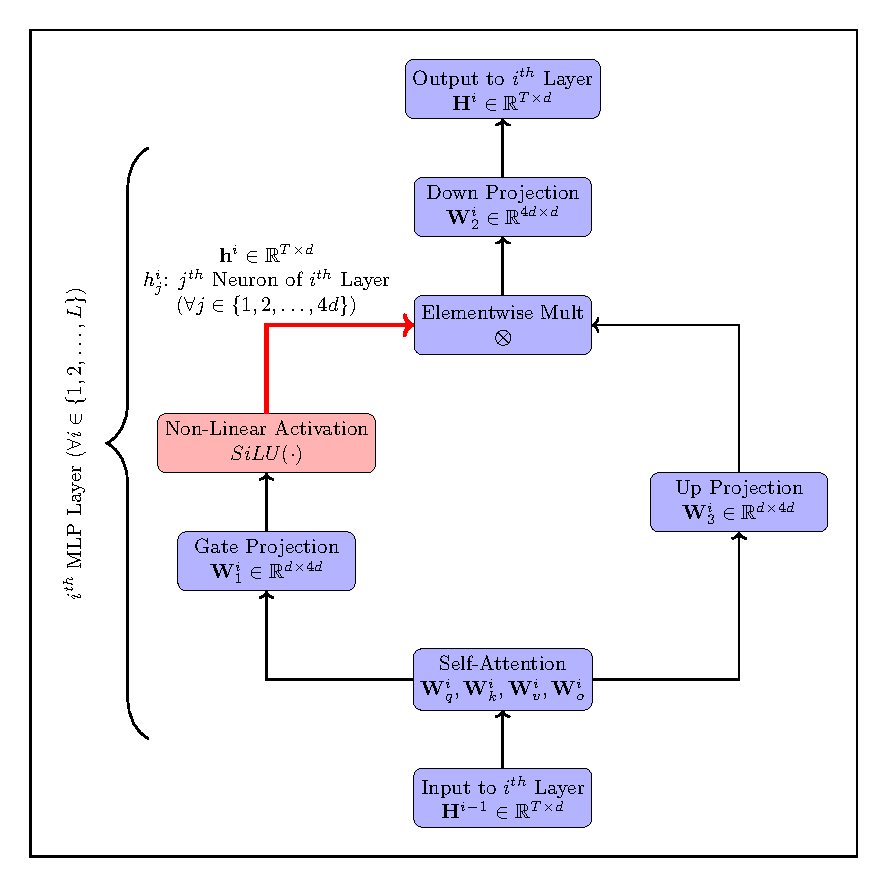
\includegraphics[width=\textwidth]{Chapters/Chapter_3/mlp.pdf} % Adjust the width as needed
	\caption{Architecture of MLP module in LLaMA model}
	\label{fig:mlp}
\end{figure}

\section{Dataset for Neuron Identification}

For the purpose of identifying language-specific neurons, we utilize a subset of the Wikipedia dataset spanning 15 languages:
\[
\text{\{en, fr, es, vi, id, ja, zh, bn, hi, ta, te, mr, ur, kn, ml, pa\}}.
\]
Each language's dataset is preprocessed and passed through pretrained large language models (LLMs). The activations are then collected from the MLP modules of the models.

\textbf{Dataset Description:}
The Wikipedia dataset [\cite{wikidump}] for each language contains a sequence of tokenized text data. Each tokenized sequence has a maximum length of $T_{\max} = 512$. For every sequence, we compute the activations from the MLP module, followed by averaging the activations at each neuron position across all sequences. This provides a language-specific profile for every neuron $(i, j)$ in the model.

\textbf{Activation Collection:} 
Given a pretrained LLM, let the MLP activation for the $i^\text{th}$ layer and the $j^\text{th}$ neuron in a specific language be represented by $h_{i,j}^t \in \mathbb{R}$, where $t$ indexes the token positions in a sequence of length $T$. The average activation of a neuron across all token positions for a given sequence is computed as:
\begin{equation}
\bar{h}_{i,j} = \frac{1}{T} \sum_{t=1}^{T} h_{i,j}^t,
\end{equation}
where $h_{i,j}^t$ is the neuron activation corresponding to the $t^\text{th}$ token.

\textbf{Language-Specific Activations:}
For each language $l$ in the dataset, we compute the average activation of each neuron $(i, j)$ over all sequences $S_l$ in the dataset:
\begin{equation}
h_{i,j}^l = \frac{1}{|S_l|} \sum_{s \in S_l} \bar{h}_{i,j}^{(s)},
\end{equation}
where $h_{i,j}^l$ represents the average activation of the $j^\text{th}$ neuron in the $i^\text{th}$ layer for language $l$, and $|S_l|$ denotes the number of sequences for language $l$.


\section{Statistics of Neuron Activation}

The statistics of neuron activation are precomputed to analyze language-specific patterns in the MLP layers of the pretrained large language models (LLMs). These statistics include mean, standard deviation, and quantiles (e.g., 5th, 10th, 25th, 50th, 75th, 90th, and 95th percentiles) of the neuron activations for each language in the dataset. The computations are performed across all layers and neurons within the MLP modules.

\textbf{Activation Mean and Standard Deviation:} The mean activation of a neuron $(i, j)$ in the $t^\text{th}$ token position is computed as:
\begin{equation}
\mu_{i,j} = \frac{1}{T} \sum_{t=1}^T h_{i,j}^t,
\end{equation}
where $h_{i,j}^t$ is the activation of the $(i,j)$ neuron for the $t^\text{th}$ token, and $T$ is the total number of tokens in a sequence. Similarly, the standard deviation of the activations is calculated as:
\begin{equation}
\sigma_{i,j} = \sqrt{\frac{1}{T} \sum_{t=1}^T (h_{i,j}^t - \mu_{i,j})^2}.
\end{equation}

\textbf{Quantiles of Activation:} Quantile-based statistics provide insights into the distribution of activations for each neuron. The $q$-quantile activation value, denoted as $P_q$, is defined as:
\begin{equation}
P_q(h_{i,j}) = \inf \left\{x \in \mathbb{R} : F_{h_{i,j}}(x) \geq q \right\},
\end{equation}
where $F_{h_{i,j}}(x)$ is the cumulative distribution function (CDF) of the activations for neuron $(i, j)$. Commonly computed quantiles include:
\[
P_{50}, \, P_{75}, \, P_{90}, \, P_{95}, \, P_{25}, \, P_{10}, \, P_{5}.
\]

\textbf{Language-Specific Aggregation:} For a given language $l$ and all sequences in the dataset, the mean and other statistics are aggregated across all token positions and batches. Let $S_l$ denote the set of sequences for language $l$, and $B$ represent the batch size. The aggregated mean activation for neuron $(i, j)$ is computed as:
\begin{equation}
\bar{\mu}_{i,j}^l = \frac{1}{|S_l|} \sum_{b=1}^B \sum_{s \in S_l} \mu_{i,j}^{(s,b)},
\end{equation}
where $\mu_{i,j}^{(s,b)}$ is the mean activation of neuron $(i, j)$ for the $s^\text{th}$ sequence in the $b^\text{th}$ batch.

\section {Methods for Neuron Identification}

\subsection{LAPE}

Language Activation Probability Entropy (LAPE) [\cite{tang2024languagespecific}] is a method designed to identify neurons that exhibit language-specific behavior across multiple languages. This metric quantifies the entropy of normalized activation probabilities for each neuron across the given set of languages.

\textbf{Step 1: Compute Activation Probabilities.} 
For a pretrained large language model with $L$ layers and $4d$ neurons per layer, the activation of a neuron $(i, j)$ in response to a sequence $X^l \in \mathbb{R}^{N \times T}$ (where $N$ is the number of sequences, and $T$ is the number of tokens per sequence) for a language $l$ is denoted as $h_{i,j}^l$. The unnormalized activation probability for neuron $(i, j)$ is given by:
\begin{equation}
	p_{i,j}^l = \mathbb{E}\left[\mathbb{I}\left(h_{i,j}^l > 0\right)\right],
\end{equation}
where $\mathbb{I}$ is the indicator function that returns $1$ if the activation $h_{i,j}^l$ is greater than zero, and $0$ otherwise. The expectation is computed over all tokens in all sequences for language $l$.

\textbf{Step 2: Normalize Activation Probabilities.} 
The normalized activation probability is computed across $k$ languages to ensure a valid probability distribution:
\begin{equation}
	P_{i,j}^l = \frac{p_{i,j}^l}{\sum_{l=1}^k p_{i,j}^l}, \quad \forall i \in \{1, \dots, L\}, \, \forall j \in \{1, \dots, 4d\}.
\end{equation}

\textbf{Step 3: Compute Language Activation Probability Entropy.} 
The entropy of the normalized activation probabilities for each neuron $(i, j)$ is computed as:
\begin{equation}
	\text{LAPE}(i, j) = - \sum_{l=1}^k P_{i,j}^l \log P_{i,j}^l, \quad \forall i \in \{1, \dots, L\}, \, \forall j \in \{1, \dots, 4d\}.
\end{equation}
This measures the uncertainty in the activation distribution of a neuron across the $k$ languages. Figure~\ref{fig:lape} shows the procedure of computing LAPE for a neuron.

\textbf{Step 4: Apply Threshold and Select Neurons.} 
To identify neurons with significant language-specific behavior, a threshold is defined based on the $95^\text{th}$ percentile of the unnormalized activation probabilities:
\begin{equation}
	\text{Threshold} = \text{Quantile}_{0.95}\left(p_{i,j}^l \, | \, \forall i, j, l\right).
\end{equation}
A neuron $(i, j)$ is considered for language-specific analysis only if:
\begin{equation}
	\exists l \in \{1, \dots, k\} \, \text{such that} \, p_{i,j}^l > \text{Threshold}.
\end{equation}

\textbf{Step 5: Select Top Neurons Based on LAPE.} 
Only 1\% neurons with the lowest LAPE values are selected for language-specific analysis, where $m$ is defined as:
\begin{equation}
	m = \frac{1 \times 4d \times L}{100}.
\end{equation}
The top \(m\) neurons are identified by sorting the LAPE values and selecting the indices of the \(m\) smallest values:
\begin{equation}
	\text{Top}_m(\text{Lang\_Set}) = \text{argsort\_ascending}_m \left\{\text{LAPE}(i,j) \,|\, \forall i, j, \exists l \,\, s.t. \,\,  p_{i,j}^l > \text{Threshold} \right\}.
\end{equation}
This ensures that only the most language-specific neurons are retained for further interpretation. 

\textbf{Step 6: Identify Language-Specific Neuron Sets.} 
For each neuron $(i, j)$ in the selected set, the language-specific set is defined as:
\begin{equation}
	\text{Lang\_Spec\_Set}(i, j) = \left\{ l \, | \, p_{i,j}^l > \text{Threshold}, (i,j) \in \text{Lang\_Set} \right\}.
\end{equation}

A neuron is considered specific to a subset of languages if:
\begin{equation}
	\text{Lang\_Spec\_Set}(i, j) \subseteq \{1, 2, \dots, k\}.
\end{equation}

\begin{figure}[ht]
	\centering
	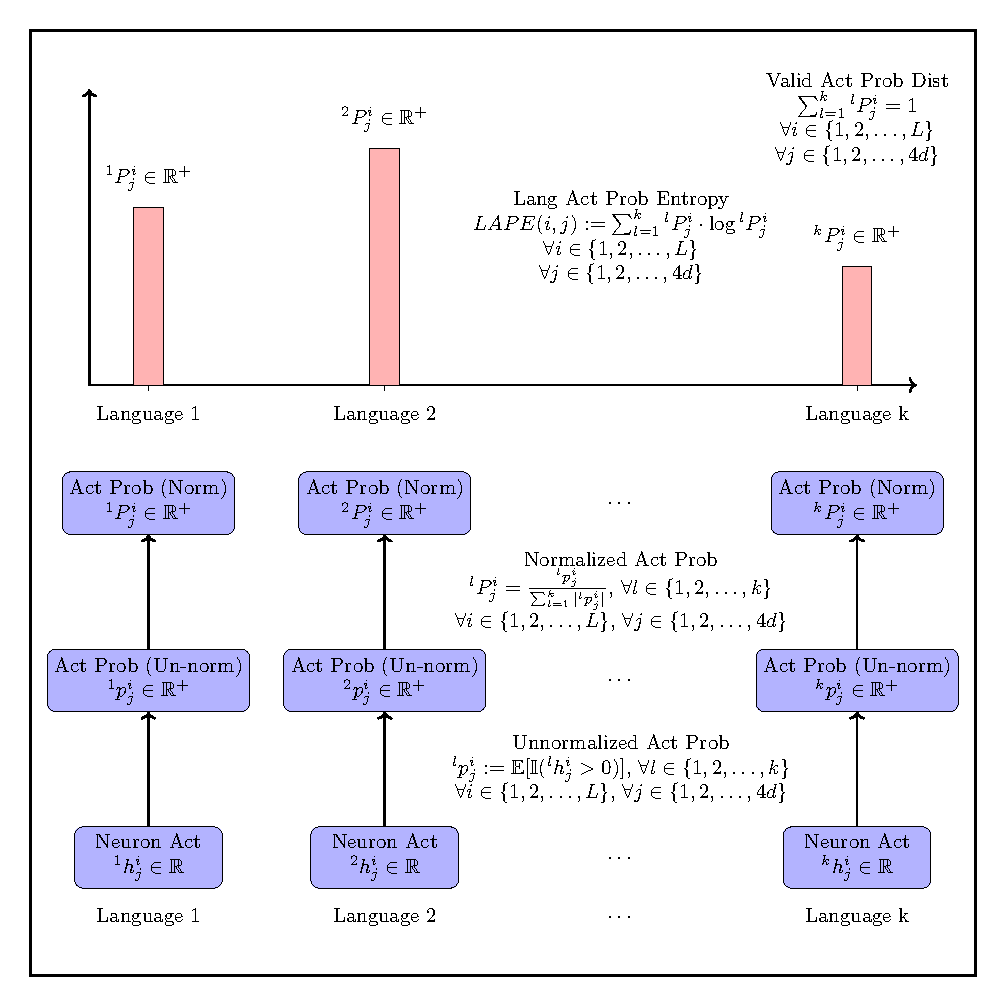
\includegraphics[width=\textwidth]{Chapters/Chapter_3/lape.pdf} % Adjust the width as needed
	\caption{Procedure of computing LAPE for a neuron.}
	\label{fig:lape}
\end{figure}

\subsection{Activation Based Methods}

\textbf{Absolute Activation:} The absolute activation metric measures the mean absolute activation of each neuron \((i, j)\) in the \(i^\text{th}\) layer across all tokens in a sequence for a language \(l\). This is computed as:
\begin{equation}
	r_{i,j}^l = \mathbb{E}\left[\left| h_{i,j}^l \right|\right],
\end{equation}
where \( h_{i,j}^l \) is the activation of neuron \((i, j)\) for language \(l\), and the expectation is taken over all tokens and sequences. This metric identifies neurons with consistently high absolute activations, which are indicative of their overall importance in representing language features.

\textbf{Activation Probability Zero:} The activation probability zero metric measures the fraction of times a neuron \((i, j)\) has a positive activation for a language \(l\). It is defined as:
\begin{equation}
	r_{i,j}^l = \mathbb{E}\left[\mathbb{I}\left(h_{i,j}^l > 0\right)\right],
\end{equation}
where \(\mathbb{I}\) is the indicator function that returns 1 if \(h_{i,j}^l > 0\), and 0 otherwise. This metric captures the frequency of a neuron's activation, providing insights into its contribution to language-specific representations.

\textbf{Activation Probability Mean:} The activation probability mean measures the probability of a neuron's activation exceeding the mean activation value for its layer, \(\mu_{i,j}^l\), for a language \(l\). It is computed as:
\begin{equation}
	r_{i,j}^l = \mathbb{E}\left[\mathbb{I}\left(h_{i,j}^l > \mu_{i,j}^l\right)\right],
\end{equation}
where \(\mu_{i,j}^l\) represents the average activation of neuron \((i, j)\) in the \(i^\text{th}\) layer for language \(l\). This metric identifies neurons with activations that are consistently above the average, highlighting neurons that are highly responsive to language-specific features.

\textbf{Activation Probability 90p:} The activation probability 90p measures the probability of a neuron's activation exceeding the 90th percentile activation value for its layer, \(\text{P90}_{i,j}^l\), for a language \(l\). This is given by:
\begin{equation}
	r_{i,j}^l = \mathbb{E}\left[\mathbb{I}\left(h_{i,j}^l > \text{P90}_{i,j}^l\right)\right],
\end{equation}
where \(\text{P90}_{i,j}^l\) represents the 90th percentile of the activations of neuron \((i, j)\) in the \(i^\text{th}\) layer for language \(l\). This metric identifies neurons that exhibit rare but significant activations, which may correspond to specialized processing for certain linguistic features.

Language-specific neurons are identified based on activation values computed across different languages. For each language, activations are collected, and neurons that exhibit the highest relevance are selected using the following process.

\textbf{Step 1: Compute Activation Relevance.} 
For each language \(l \in \{1, 2, \dots, k\}\), compute the activation relevance values for all neurons \((i, j)\) in the pretrained model. Let the relevance for neuron \((i, j)\) in the \(i^\text{th}\) layer for language \(l\) be denoted as \(r_{i,j}^l\). This relevance is calculated using one of the activation probability methods, such as:
\begin{equation}
	r_{i,j}^l = \mathbb{E}\left[\mathbb{I}\left(h_{i,j}^l > 0\right)\right],
\end{equation}
or other methods such as absolute activation or percentile-based thresholds, depending on the desired analysis.

\textbf{Step 2: Aggregate Relevance Across Layers and Neurons.} 
For each language \(l\), the computed relevance values \(r_{i,j}^l\) are aggregated across all layers and neurons. The total number of layers is denoted by \(L\), and the dimensionality of the neurons in each layer is \(4d\). The relevance tensor for language \(l\) is represented as:
\begin{equation}
	R^l = \{r_{i,j}^l \, | \, i \in \{1, \dots, L\}, \, j \in \{1, \dots, 4d\}\}.
\end{equation}

\textbf{Step 3: Select Top Neurons.} 
For each language \(l\), the top \(m\) neurons with the highest relevance values are selected. The value of \(m\) is determined as a small fraction of the total number of neurons in the model:
\begin{equation}
	m = \frac{0.125 \times L \times 4d}{100}.
\end{equation}
The top \(m\) neurons are identified by sorting the relevance values in \(R^l\) and selecting the indices of the \(m\) largest values:
\begin{equation}
	\text{Top}_m(R^l) = \text{argsort\_descending}_m \left\{r_{i,j}^l | \forall i, j\right\}.
\end{equation}

\textbf{Step 4: Map Neurons to Layers and Positions.} 
The indices of the top \(m\) neurons are mapped back to their corresponding layers and positions. For each language \(l\), the selected neurons are represented as:
\begin{equation}
	N^l = \{(i, j) \, | \, (i, j) \in \text{Top}_m(R^l)\},
\end{equation}
where \(N^l\) is the set of top \(m\) neurons for language \(l\).

This process ensures that neurons with the highest language-specific relevance are identified for each language. These neurons can then be analyzed further to understand their behavior and contribution to language modeling tasks.

\subsection{Task Neurons for a Language}

In this method, we introduce an alternative method based on task-specific neurons computed from the task specific dataset (for example XNLI dataset). Unlike language-specific neurons, which are computed using activation patterns derived from Wikipedia sentences, the task neurons are computed by processing the training sentences from the task dataset for each respective language. This modification allows the identification of neurons that are not only language-specific but also task-specific, capturing finer granularity of representations relevant to the classification task.

\textbf{Activation of Task-Specific Neurons:} The activation pattern for task-specific neurons is derived as:
\begin{equation}
	h^{\text{task}}_{ij} = \text{stat}_{ij}^{\text{task}}, \quad \forall \text{stat} \in \{\mu, p_{90}, p_{75}, p_{50}, p_{25}, p_{10}, p_{5}\},
\end{equation}
where:
\begin{itemize}
	\item $h^{\text{task}}_{ij}$ represents the activation for the $i$-th layer and $j$-th neuron under task-specific conditions.
	\item $\text{stat}_{ij}^{\text{task}}$ denotes the statistical activation computed over all task specific training sentences in a given language.
	\item The set $\{\mu, p_{90}, p_{75}, p_{50}, p_{25}, p_{10}, p_{5}\}$ represents the mean, 90th percentile, 75th percentile, and other quantile thresholds used to analyze neuron activation levels.
\end{itemize}

Once the activation is computed for a task, then we can apply the LAPE or any activation based methods to compute the task specific neurons.

\section{Neuron Fine-Tuning using LoRA for a Task}

\textbf{LoRA (Low-Rank Adaptation)}: LoRA [\cite{lora}] introduces a mechanism to fine-tune a subset of parameters in neural networks, focusing on reducing computational overhead. For our application, we utilize LoRA to specifically fine-tune targeted neurons in the MLP layer while freezing others. This method ensures that the pretrained parameters \(W_{pt}\) remain untouched, and \(\Delta W\) represents the modifications applied to the network during fine-tuning.

\textbf{Fine-Tuning with LoRA AB Decomposition.} The matrix \(\Delta W\) is expressed as:
\begin{equation}
	\Delta W = A \cdot B,
\end{equation}
where \(A \in \mathbb{R}^{d_{in} \times r}\) and \(B \in \mathbb{R}^{r \times d_{out}}\) are low-rank matrices. The rank \(r\) is typically much smaller than \(d_{in}\) or \(d_{out}\), reducing the number of trainable parameters. Masks are applied to \(A\) and \(B\) to control the fine-tuning of specific neurons:
\begin{equation}
	A = \text{masked\_A} \cdot A_t, \quad B = \text{masked\_B} \cdot B_t,
\end{equation}
where \(\text{masked\_A}\) and \(\text{masked\_B}\) are binary masks, and \(A_t\) and \(B_t\) are trainable parameters.

\textbf{Description of Masked Matrices:}

The binary masks \(\text{masked\_A}\) and \(\text{masked\_B}\) are defined to control the fine-tuning process by selectively freezing specific neurons.
\[
	\text{masked\_A} \in \mathbb{R}^{d_{in} \times r}, \quad
	\text{masked\_B} \in \mathbb{R}^{r \times d_{out}},
\]
where \(d_{in}\) and \(d_{out}\) are the input and output dimensions of the layer, and \(r\) is the rank of the LoRA decomposition.

\textbf{Masked Matrix \(\text{masked\_A}\):}
\(\text{masked\_A}\) is defined as:
\begin{equation}
	[\text{masked\_A}]_{ij} = 1, \quad \forall i \in \{1, \dots, d_{in}\}, \, \forall j \in \{1, \dots, r\}.
\end{equation}
This indicates that no masking is applied to the rows of \(A\), and all elements of \(\text{masked\_A}\) are set to 1.

\textbf{Masked Matrix \(\text{masked\_B}\):}
For \(\text{masked\_B}\), specific columns corresponding to frozen neurons are set to 0. For a neuron index \(j_f \in \text{Frozen Neurons}\), the mask is defined as:
\begin{equation}
	[\text{masked\_B}]_{ij} = 
	\begin{cases} 
		0, & \text{if } j = j_f, \, j_f \in \text{Frozen Neurons}, \\
		1, & \text{otherwise}.
	\end{cases}
\end{equation}

\textbf{Final Masking Condition:}
The effective masked matrices for \(A\) and \(B\) are:
\begin{equation}
	A = \text{masked\_A} \cdot A_t, \quad
	B = \text{masked\_B} \cdot B_t,
\end{equation}
where \(A_t \in \mathbb{R}^{d_{in} \times r}\) and \(B_t \in \mathbb{R}^{r \times d_{out}}\) are the trainable LoRA matrices.

This masking ensures that updates to the frozen neurons are completely suppressed, while other neurons remain trainable during fine-tuning.

\textbf{Frozen Neurons.} To freeze specific neurons, columns of \(B\) corresponding to the frozen neurons are masked with zeros. For neuron indices \(j\) in the set of frozen neurons, we ensure:
\begin{equation}
	\Delta W_{i,j} = 0, \quad \forall i.
\end{equation}
This prevents any updates to these neurons during fine-tuning.

\textbf{Final Output.} The fine-tuned output of the MLP layer is given by:
\begin{equation}
	y = x \cdot W + x \cdot \Delta W,
\end{equation}
where \(W\) is the original weight matrix, and \(\Delta W\) introduces targeted updates through LoRA.

\textbf{Targeted Language Neurons.} Language-specific neurons are identified and fine-tuned using LoRA. This targeted approach ensures that only the relevant neurons for a particular language are adapted while the others remain unchanged. For the frozen neurons, \(\Delta W\) remains zero:
\begin{equation}
	\Delta W_{i,j} = 0, \quad \text{if } j \in \text{Frozen Neurons}.
\end{equation}

\textbf{Additional Fine-Tuning.} Besides fine-tuning the MLP layer, the attention mechanisms (\(q, k, v, o\) projections) and the task-specific classifier head are always fine-tuned using LoRA. This ensures the overall task-specific performance is preserved while leveraging the language neurons for targeted adaptation. Figure~\ref{fig:lora} shows the procedure of finetuning target neurons using LoRA.

\begin{figure}[ht]
	\centering
	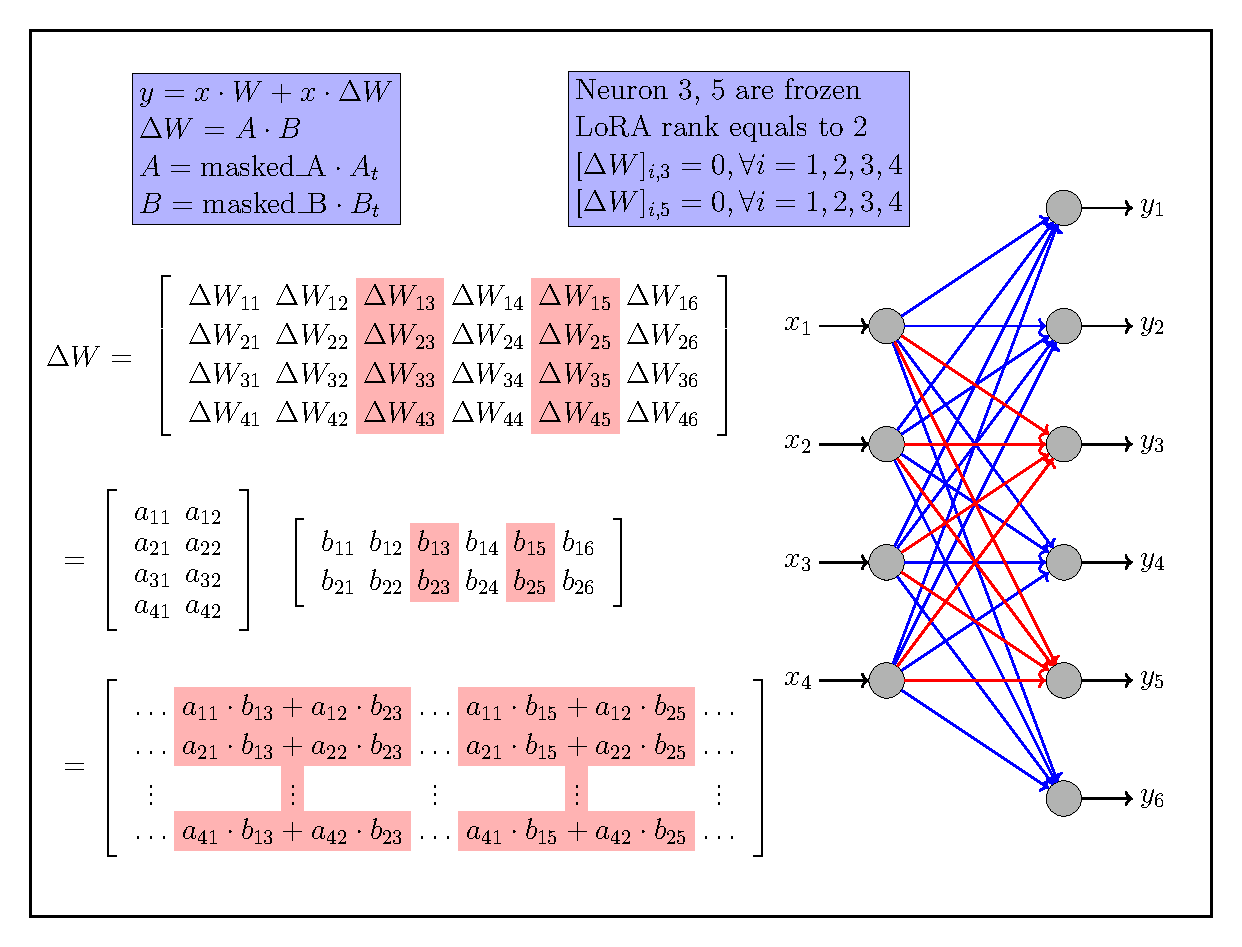
\includegraphics[width=\textwidth]{Chapters/Chapter_3/lora.pdf} % Adjust the width as needed
	\caption{LoRA fine tuning method for target neurons.}
	\label{fig:lora}
\end{figure}







% Chapter Template

\chapter{Experiments}\singlespacing % Main chapter title

\label{Chapter4} % Change X to a consecutive number; for referencing this chapter elsewhere, use \ref{ChapterX}

\lhead{Chapter 4. \emph{Experiments}} % Change X to a consecutive number; this is for the header on each page - perhaps a shortened title

%----------------------------------------------------------------------------------------
%	SECTION 1
%----------------------------------------------------------------------------------------

\section{Task and Dataset: XNLI}

\textbf{The Cross-lingual Natural Language Inference (XNLI) task} is a benchmark designed to evaluate the capability of large language models (LLMs) to perform reasoning across multiple languages. The goal is to classify the relationship between a premise and a hypothesis into one of three categories: \textit{entailment}, \textit{neutral}, or \textit{contradiction}. This task tests the ability of the model to generalize semantic relationships beyond the English language, making it a challenging benchmark for multilingual models.

\textbf{Dataset Overview:} The XNLI dataset contains annotated sentence pairs across 15 languages. In our experiments, we focus on English (\textit{en}) as the source language and Vietnamese (\textit{vi}), Hindi (\textit{hi}) and Urdu (\textit{ur}) as target languages. The dataset for each language can be represented as:
\begin{equation}
	\mathcal{D}_l = \{(x_p^i, x_h^i, y^i) \,|\, x_p^i, x_h^i \in \mathcal{X}_l, \, y^i \in \{0, 1, 2\}\},
\end{equation}
where \(x_p^i\) and \(x_h^i\) denote the premise and hypothesis sentences in language \(l\), and \(y^i\) is the corresponding label indicating the relationship.

\textbf{Tokenization and Preprocessing:} Each sentence pair \((x_p^i, x_h^i)\) is concatenated with a special token to form the input:
\begin{equation}
	x^i = x_p^i + \text{[EOS]} + x_h^i,
\end{equation}
where \([EOS]\) represents the end-of-sequence token. The concatenated input is tokenized into a sequence of tokens \(\{t_1, t_2, \dots, t_T\}\) with a maximum sequence length \(T = 512\).

\textbf{Train and Test Splits:} The dataset is divided into training and testing subsets for each language:
\begin{equation}
	\mathcal{D}_l = \mathcal{D}_l^\text{train} \cup \mathcal{D}_l^\text{test}, \quad \mathcal{D}_l^\text{train} \cap \mathcal{D}_l^\text{test} = \emptyset.
\end{equation}
For the experiments, a fraction \(\mathcal{F} \subset \mathcal{D}_l^\text{train}\) is used to train the model. The size of \(\mathcal{F}\) is determined as:
\begin{equation}
	|\mathcal{F}| = \text{frac} \times |\mathcal{D}_l^\text{train}|,
\end{equation}
where \(\text{frac}\) is the fraction of the training dataset used.

\textbf{Multilingual Challenges:} In the XNLI task, transferring knowledge from English to other languages like Vietnamese and Hindi requires the model to overcome both semantic and structural differences in language. This transfer is tested by evaluating the zero-shot performance on the target languages without directly training on their data. The objective of this task is to fine-tune LLaMA3, a large language model, on the XNLI dataset to improve cross-lingual inference capabilities. The experiments are designed to test the effectiveness of various fine-tuning setups and analyze the role of language-specific neurons in improving performance across multiple languages.

\section{Baseline Experiments}

The baseline experiments establish a foundation for evaluating the performance of different fine-tuning setups on the XNLI task. We include two baselines: zero-shot evaluation of a model fine-tuned on English (\textit{en}) XNLI data and direct fine-tuning on the target language (\textit{vi}) XNLI data. These baselines provide a comparative framework to assess the impact of fine-tuning specific language neurons using LoRA.

\textbf{Zero-Shot Baseline:} The first baseline involves fine-tuning the pretrained model on the English XNLI dataset. Let \(\mathcal{M}_\text{en}\) denote the model fine-tuned on English data. The zero-shot evaluation involves testing \(\mathcal{M}_\text{en}\) on Vietnamese XNLI datasets without further training. The evaluation metric, accuracy, is defined as:
\begin{equation}
	\text{Accuracy} = \frac{\sum_{i=1}^N \mathbb{I}(\hat{y}^i = y^i)}{N},
\end{equation}
where \(N\) is the total number of test examples, \(y^i\) is the ground truth label, \(\hat{y}^i\) is the predicted label, and \(\mathbb{I}(\cdot)\) is the indicator function.

\textbf{Direct Fine-Tuning Baseline:} The second baseline involves directly fine-tuning the pretrained model on the Vietnamese XNLI dataset. Let \(\mathcal{M}_\text{vi}\) denote the model fine-tuned on Vietnamese data. This baseline establishes an upper bound for performance on the Vietnamese XNLI task, as the model is explicitly trained on the target language data. We again use the accuracy as evaluation metric.

\section{Experiment Goals}

The primary objective of this work is to improve the zero-shot performance of the model on the target language, such as Vietnamese (\textit{vi}), without utilizing any target language training data. This constraint is critical to ensure that the model remains agnostic to the specific characteristics of the target language during training, thereby simulating a real-world cross-lingual transfer learning scenario.

\textbf{Baseline Comparison:} In this setup, we consider two baselines:
\begin{itemize}
	\item \textbf{Baseline 1: Zero-Shot Performance on \textit{vi} using English Training Data.} This baseline involves fine-tuning the pretrained model on the English (\textit{en}) XNLI dataset (\(\mathcal{M}_\text{en}\)) and evaluating its zero-shot performance on the Vietnamese (\textit{vi}) test set. This represents the starting point of cross-lingual transfer without any modifications to the model architecture or targeted interventions.
	\item \textbf{Baseline 2: Performance on \textit{vi} using Direct Fine-Tuning on \textit{vi} Data.} This baseline involves directly fine-tuning the pretrained model on the Vietnamese (\textit{vi}) XNLI dataset (\(\mathcal{M}_\text{vi}\)). It provides an upper bound on performance since it leverages target language training data.
\end{itemize}

\textbf{Objective Constraints:} While the ultimate goal is to improve the zero-shot performance on the \textit{vi} test set, it is imperative to operate under the following constraints:
\begin{enumerate}
	\item No target language (\textit{vi}) training data can be used during the fine-tuning process.
	\item Only the English (\textit{en}) XNLI training data is available for model training and intervention.
	\item The interventions must be limited to model surgery techniques, such as fine-tuning specific neurons or modifying activation patterns.
\end{enumerate}

\textbf{Target Metric:} The improvement in zero-shot performance is quantified as:
\begin{equation}
	\Delta_\text{ZS} = \text{Accuracy}(\mathcal{M}_\text{experiment}) - \text{Accuracy}(\mathcal{M}_\text{en}),
\end{equation}
where \(\mathcal{M}_\text{experiment}\) refers to the model modified through various intervention strategies, and \(\mathcal{M}_\text{en}\) refers to the baseline model fine-tuned on \textit{en}.

\textbf{Goal:} The overarching goal is to maximize \(\Delta_\text{ZS}\), thereby surpassing the performance of Baseline 1 (\(\mathcal{M}_\text{en}\)) through innovative techniques such as:
\begin{itemize}
	\item Fine-tuning language-specific neurons identified for the target language (\textit{vi}) using only the \textit{en} training data.
	\item Utilizing statistical activation patterns (\textit{e.g., mean, quantile-based thresholds}) to intervene in neuron activations during inference.
	\item Applying LoRA (Low-Rank Adaptation) to selectively fine-tune specific components such as \textit{qkv} projections and classification heads while freezing other parts of the model.
\end{itemize}

\textbf{Limitations:} By design, the performance of any intervention cannot exceed Baseline 2 (\(\mathcal{M}_\text{vi}\)), as that baseline uses direct training data from the target language. However, our approach aims to close the gap between Baseline 1 (\(\mathcal{M}_\text{en}\)) and Baseline 2 (\(\mathcal{M}_\text{vi}\)) as much as possible through zero-shot strategies.

\section{Targeted Neuron Fine-tuning Experiment}

This section outlines the experimental setups designed to improve the zero-shot performance of the model on the Vietnamese (\textit{vi}) XNLI dataset. Four configurations are explored, each using different strategies to fine-tune the model, while adhering to the constraint of using only English (\textit{en}) training data during fine-tuning. The experiments aim to utilize targeted interventions to improve performance by selectively tuning neurons and applying LoRA-based adaptations.

\textbf{Setup A: Standard Fine-Tuning with LoRA.} In this setup, the pretrained model is fine-tuned on the English (\textit{en}) XNLI dataset using LoRA. The fine-tuning is applied to the query (\(q\)), key (\(k\)), value (\(v\)), and output (\(o\)) projection matrices (\(W_q^i\), \(W_k^i\), \(W_v^i\), \(W_o^i\)) and the classification head. The resulting model is evaluated on the Vietnamese (\textit{vi}) dataset in a zero-shot setting. Additionally, the \textit{vi}-specific activations are substituted by statistical activation patterns such as mean (\(\mu\)), 90\textsuperscript{th} percentile, and others, defined as:
\begin{equation}
	\hat{h}_{j}^{i,\text{vi}} = \text{stat}_{j}^{i,\text{vi}}, \quad \forall \, \text{stat} \in \{\text{mean}, 90p, 95p, 75p, 5p, 10p, 25p, 0\},
\end{equation}
where \(\hat{h}_{j}^{i,\text{vi}}\) represents the substituted activation for vi language for neuron \((i,j)\) in the MLP block.

\textbf{Setup B: Fine-Tuning with LoRA and English Neurons.} This setup builds on Setup A by incorporating fine-tuning of English-specific neurons identified in the MLP block. Let \(\mathcal{N}_\text{en}\) denote the set of English-specific neurons. During fine-tuning, the LoRA modifications (\(\Delta W\)) are applied to both the query-key-value-output projections and the English neurons, ensuring that:
\begin{equation}
	\Delta W_{j}^{i} = 0, \quad \forall j \notin \mathcal{N}_\text{en}.
\end{equation}
This targeted approach allows the model to specialize in English while preserving the generalization capacity of other neurons.

\textbf{Setup C: Fine-Tuning with LoRA and Target Language Neurons.} In this configuration, the focus shifts to fine-tuning target language such as Vietnamese-specific neurons (\(\mathcal{N}_\text{vi}\)). During fine-tuning, the LoRA modifications (\(\Delta W\)) are applied to both the query-key-value-output projections and the Vietnamese neurons, ensuring that:
\begin{equation}
	\Delta W_{j}^{i} = 0, \quad \forall j \notin \mathcal{N}_\text{vi}.
\end{equation}
This ensures that only the Vietnamese-specific neurons are fine-tuned while others remain untouched.

\textbf{Setup D: Fine-Tuning with LoRA and Both English \& Target Language Neurons.} This setup combines the interventions from Setup B and Setup C, targeting both English and Vietnamese neurons. Let \(\mathcal{N}_\text{en,vi} = \mathcal{N}_\text{en} \cup \mathcal{N}_\text{vi}\) represent the union of English and Vietnamese neurons. During fine-tuning, the LoRA modifications (\(\Delta W\)) are applied to both the query-key-value-output projections and both the English \& Vietnamese neurons, ensuring that:
\begin{equation}
	\Delta W_{j}^{i} = 0, \quad \forall j \notin \mathcal{N}_\text{en,vi}.
\end{equation}
This strategy allows the model to simultaneously adapt to English and Vietnamese language-specific representations.

\textbf{Comparative Analysis:} After fine-tuning, the zero-shot performance on Vietnamese (\textit{vi}) XNLI data is measured using the accuracy metric. The performance improvements achieved through the setups are quantified by:
\begin{equation}
	\Delta_\text{ZS} = \text{Accuracy}(\mathcal{M}_\text{setup}) - \text{Accuracy}(\mathcal{M}_\text{en}),
\end{equation}
where \(\mathcal{M}_\text{setup}\) refers to the model fine-tuned using one of the experimental setups. These improvements are compared against the baselines to evaluate the efficacy of the targeted neuron fine-tuning strategies.







%%%%%%%%%%%%%%%%% Changes%%%%%%%%%%%%%%%%%%%%%%%%














































 
% Chapter Template

\chapter{Analysis and Results}\singlespacing % Main chapter title

\label{Chapter5} % Change X to a consecutive number; for referencing this chapter elsewhere, use \ref{ChapterX}

\lhead{Chapter 5. \emph{Analysis and Results}} % Change X to a consecutive number; this is for the header on each page - perhaps a shortened title

%----------------------------------------------------------------------------------------
%	SECTION 1
%----------------------------------------------------------------------------------------

\section{LAPE Experiments}

\subsection{Language Sets}

In this section, we define the different language sets used for evaluating the Language Activation Probability Entropy (LAPE) in the context of our experiments. The language sets are constructed to capture varying linguistic and typological characteristics across a diverse group of languages. The experimental results on these sets aim to analyze the impact of multilinguality on language-specific neuron activations.

\textbf{Set 1: Core Languages.} This set includes the core languages commonly supported by pretrained language models: 
\[
\text{Set 1} = \{\text{en}, \text{fr}, \text{es}, \text{vi}, \text{id}, \text{ja}, \text{zh}\}.
\]
These languages span across major linguistic families and represent both high-resource and typologically distinct languages.

\textbf{Set 2: Extended Core with Indian Languages.} To incorporate a mix of Western and Indian languages, this set is defined as:
\[
\text{Set 2} = \{\text{en}, \text{fr}, \text{vi}, \text{zh}, \text{bn}, \text{hi}, \text{te}, \text{mr}\}.
\]
Here, \(\text{bn}\) (Bengali), \(\text{hi}\) (Hindi), \(\text{te}\) (Telugu), and \(\text{mr}\) (Marathi) represent Indian languages, providing an interesting contrast to the Western languages in the set.

\textbf{Set 3: Indian Subset.} This set focuses exclusively on Indian languages:
\[
\text{Set 3} = \{\text{bn}, \text{hi}, \text{ta}, \text{te}, \text{mr}, \text{ur}, \text{kn}, \text{ml}, \text{pa}\},
\]
where \(\text{ta}\) (Tamil), \(\text{ur}\) (Urdu), \(\text{kn}\) (Kannada), \(\text{ml}\) (Malayalam), and \(\text{pa}\) (Punjabi) are included to cover a broader typological spectrum of Indian languages.

\textbf{Set 4: Core and Extended Languages.} Combining the core and extended sets, this set is defined as:
\[
\text{Set 4} = \{\text{en}, \text{fr}, \text{es}, \text{vi}, \text{id}, \text{ja}, \text{zh}, \text{bn}, \text{hi}, \text{te}\}.
\]
This allows for the comparison of results across a comprehensive multilingual setup.

\textbf{Set 5: All Languages.} This set includes all the languages in the experimental framework:
\[
\text{Set 5} = \{\text{en}, \text{fr}, \text{es}, \text{vi}, \text{id}, \text{ja}, \text{zh}, \text{bn}, \text{hi}, \text{ta}, \text{te}, \text{mr}, \text{ur}, \text{kn}, \text{ml}, \text{pa}\}.
\]

\textbf{Set 6: Indian Language Dominant.} This set focuses on Indian languages while retaining a few globally dominant ones:
\[
\text{Set 6} = \{\text{en}, \text{bn}, \text{hi}, \text{ta}, \text{te}, \text{mr}, \text{ur}, \text{kn}, \text{ml}, \text{pa}\}.
\]

The diversity of the language sets ensures a thorough evaluation of language-specific neuron behavior. By analyzing LAPE across these sets, we aim to uncover insights into the multilingual capabilities of the pretrained model and the role of specific languages in driving neuron activations.

\subsection{Language Neuron Distribution}

The Language Activation Probability Entropy (LAPE) method enables the identification of language-specific neurons in large language models. This section analyzes the distribution of language-specific neurons across different languages, their overlap, and their distribution across model layers for the selected sets of languages, namely \textbf{Set1} and \textbf{Set3}. These analyses are crucial for understanding how linguistic diversity is represented within the model and for designing strategies for targeted interventions.

\textbf{Language-Specific Neuron Counts:} The number of language-specific neurons for each language in \textbf{Set1} and \textbf{Set3} is illustrated in Figure \ref{fig:lang_neuron_distribution}. The LAPE method assigns neurons to languages based on their activation probabilities. Formally, the number of neurons for a language $l$ is computed as:
\begin{equation}
	N_l = \sum_{i=1}^{L} \sum_{j=1}^{4d} \mathbb{I}\left(p_{i,j}^l > \text{Threshold} \right) \cdot \delta\left( (i,j) \in \text{Lang\_Set} \right),
\end{equation}
where $N_l$ is the total number of neurons assigned to language $l$, $p_{i,j}^l$ denotes the un-normalized activation probability for a language neuron $(i,j) \in \text{Lang\_Set}$ and language $l$, and $\mathbb{I}$ is the indicator function. The threshold ensures that only the most prominent neurons are included.

\begin{figure}[ht]
	\centering
	\begin{tabular}{cc}
		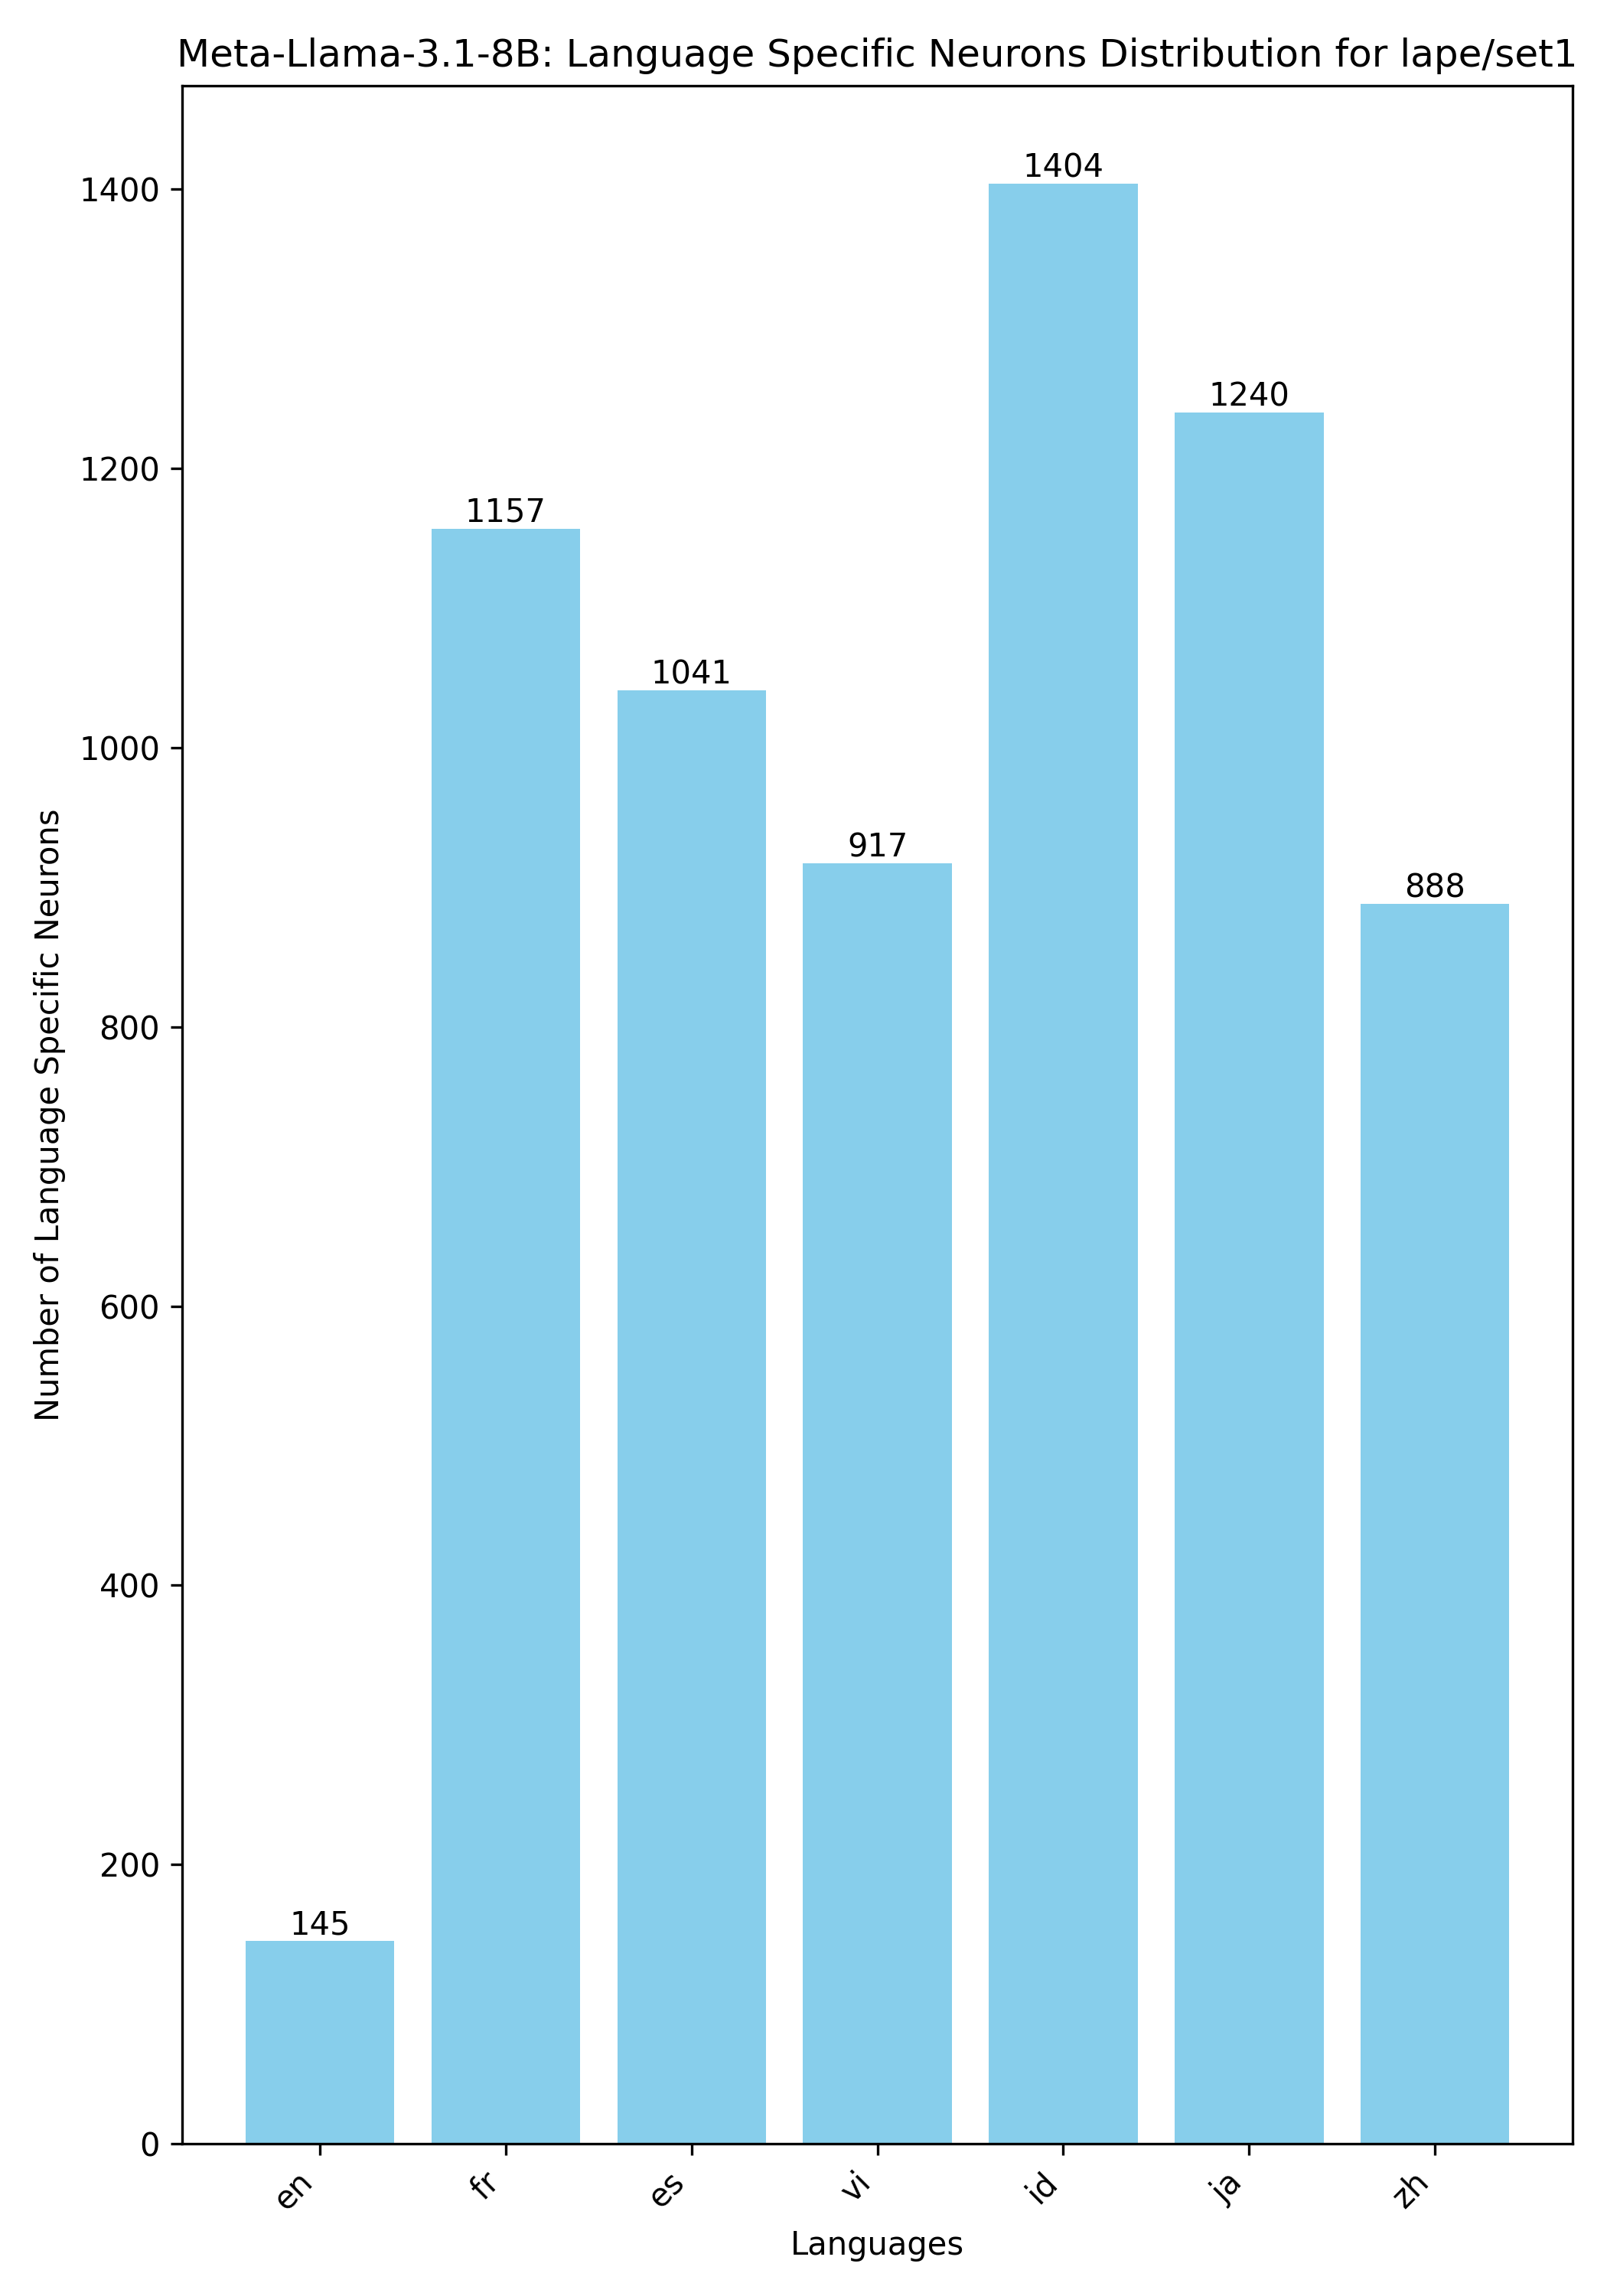
\includegraphics[width=0.45\textwidth]{Chapters/Chapter_5/lang_neurons/Meta-Llama-3.1-8B/lape/set1/lang_neuron_dist.png} &
		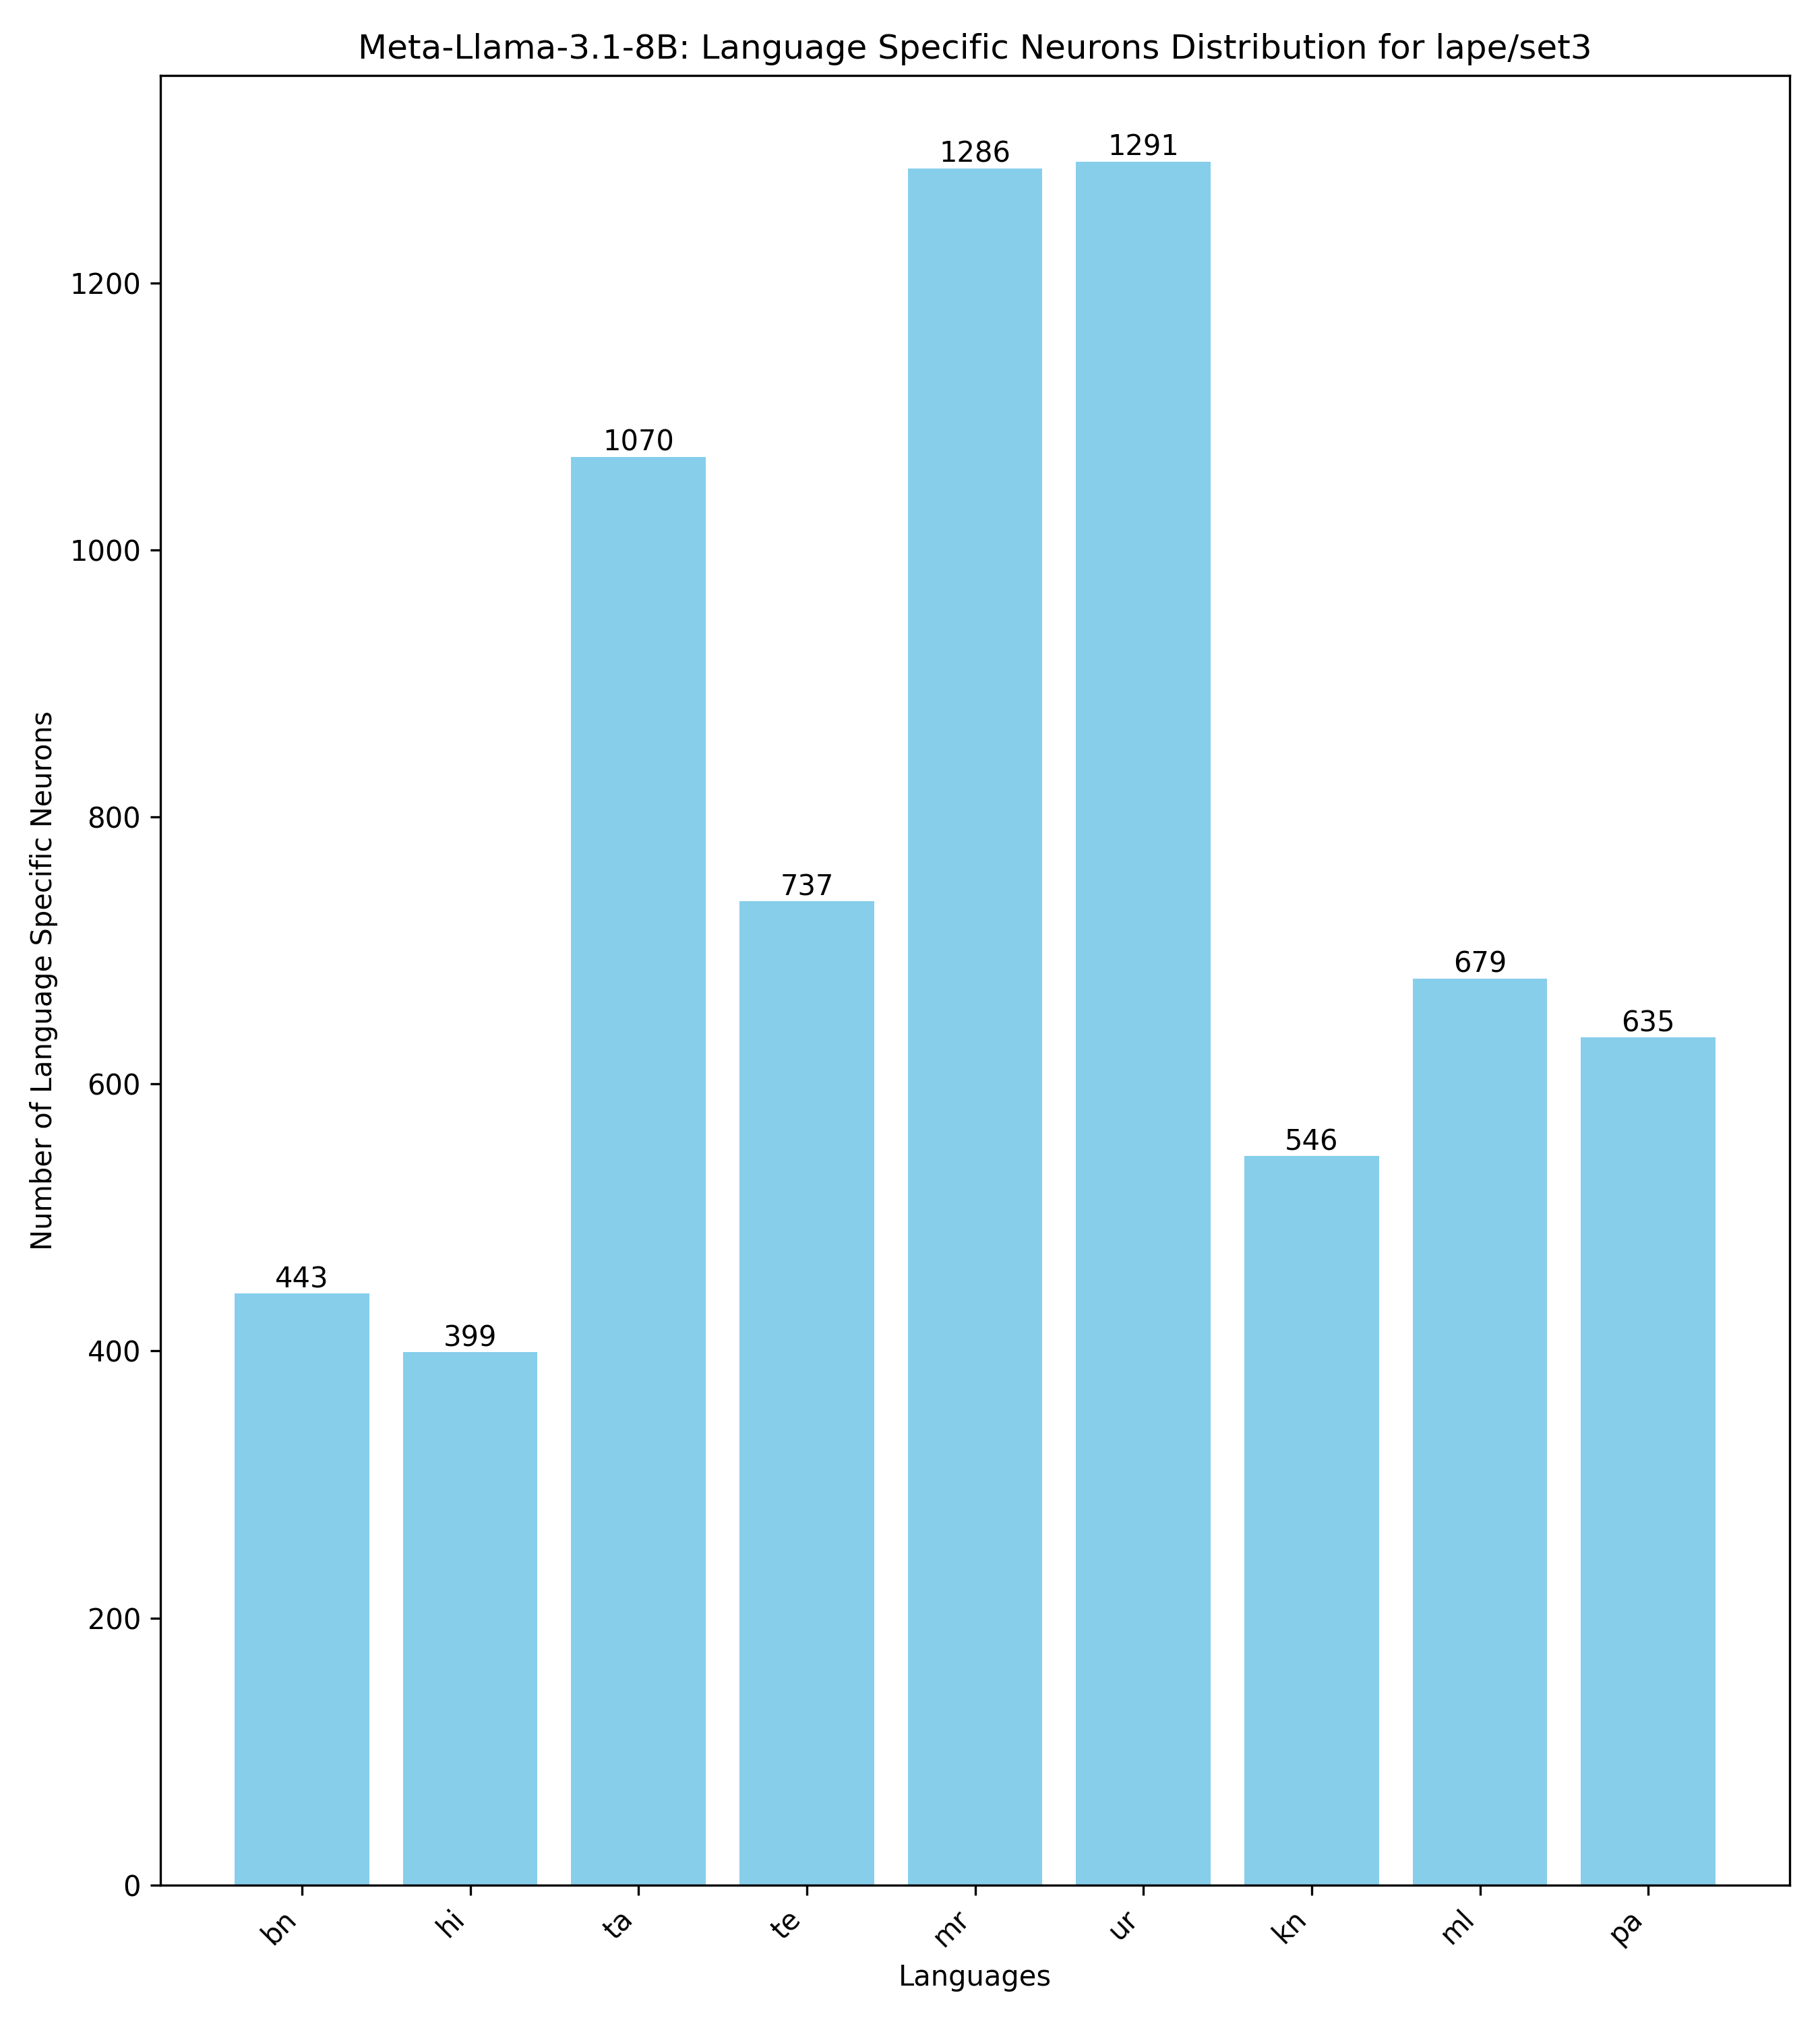
\includegraphics[width=0.45\textwidth]{Chapters/Chapter_5/lang_neurons/Meta-Llama-3.1-8B/lape/set3/lang_neuron_dist.png} \\
		\textbf{Set1: Language Neuron Distribution} &
		\textbf{Set3: Language Neuron Distribution}
	\end{tabular}
	\caption{Language-specific neuron distributions for LAPE method for Set1 and Set3.}
	\label{fig:lang_neuron_distribution}
\end{figure}

From Figure \ref{fig:lang_neuron_distribution}, it is evident that certain languages, such as \textit{id}, \textit{ja}, \textit{ur}, and \textit{mr}, have higher neuron counts, suggesting that the model dedicates more capacity to languages with rich morphology or syntactic structures. Conversely, \textit{en} consistently has the fewest neurons, likely due to its large amount of training data.

\textbf{Neuron Overlap Between Languages:} Figure \ref{fig:lang_neuron_overlap} illustrates the overlap of language-specific neurons between languages in Set1 and Set3. The overlap is formally calculated as:
\begin{equation}
	O_{l_1, l_2} = \sum_{i=1}^{L} \sum_{j=1}^{4d} \mathbb{I}\left(p_{i,j}^{l_1} > \text{Threshold}\right) \cdot \mathbb{I}\left(p_{i,j}^{l_2} > \text{Threshold}\right) \cdot \delta\left( (i,j) \in \text{Lang\_Set} \right),
\end{equation}
where $O_{l_1, l_2}$ represents the number of neurons shared between languages $l_1$ and $l_2$. 

\begin{figure}[ht]
	\centering
	\begin{tabular}{cc}
		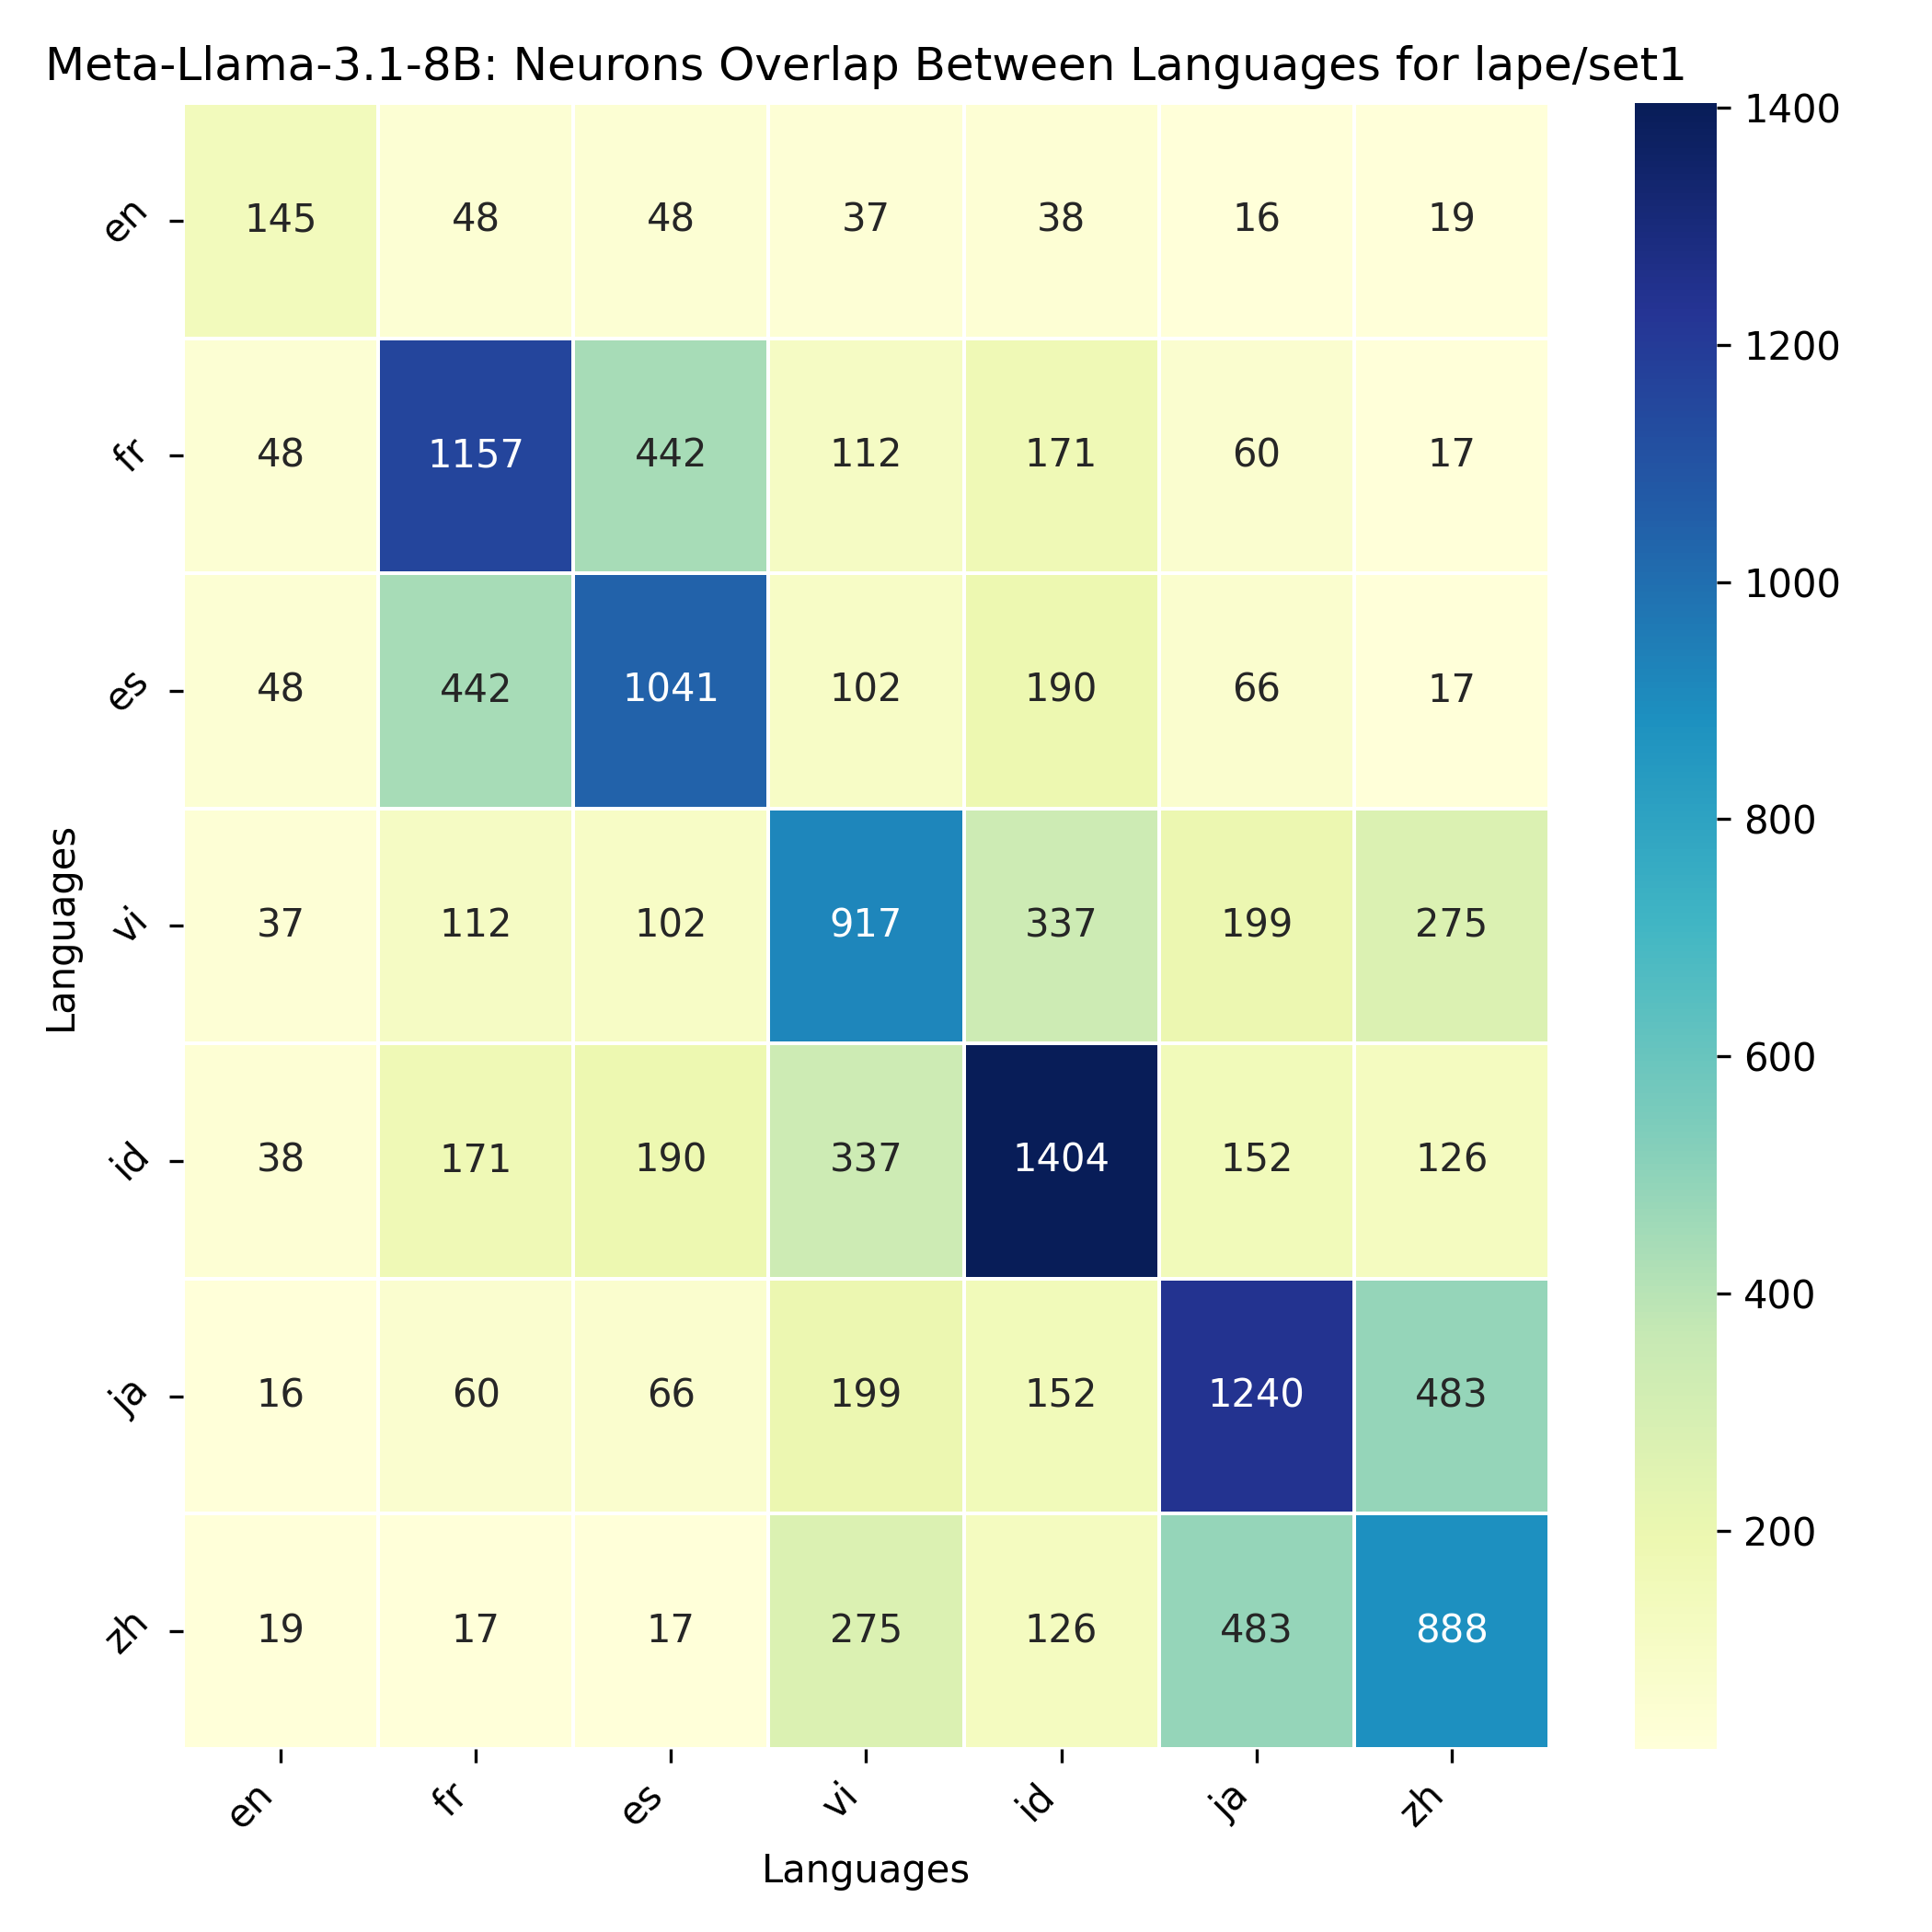
\includegraphics[width=0.45\textwidth]{Chapters/Chapter_5/lang_neurons/Meta-Llama-3.1-8B/lape/set1/lang_neurons_overlap.png} &
		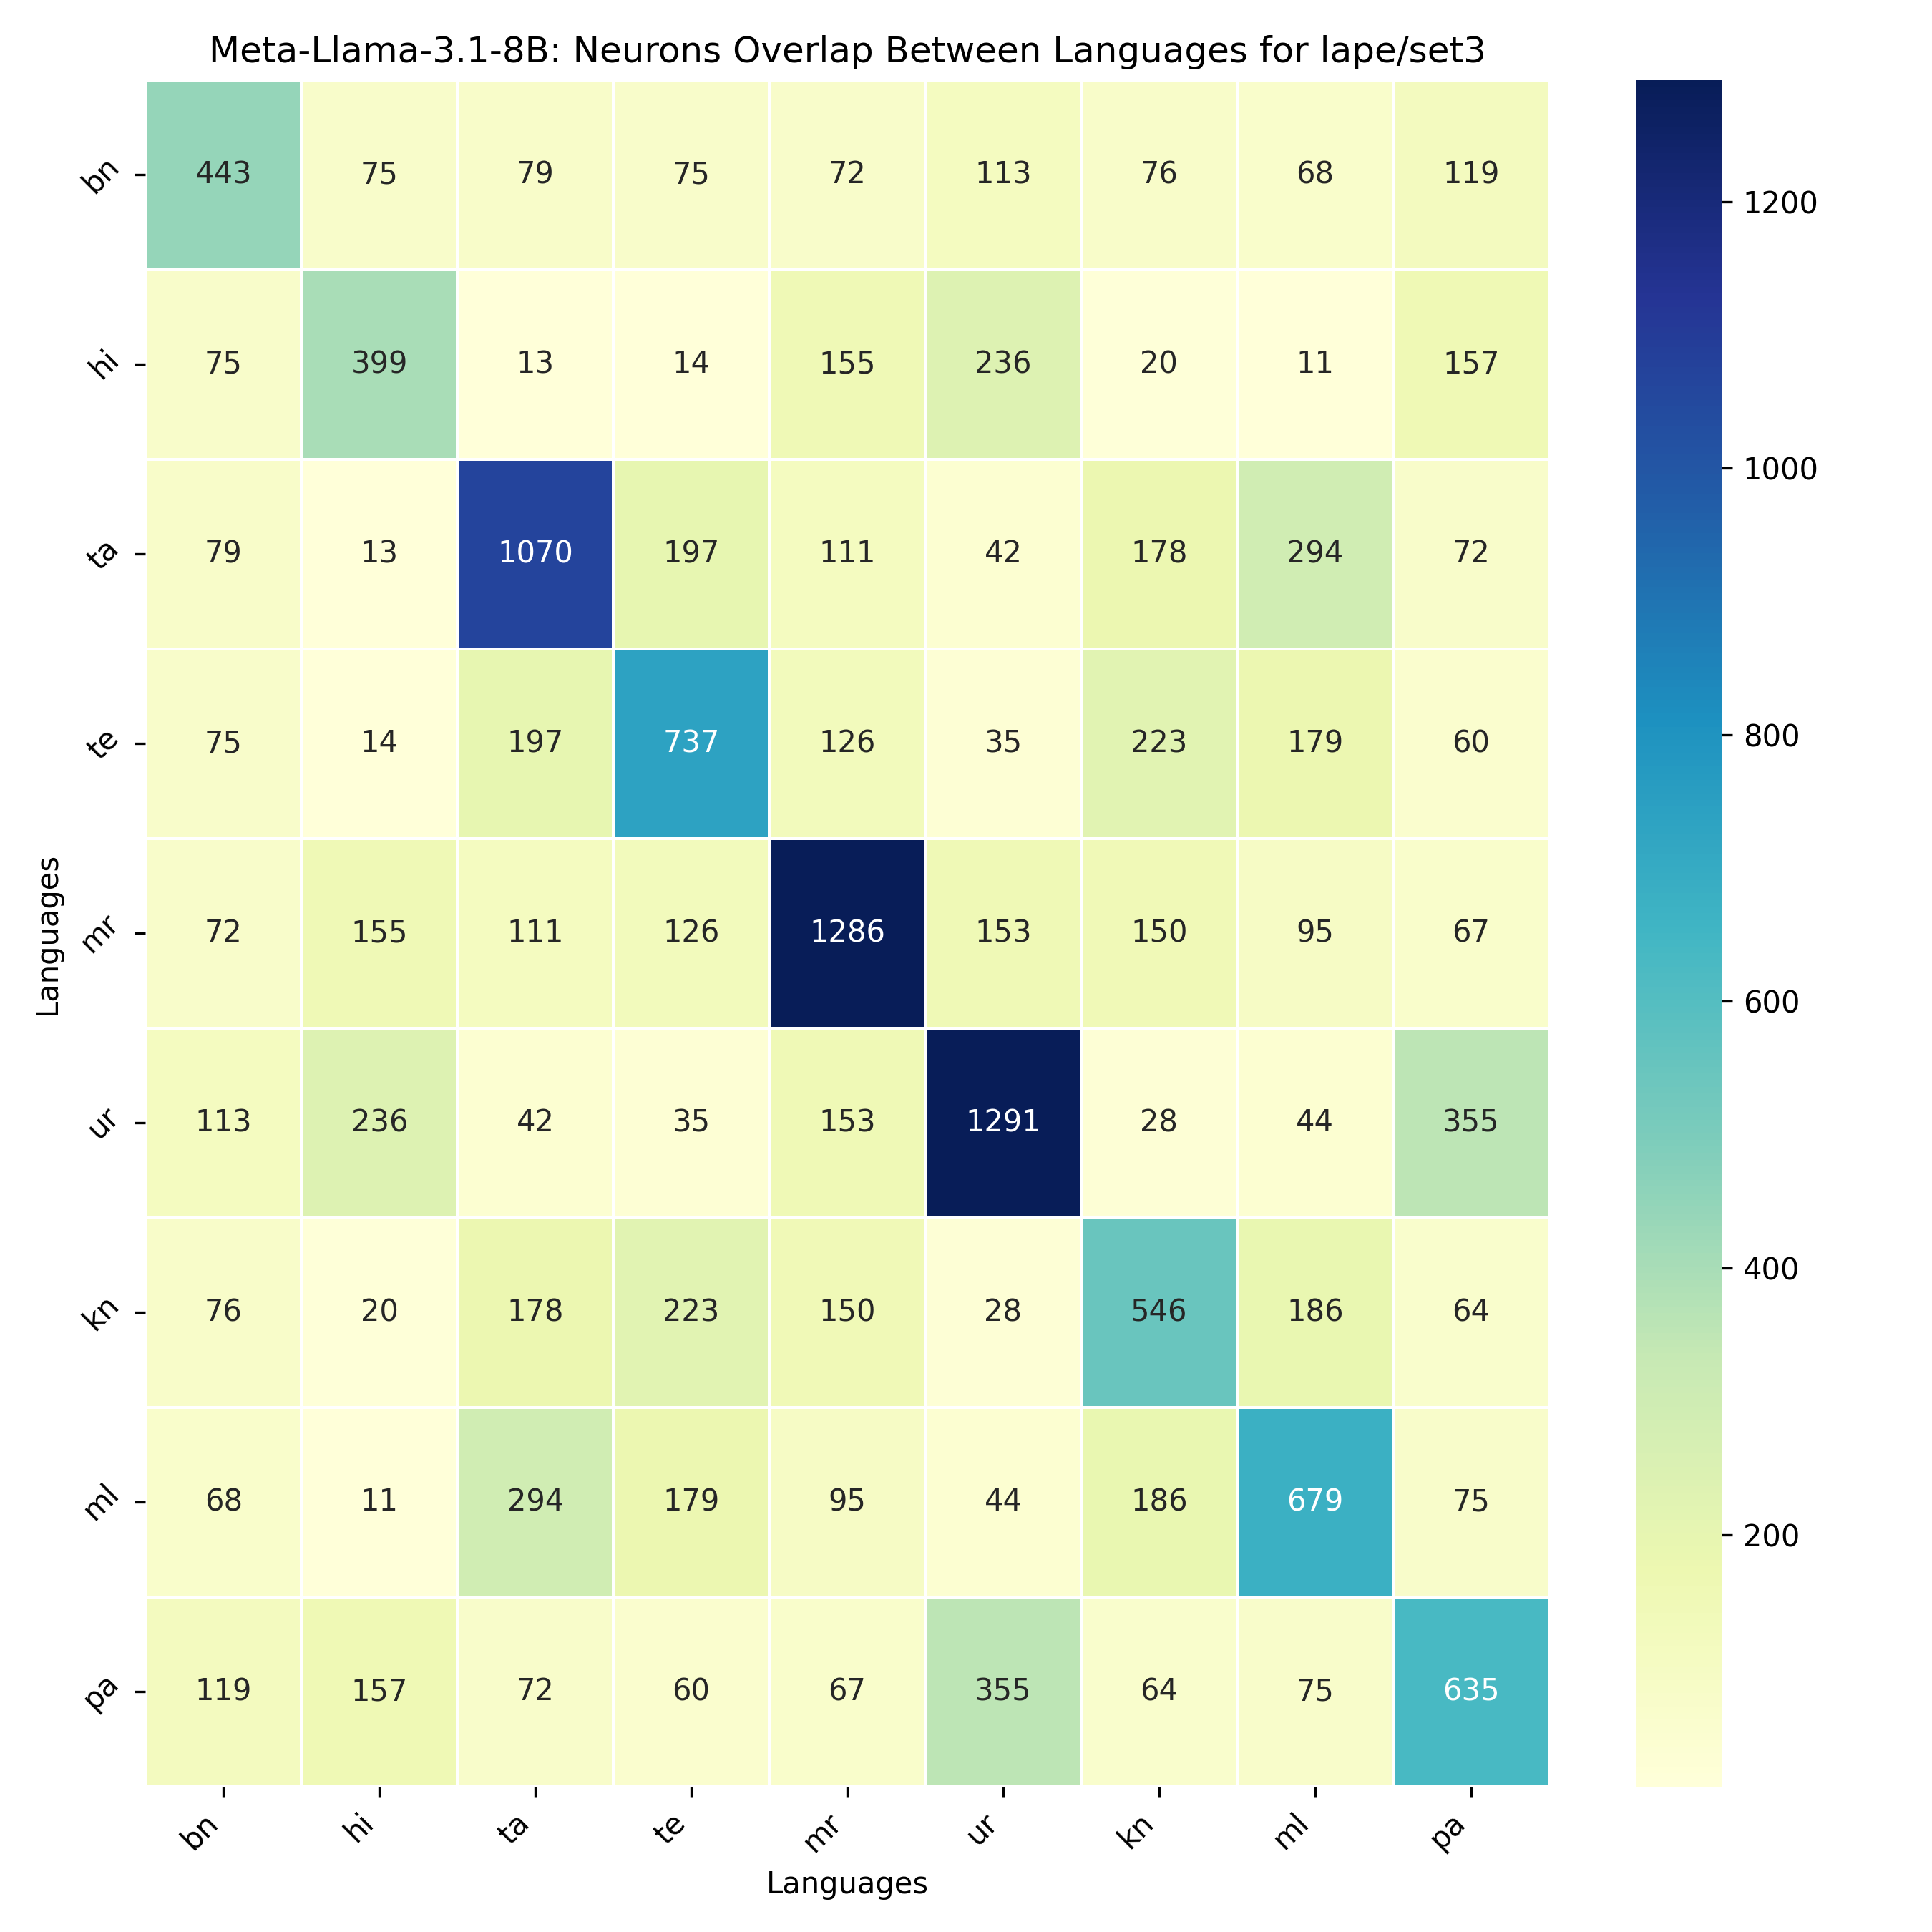
\includegraphics[width=0.45\textwidth]{Chapters/Chapter_5/lang_neurons/Meta-Llama-3.1-8B/lape/set3/lang_neurons_overlap.png} \\
		\textbf{Set1: Neuron Overlap} &
		\textbf{Set3: Neuron Overlap}
	\end{tabular}
	\caption{Neuron overlap between languages for LAPE method for Set1 and Set3.}
	\label{fig:lang_neuron_overlap}
\end{figure}

Figure \ref{fig:lang_neuron_overlap} highlights that languages with shared syntactic or morphological properties, such as \textit{id} and \textit{vi} in Set1, exhibit higher overlap. In contrast, languages like \textit{en} and \textit{fr} have minimal overlap with other languages, underscoring their unique linguistic structures.

\textbf{Layer-Wise Neuron Distribution:} The layer-wise distribution of language-specific neurons for Set1 and Set3 is shown in Figure \ref{fig:layerwise_distribution}. The distribution is computed as:
\begin{equation}
	L_l(i) = \sum_{j=1}^{4d} \mathbb{I}\left(p_{i,j}^l > \text{Threshold}\right) \cdot \delta\left((i,j) \in \text{Lang\_Set}\right),
\end{equation}
where $L_l(i)$ denotes the number of neurons in layer $i$ associated with language $l$.

\begin{figure}[ht]
	\centering
	\begin{tabular}{cc}
		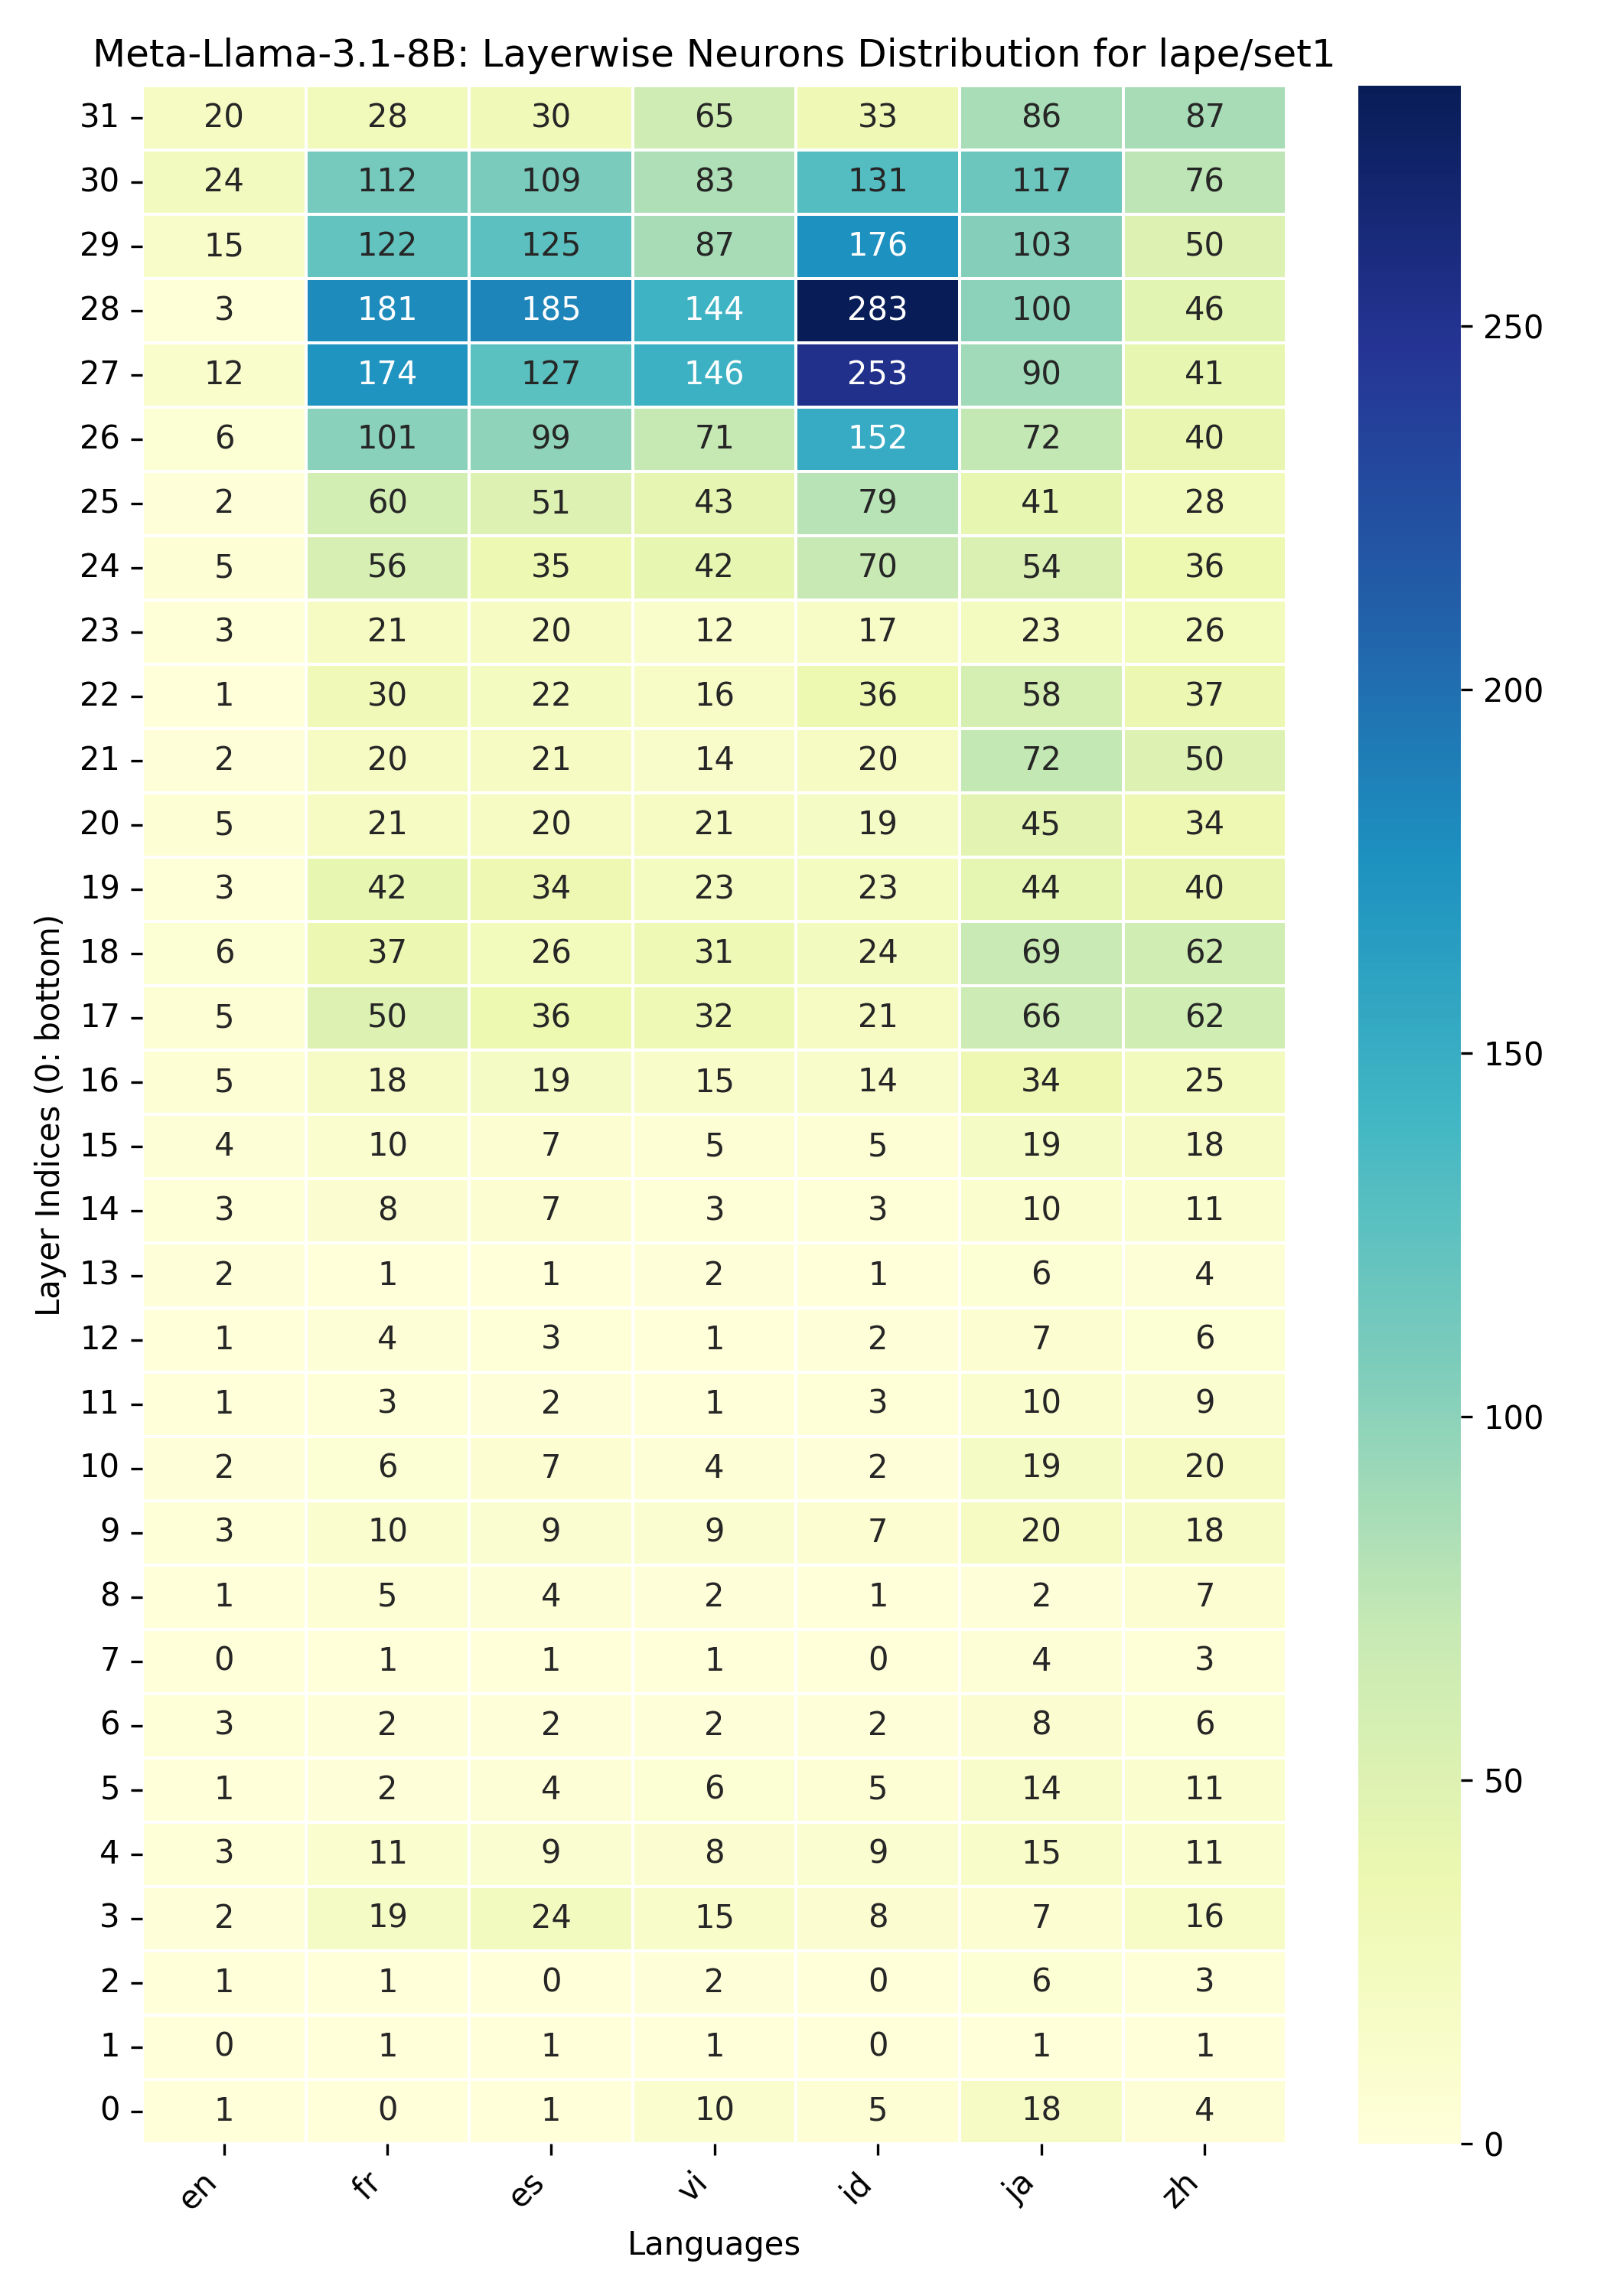
\includegraphics[width=0.45\textwidth]{Chapters/Chapter_5/lang_neurons/Meta-Llama-3.1-8B/lape/set1/layerwise_lang_neurons_dist.png} &
		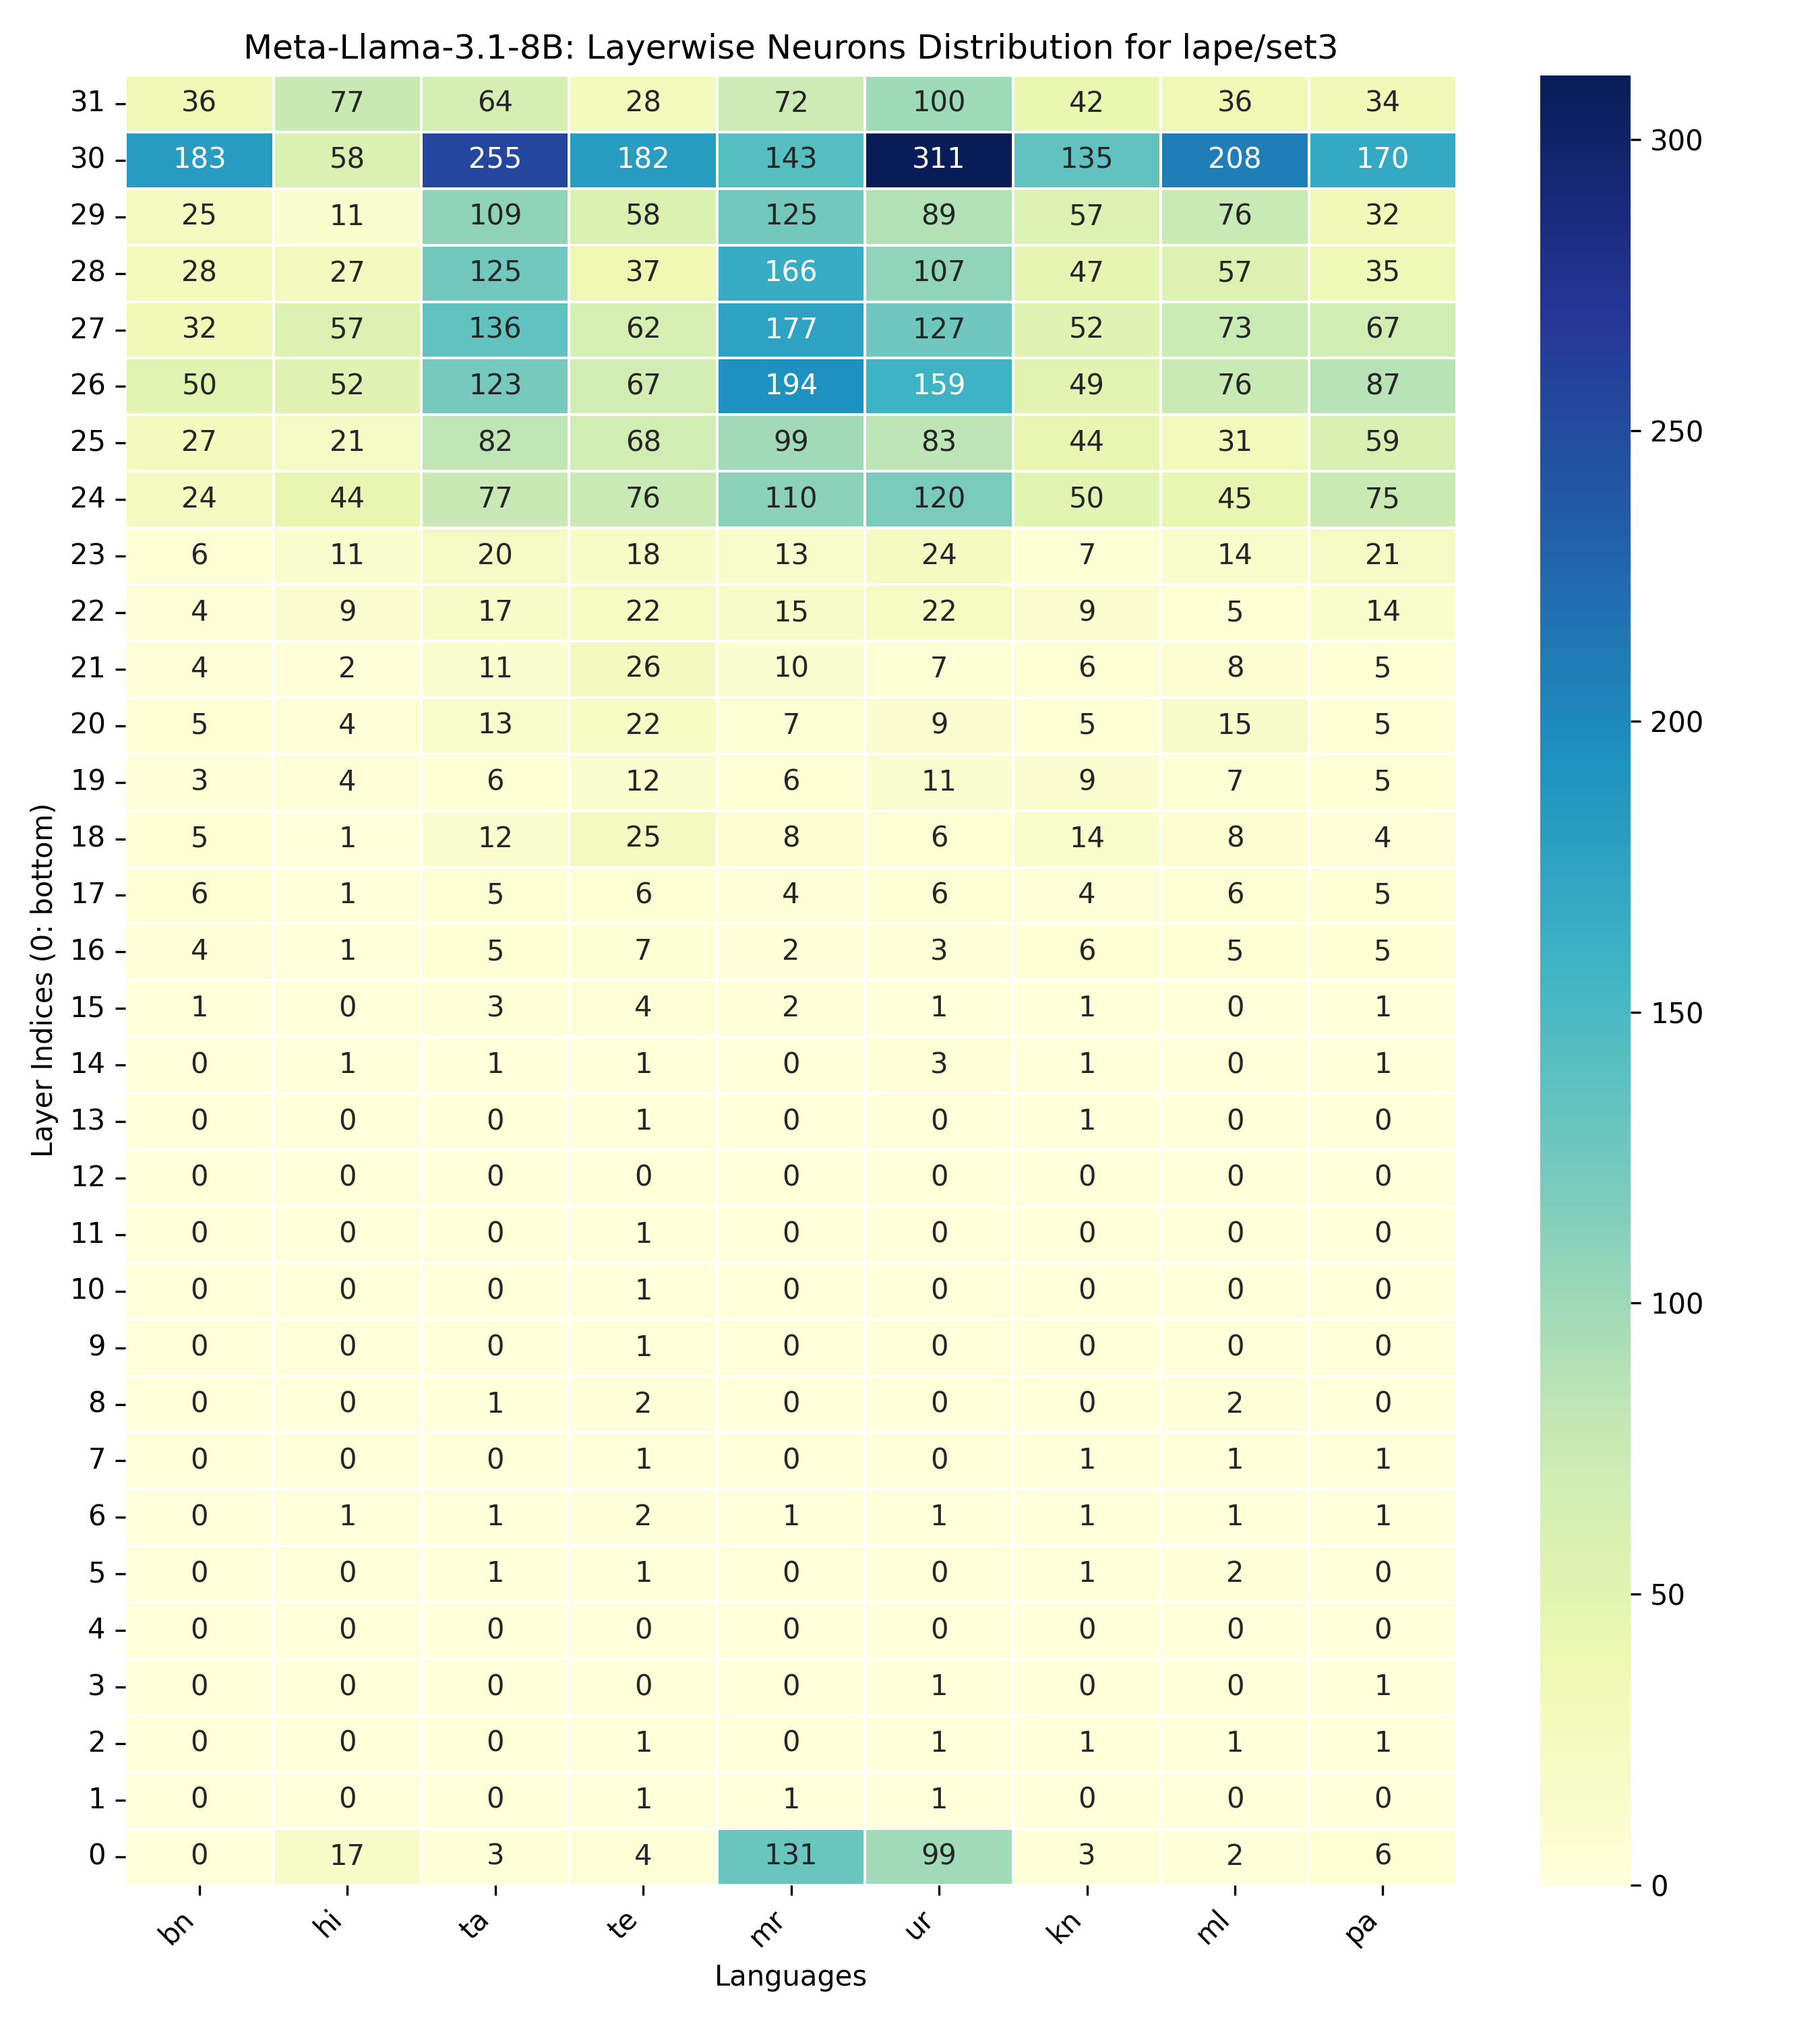
\includegraphics[width=0.45\textwidth]{Chapters/Chapter_5/lang_neurons/Meta-Llama-3.1-8B/lape/set3/layerwise_lang_neurons_dist.png} \\
		\textbf{Set1: Layer-wise Neuron Distribution} &
		\textbf{Set3: Layer-wise Neuron Distribution}
	\end{tabular}
	\caption{Layer-wise neuron distributions for LAPE method for Set1 and Set3.}
	\label{fig:layerwise_distribution}
\end{figure}

Figure \ref{fig:layerwise_distribution} reveals that language-specific neurons are concentrated in the upper layers (e.g., Layers 27-30), aligning with the notion that deeper layers capture more abstract and language-specific features. Lower layers exhibit fewer neurons, as they primarily encode shared linguistic features.

\subsection{Perplexity Change}

\textbf{Perplexity (PPX):} Perplexity is a widely used metric to evaluate the performance of language models. It measures how well a model predicts a sequence of tokens and is formally defined as the exponential of the average negative log-probability of the tokens in a sequence. 

Mathematically, for a sequence of tokens $\mathbf{x} = (x_1, x_2, \dots, x_T)$, the perplexity is given by:

\begin{equation}
	\text{PPX}(\mathbf{x}) = \exp\left(-\frac{1}{T} \sum_{t=1}^T \log P(x_t \,|\, x_{<t})\right),
\end{equation}

where:
\begin{itemize}
	\item $T$ is the length of the sequence.
	\item $P(x_t \,|\, x_{<t})$ is the probability assigned by the model to the token $x_t$, given the preceding tokens $x_{<t} = (x_1, x_2, \dots, x_{t-1})$.
\end{itemize}

Perplexity can be understood as the average branching factor of the model in predicting tokens. A lower perplexity indicates that the model is more confident in its predictions, while a higher perplexity suggests greater uncertainty.

For a dataset $\mathcal{D}$ consisting of multiple sequences, the perplexity is computed as the mean of the per-sequence perplexities:

\begin{equation}
	\text{PPX}(\mathcal{D}) = \exp\left(-\frac{1}{N} \sum_{i=1}^N \frac{1}{T_i} \sum_{t=1}^{T_i} \log P(x_t^{(i)} \,|\, x_{<t}^{(i)})\right),
\end{equation}

where $N$ is the total number of sequences in the dataset, and $T_i$ is the length of the $i$-th sequence.

\textbf{Perplexity Change (PPXC):} In the context of language modeling, perplexity serves as a key metric to measure the performance of a model. It quantifies how well a probability distribution predicts a sample. The perplexity change $\text{PPXC}(i,j)$ measures the change in perplexity for a target language $j$ when an intervention is applied at a source language $i$. Formally, it is defined as:

\begin{equation}
	\text{PPXC}(i,j) = \text{PPX}(j \,|\, \text{Intervention at } i) - \text{PPX}(j),
\end{equation}

where $\text{PPX}(j)$ denotes the original perplexity for language $j$, and $\text{PPX}(j \,|\, \text{Intervention at } i)$ is the perplexity after performing an intervention at language $i$. Lower values of $\text{PPXC}(i,j)$ indicate minimal interference, whereas higher values highlight a significant change in the model's understanding of language $j$ due to the intervention.

\textbf{Experimental Setup:} For this experiment, we used the Wikipedia dataset for each language. The experiments were conducted for two sets of languages: \textbf{Set1}, containing \{\textit{en, fr, es, vi, id, ja, zh}\}, and \textbf{Set3}, containing \{\textit{bn, hi, ta, te, mr, ur, kn, ml, pa}\}. The perplexity values were computed for each language, both with and without intervention at other languages.

\textbf{Analysis:} The Figure \ref{fig:ppx_change} illustrates the perplexity changes for Set1 and Set3. Each heatmap represents $\text{PPXC}(i,j)$ values for different combinations of source and target languages. In all the experiments, the intervention means the values for the neuron activation is set as zero.

\begin{figure}[ht]
	\centering
	\begin{tabular}{cc}
		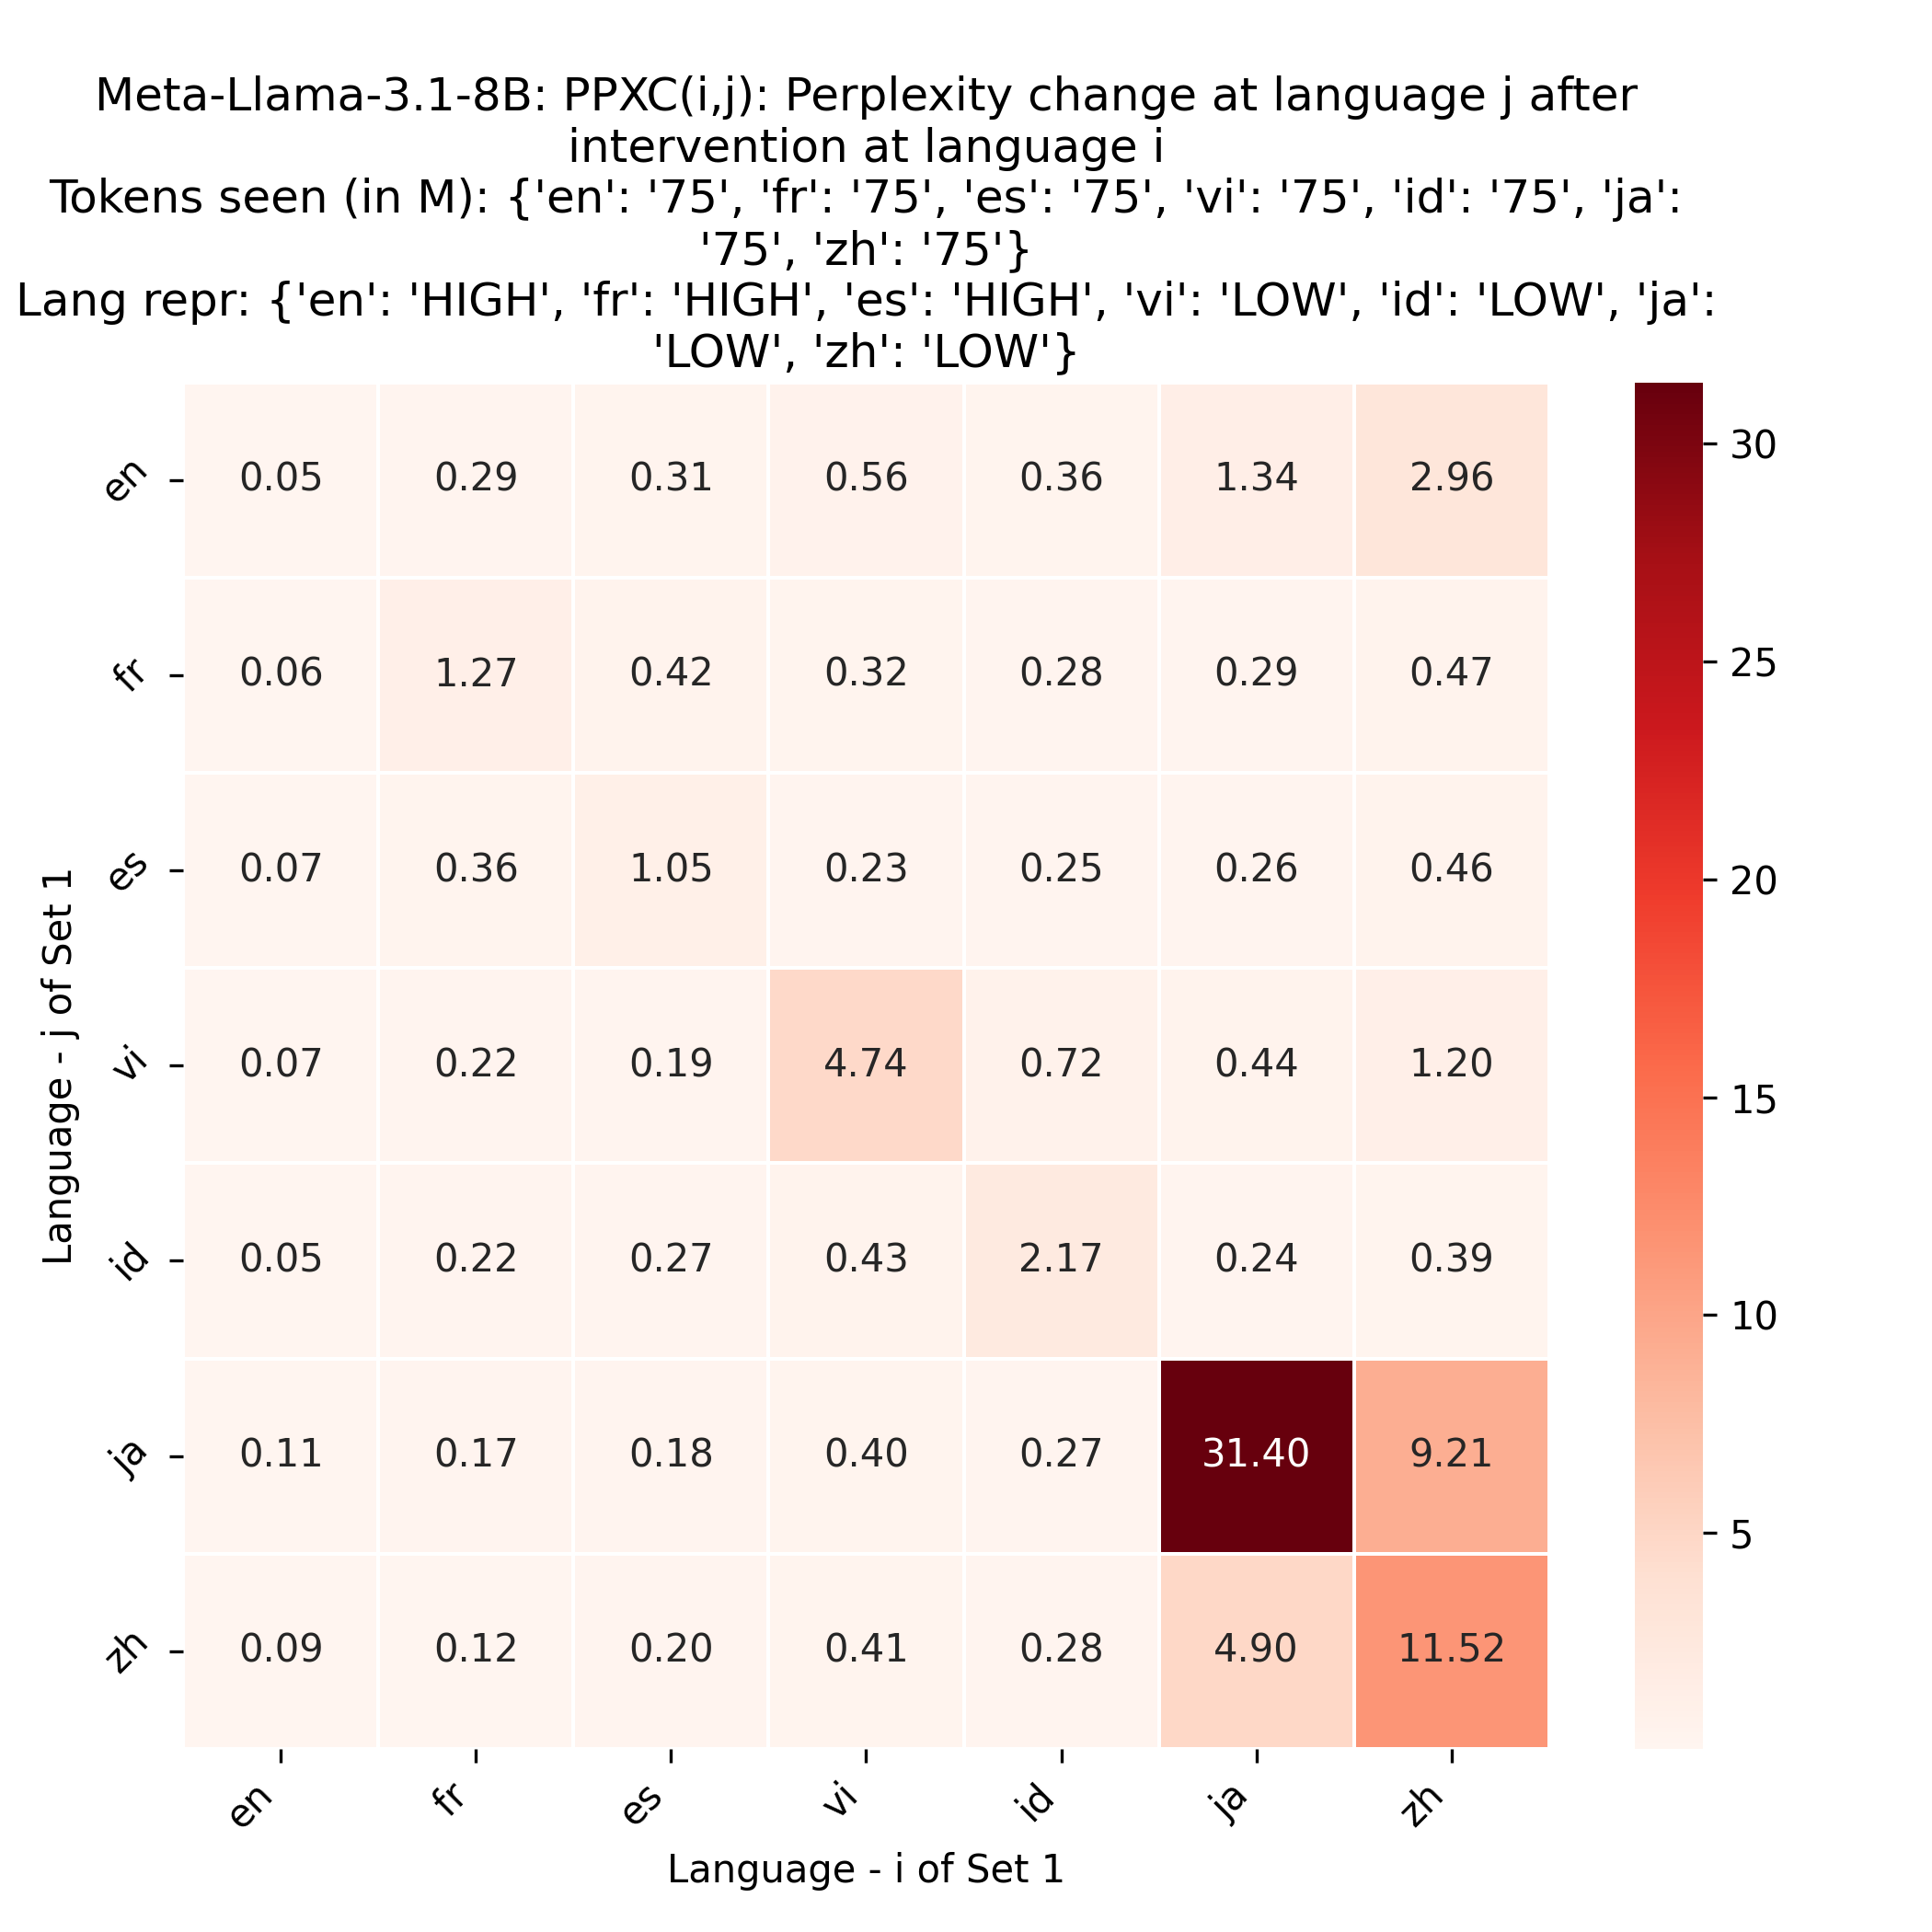
\includegraphics[width=0.45\textwidth]{Chapters/Chapter_5/perplexity/Meta-Llama-3.1-8B/set1/ppx_change.png} &
		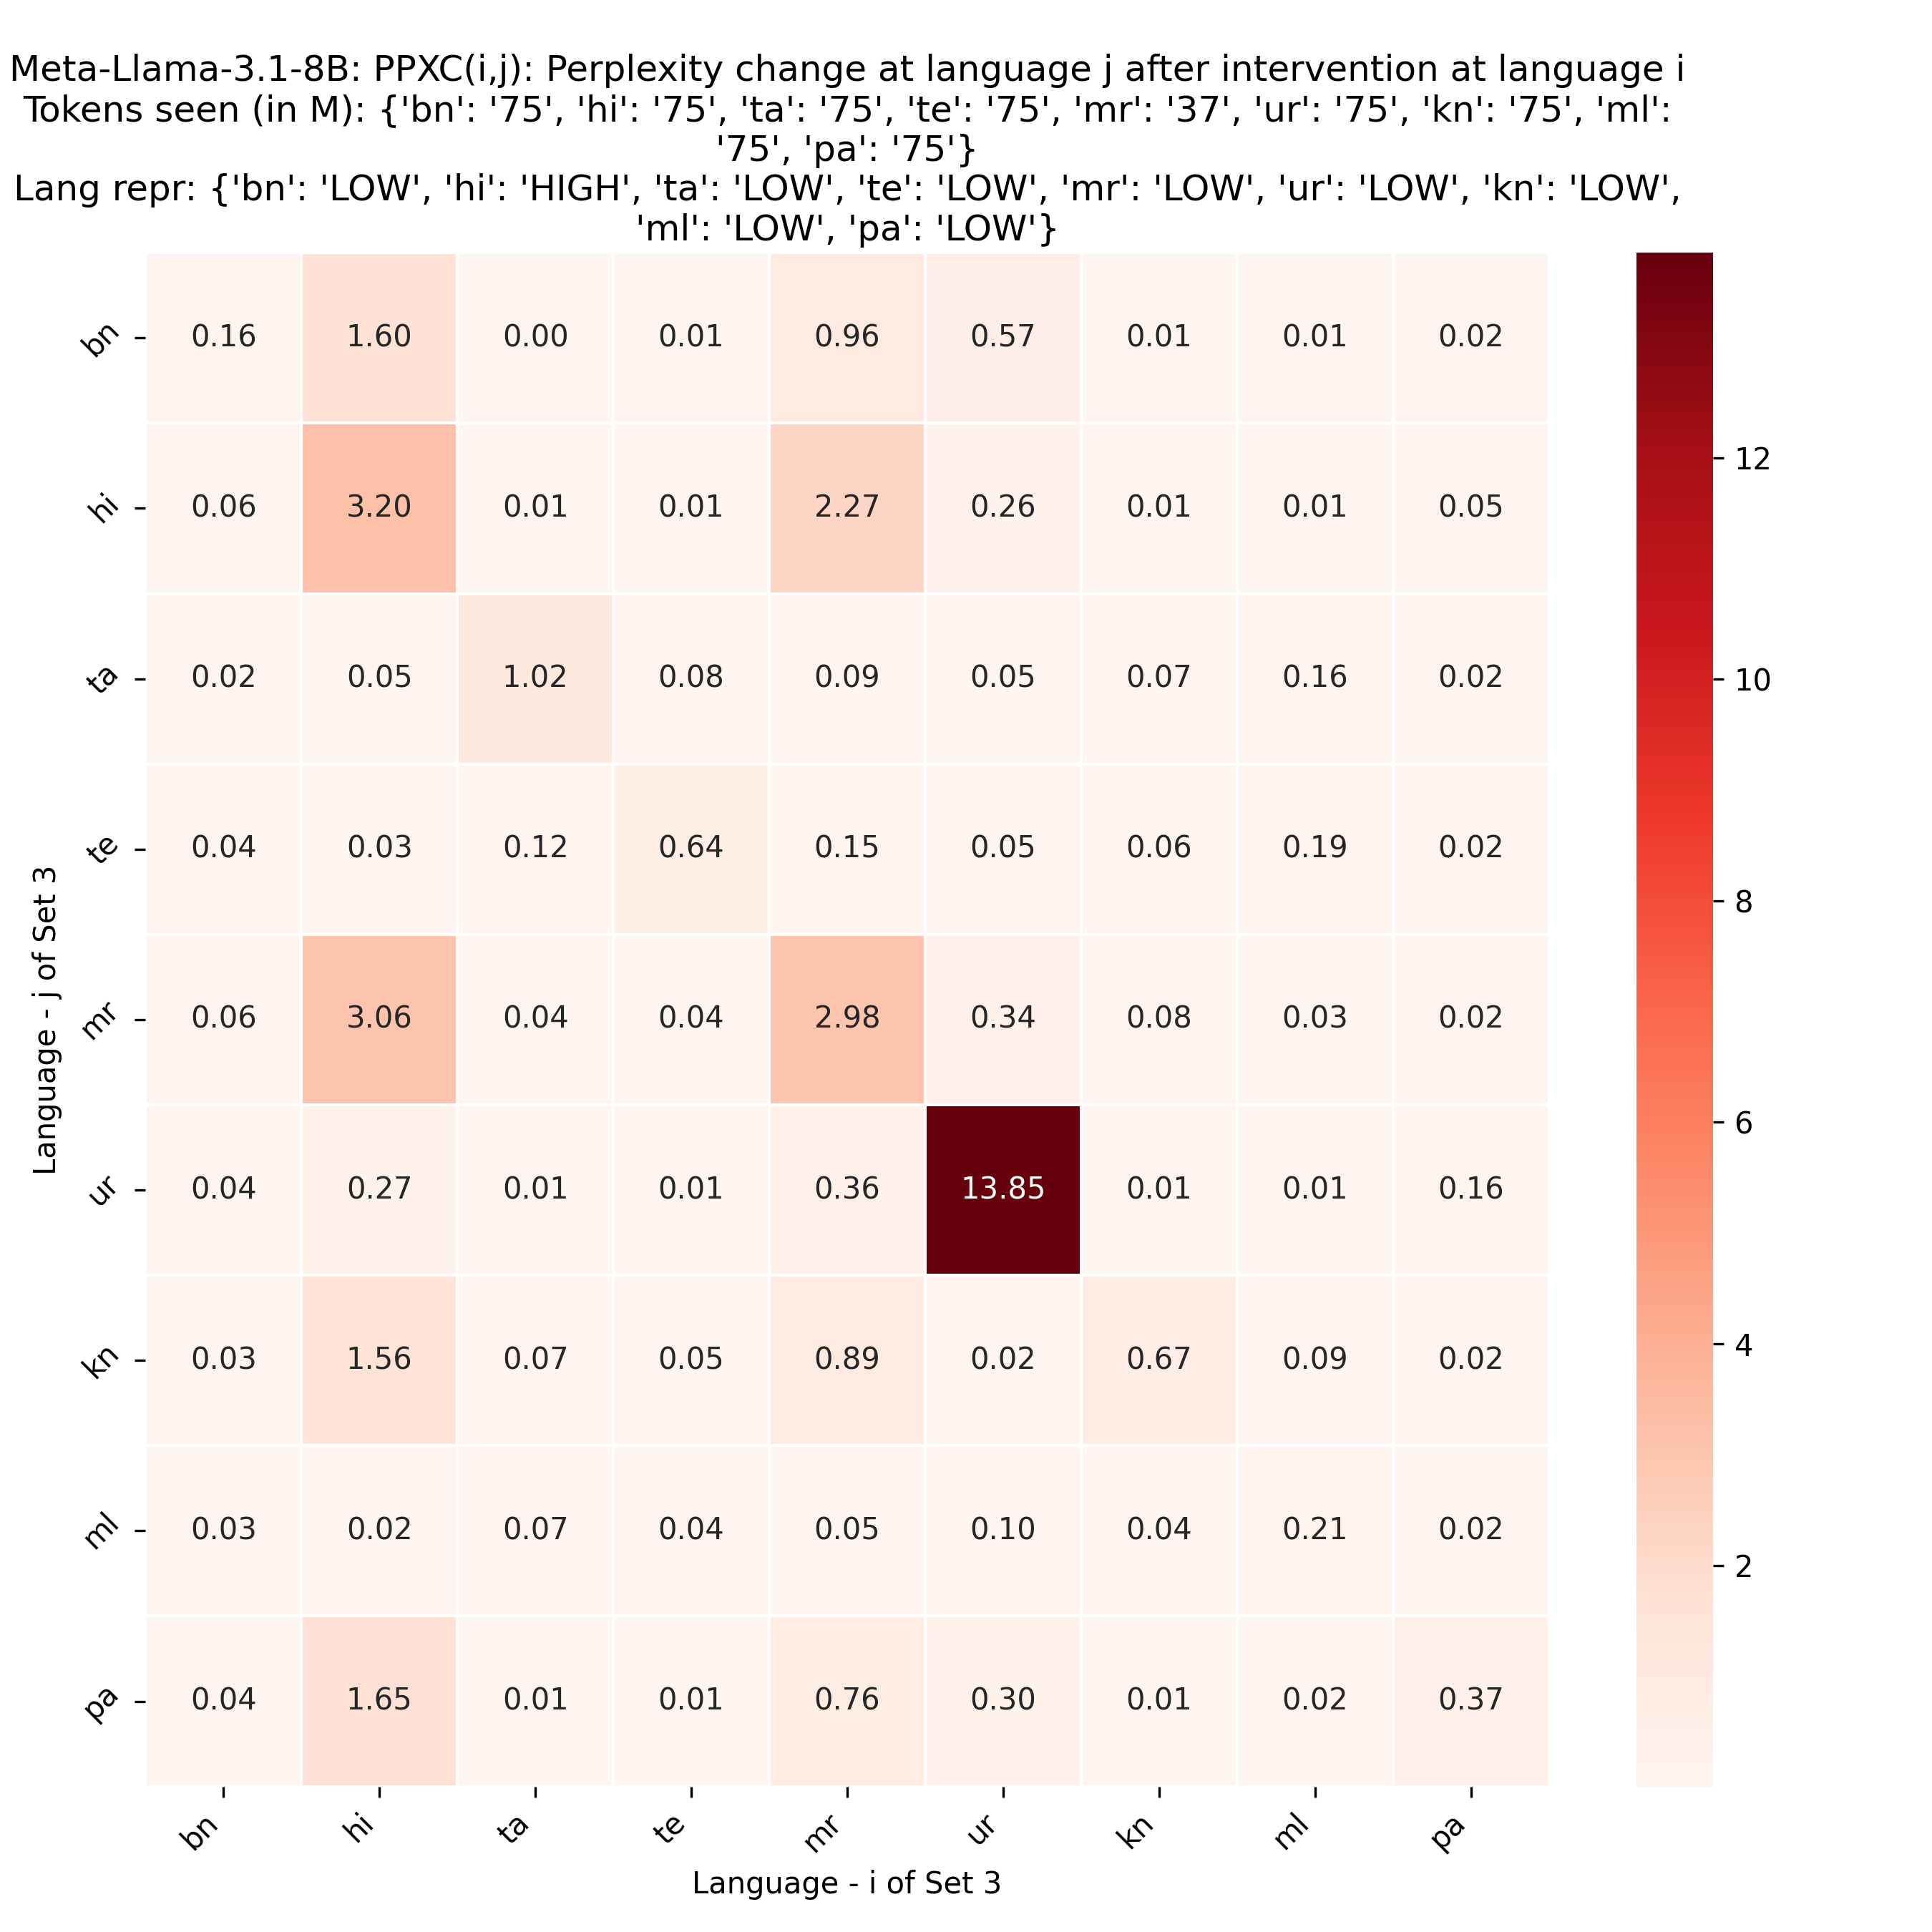
\includegraphics[width=0.45\textwidth]{Chapters/Chapter_5/perplexity/Meta-Llama-3.1-8B/set3/ppx_change.png} \\
		\textbf{Set1: Perplexity Change} &
		\textbf{Set3: Perplexity Change}
	\end{tabular}
	\caption{Perplexity change $\text{PPXC}(i,j)$ for LAPE method for Set1 and Set3.}
	\label{fig:ppx_change}
\end{figure}

From Figure \ref{fig:ppx_change}, we observe the following key trends:
\begin{itemize}
	\item For \textbf{Set1}, interventions at low-resource languages such as \textit{ja} lead to substantial perplexity changes for other low-resource languages (\textit{zh, id, vi}), as indicated by high $\text{PPXC}(i,j)$ values. This suggests that these languages share overlapping representations in the model.
	\item For \textbf{Set3}, interventions at \textit{ur} result in significant perplexity changes for other low-resource languages like \textit{ta, te}, highlighting the influence of high-representation languages on their low-representation counterparts.
\end{itemize}

\subsection{XNLI Task Results After Targeted Neurons Fine-Tuning}

Table~\ref{tab:xnli_results} summarizes the results of the fine-tuning experiments on the XNLI task. These experiments involve evaluating the zero-shot performance of the model on Vietnamese (\textit{vi}), Hindi (\textit{hi}), and Urdu (\textit{ur}) after targeted neuron fine-tuning and statistical interventions. The table reports the results (\textit{No Int}) alongside the effects of interventions using statistical patterns (\textit{Mean}, P75, P90, and P95).

\textbf{Insights from Results:}
\begin{itemize}
	\item \textbf{No Intervention Performance:} The model (\textit{No Int}) achieves robust zero-shot performance for all three languages. For instance, in \textit{vi}, the baseline accuracy is highest (0.8053) with no fine-tuning of neurons.
	\item \textbf{Impact of Interventions:} Statistical interventions generally degrade the model's performance. The degradation becomes more significant with higher percentiles (e.g., P90 and P95), indicating that extreme activation values may negatively affect generalization.
	\item \textbf{Language-Specific Trends:} For \textit{ur}, fine-tuning both English and Urdu neurons (\textit{set6\_en + ur}) shows marginal improvement in baseline performance compared to other setups. However, statistical interventions still result in performance drops.
	\item \textbf{Fine-Tuning Trade-Offs:} Fine-tuning neurons specific to the target language (\textit{set1\_vi, set6\_hi, set6\_ur}) offers better specialization for the target language. However, this comes at the cost of reduced generalization, as seen in the reduced accuracy for higher percentiles.
\end{itemize}

\begin{table}[ht]
	\centering
	\renewcommand{\arraystretch}{1.3}
	\setlength{\tabcolsep}{4pt}
	\begin{tabularx}{\textwidth}{|X|X|X|X|X|X|X|}
		\hline
		\textbf{Fine-tune Neurons} & \textbf{Eval Lang} & \textbf{No Int} & \textbf{Int by $\mu$} & \textbf{Int by P75} & \textbf{Int by P90} & \textbf{Int by P95} \\
		\hline
		null & vi & 0.8053 & 0.7955 & 0.7915 & 0.7903 & 0.7897 \\
		set1\_en & vi & 0.8017 & 0.7957 & 0.7867 & 0.7847 & 0.7847 \\
		set1\_vi & vi & 0.8007 & 0.7951 & 0.7881 & 0.7855 & 0.7845 \\
		set1\_en+vi & vi & 0.8009 & 0.7943 & 0.7865 & 0.7845 & 0.7833 \\
		\hline
		null & hi & 0.7501 & 0.7521 & 0.7496 & 0.7499 & 0.7506 \\
		set1\_en & hi & 0.7476 & 0.7456 & 0.7454 & 0.7448 & 0.7434 \\
		set6\_en & hi & 0.7491 & 0.7456 & 0.7464 & 0.7458 & 0.7441 \\
		set6\_hi & hi & 0.7492 & 0.7456 & 0.7461 & 0.7448 & 0.7431 \\
		set6\_en+hi & hi & 0.7488 & 0.7448 & 0.7451 & 0.7446 & 0.7431 \\
		\hline
		null & ur & 0.7002 & 0.7044 & 0.7028 & 0.6938 & 0.6904 \\
		set6\_en & ur & 0.6984 & 0.7041 & 0.7026 & 0.6964 & 0.6923 \\
		set6\_ur & ur & 0.6984 & 0.7054 & 0.7024 & 0.6952 & 0.6913 \\
		set6\_en+ur & ur & 0.6992 & 0.7061 & 0.7021 & 0.6954 & 0.6919 \\
		\hline
	\end{tabularx}
	\caption{XNLI task results after targeted neurons fine-tuning for LAPE method. The training language is always English.}
	\label{tab:xnli_results}
\end{table}

The results highlight the complexities of fine-tuning specific neurons for multilingual tasks. While targeted fine-tuning can improve certain aspects of language specialization, it often comes at the cost of generalization.


















\section{Activation Probability 90p Experiments}

\subsection{Language Neuron Distribution}

In this section, we analyze the distribution of language-specific neurons across the selected languages: \textit{en}, \textit{vi}, \textit{hi}, and \textit{ur}. Unlike LAPE, this approach is set-independent, meaning the results remain consistent regardless of the set of languages considered. Each language has the same number of neurons, precisely 573, allocated based on 0.0125\% of the total number of neurons. This ensures fairness and uniformity in the analysis across different languages. The emphasis here is on examining the overlap and layer-wise distribution of these neurons. The overlap matrix, as shown in Figure~\ref{fig:combined_lang_neurons}, highlights the extent to which neurons are shared between languages. This indicates that while there is some degree of shared representation, the neurons largely retain their language specificity.

The layer-wise neuron distribution, depicted in Figure~\ref{fig:combined_lang_neurons}, provides insights into the depth at which language-specific features are encoded. For all languages, a significant concentration of neurons is observed in the lower layers (e.g., Layers 4–8). This suggests that fundamental linguistic features, such as syntax and basic semantics, are predominantly captured in the initial layers. In contrast, the middle and upper layers contain fewer language-specific neurons, indicating that these layers might focus more on higher-level abstractions or tasks that are less language-dependent.


\begin{figure}[ht]
	\centering
	\begin{tabular}{cc}
		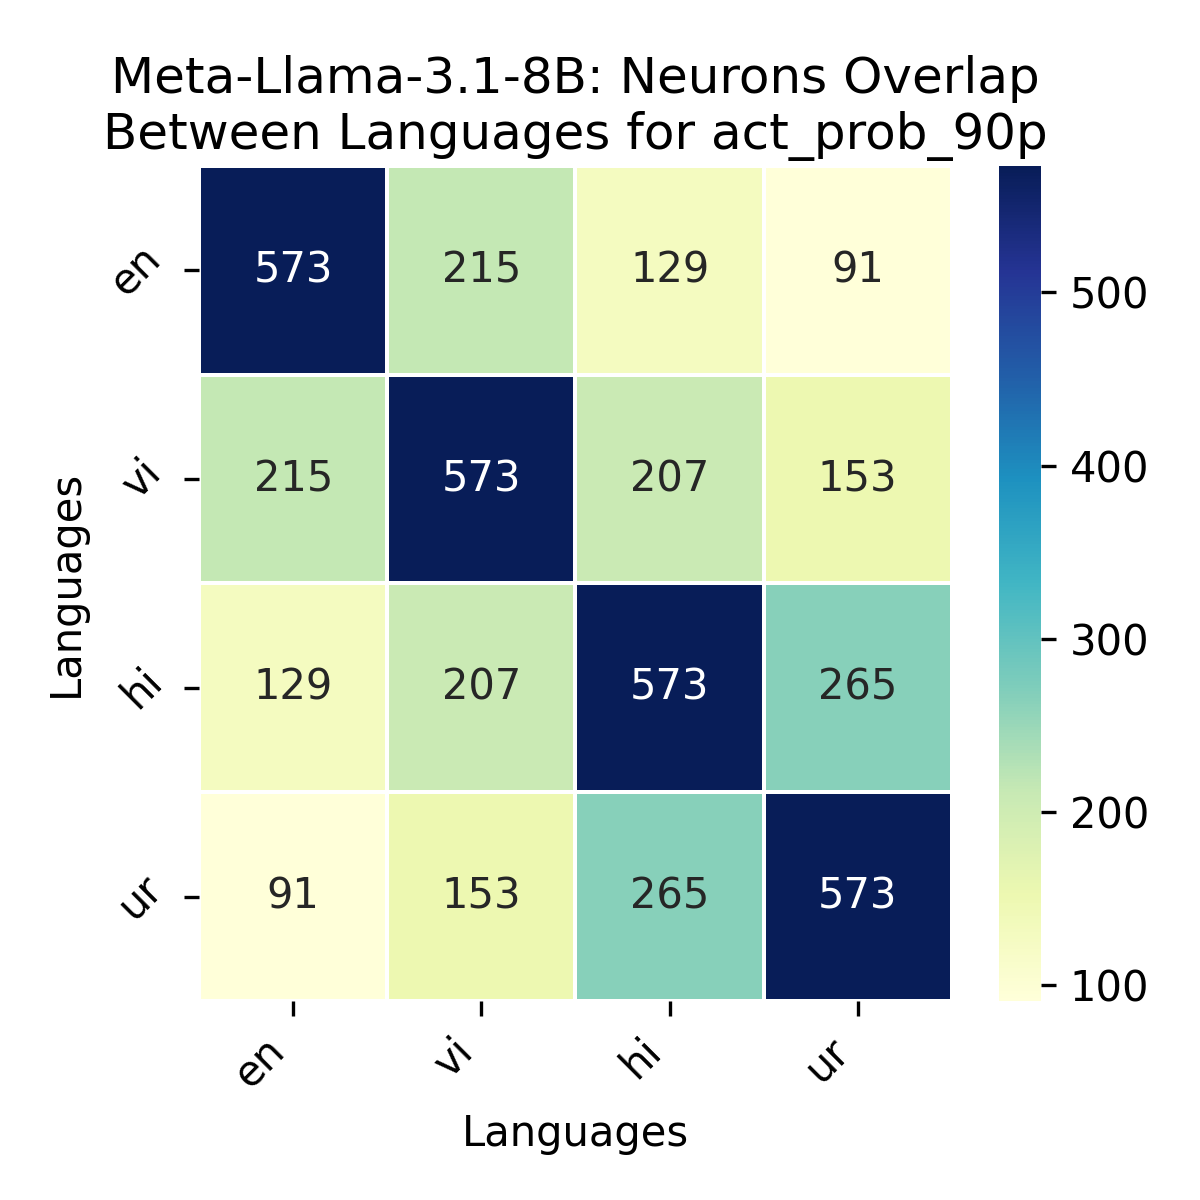
\includegraphics[width=0.60\textwidth]{Chapters/Chapter_5/lang_neurons/Meta-Llama-3.1-8B/act_prob_90p/lang_neurons_overlap.png} &
		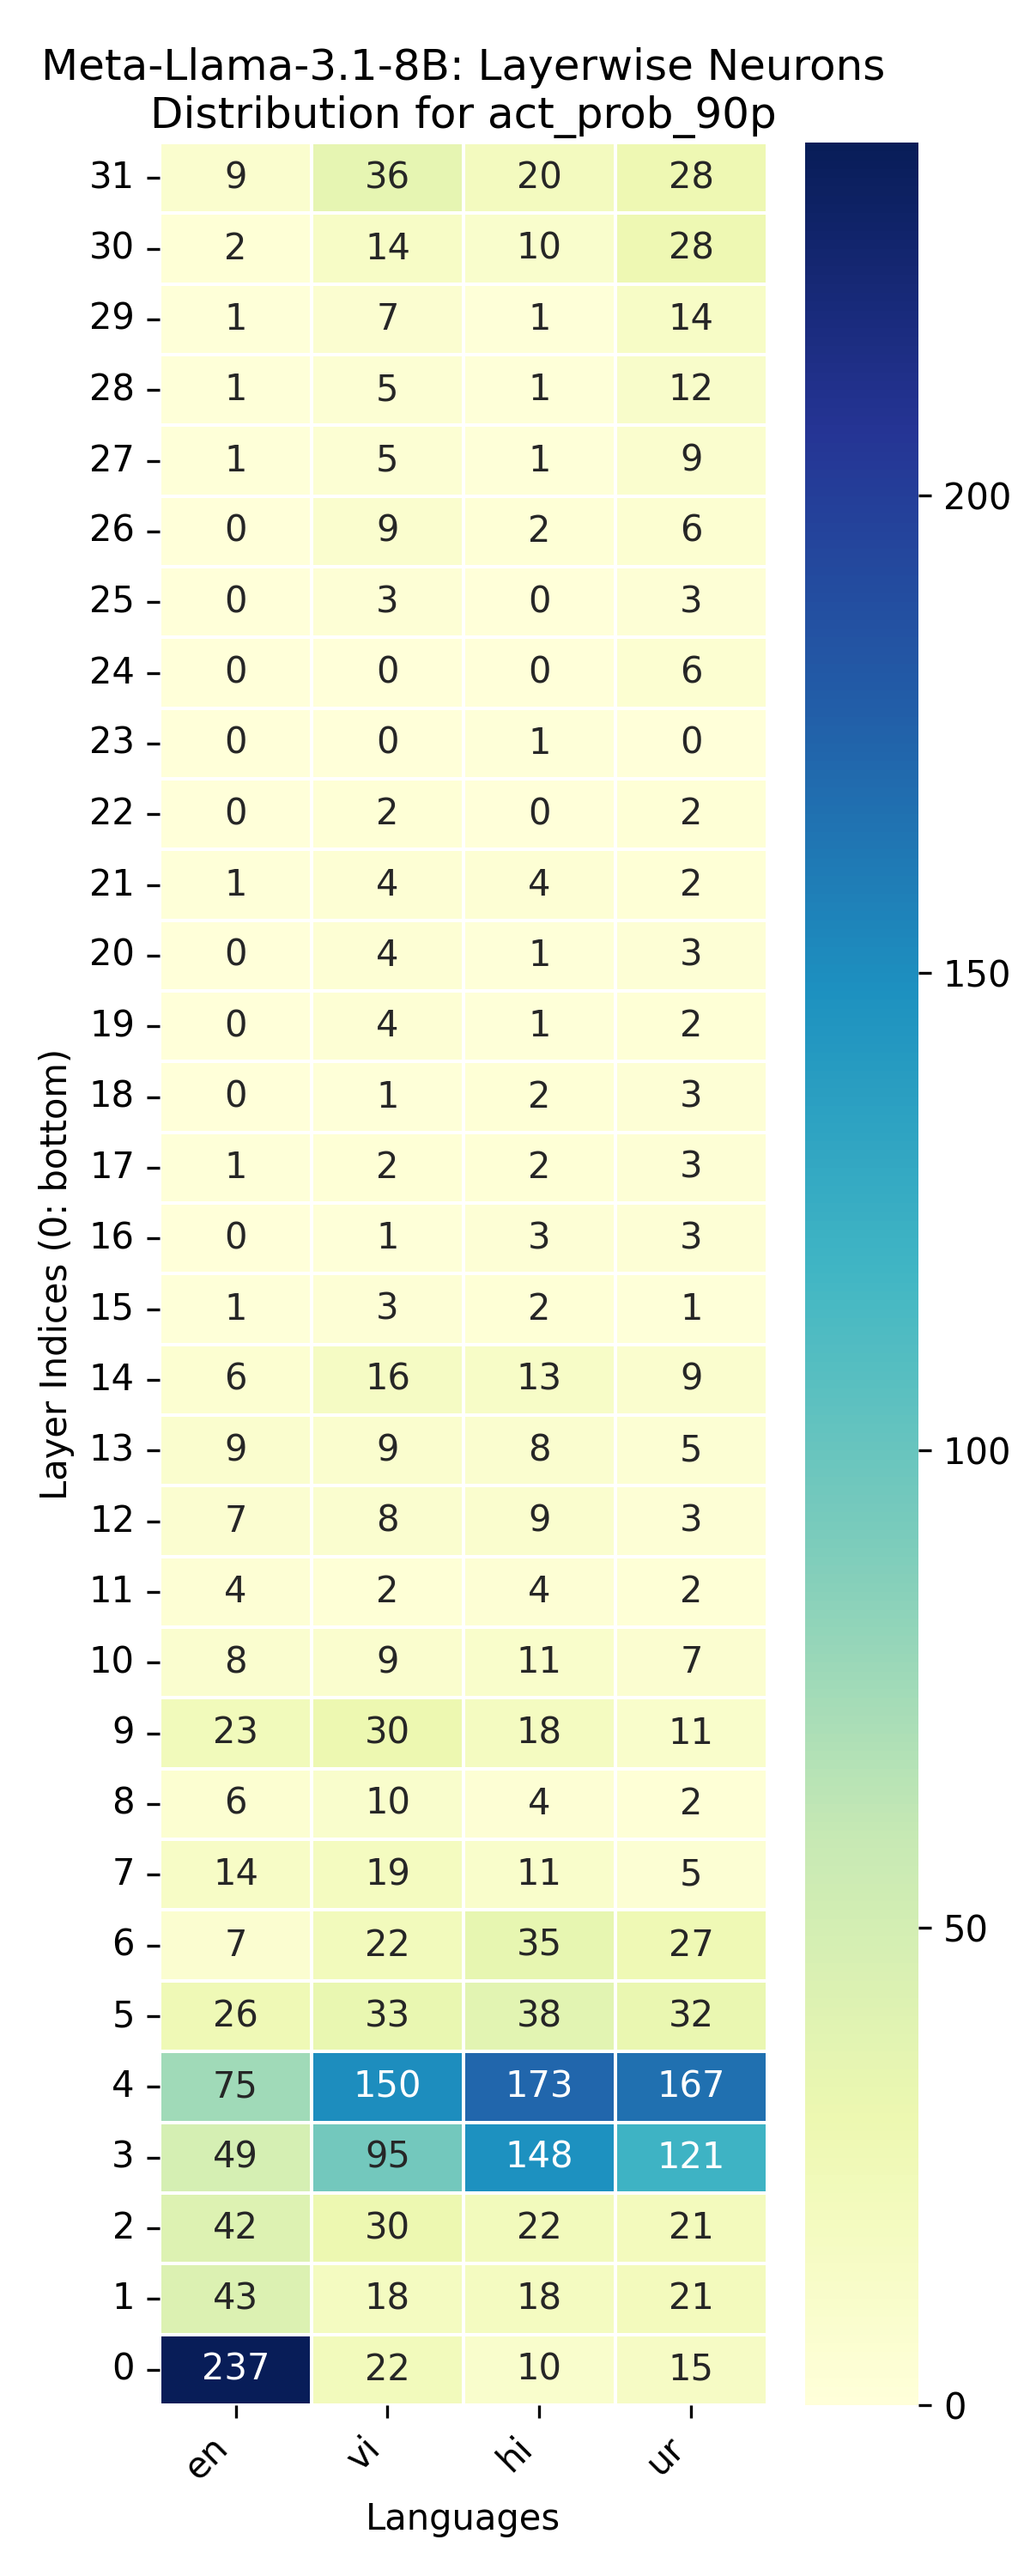
\includegraphics[width=0.30\textwidth]{Chapters/Chapter_5/lang_neurons/Meta-Llama-3.1-8B/act_prob_90p/layerwise_lang_neurons_dist.png} \\
		\textbf{Overlap Between Neurons} &
		\textbf{Layer-wise Neuron Dist}
	\end{tabular}
	\caption{Overlap between neurons and layer-wise neurons distribution for activation probability 90p method.}
	\label{fig:combined_lang_neurons}
\end{figure}


This method demonstrates a significant advantage over LAPE as it ensures consistency and fairness across languages. Since the language-specific neurons are determined independently of the set of languages considered, the analysis does not suffer from the set-dependent biases inherent in LAPE.

\subsection{Perplexity Change}

The experimental results for the perplexity change (\textit{PPXC}) are presented in this section. These results focus on analyzing the impact of interventions at one language (\textit{i}) on the perplexity of another language (\textit{j}) within the same experimental setup. The datasets used for these computations are derived from the Wikipedia corpus for the respective languages.

\begin{figure}[ht]
	\centering
	\begin{tabular}{cc}
		% First Figure: act_prob_zero
		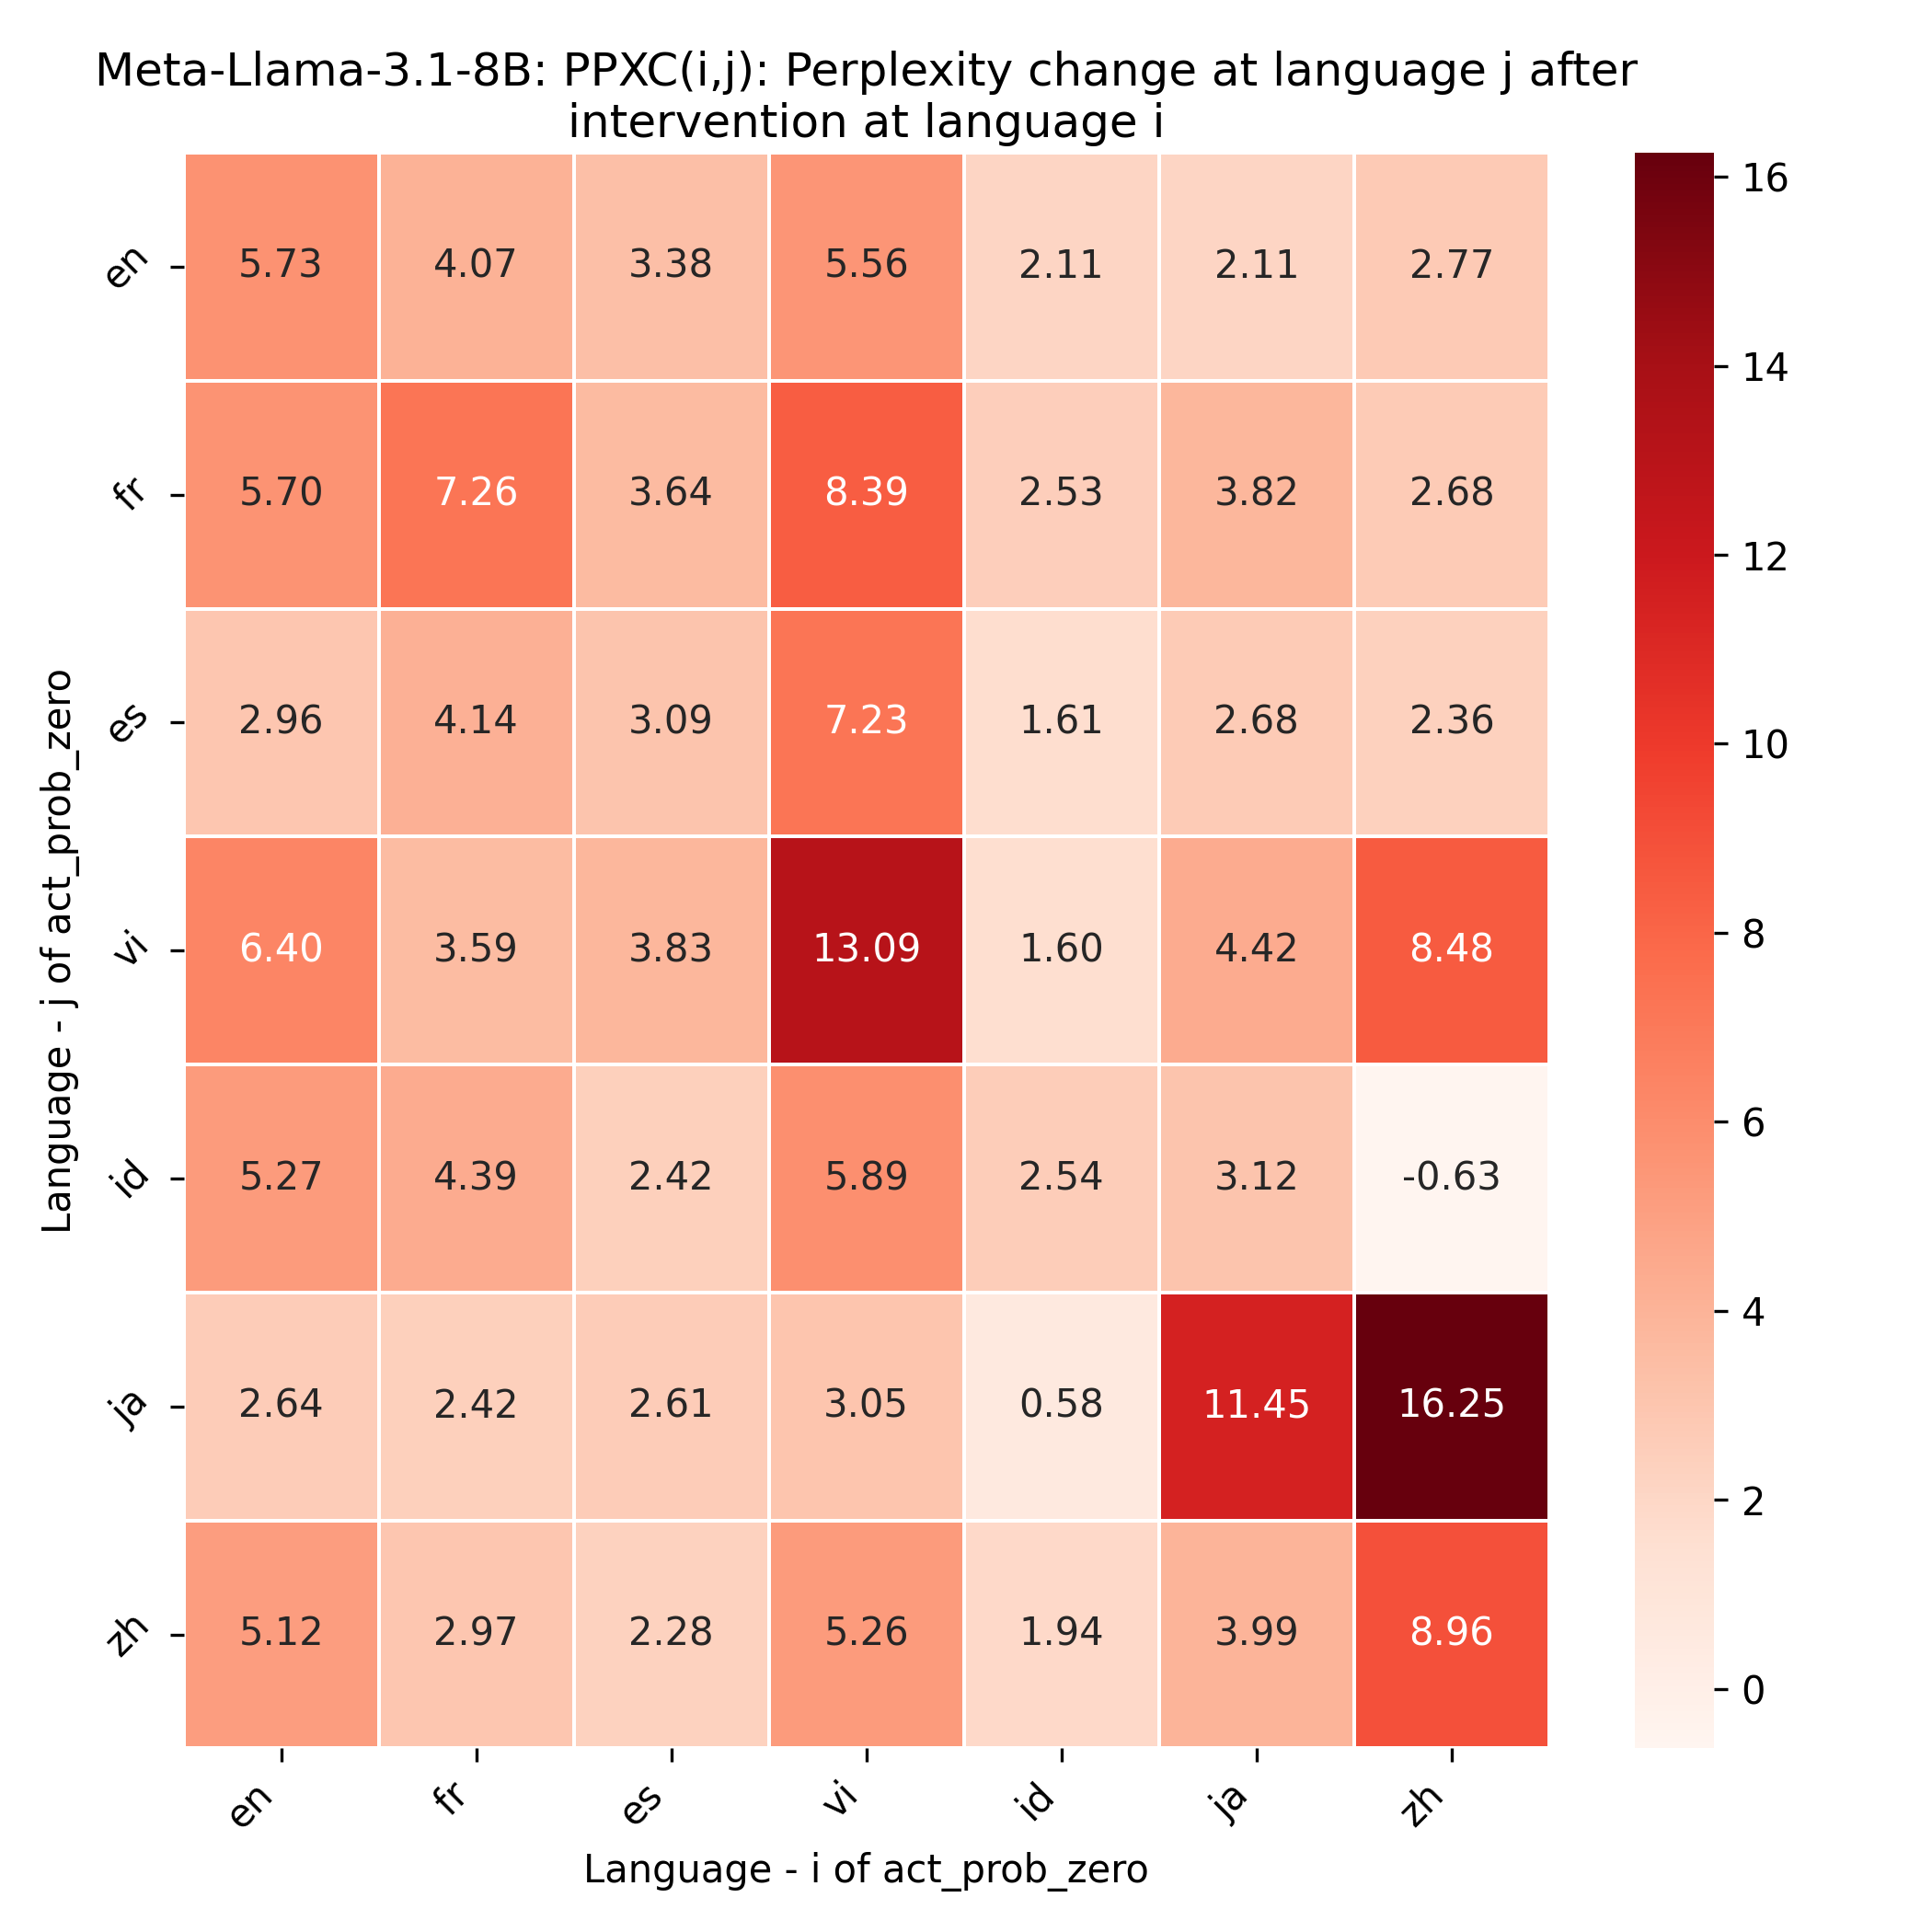
\includegraphics[width=0.45\textwidth]{Chapters/Chapter_5/perplexity/Meta-Llama-3.1-8B/act_prob_zero/ppx_change.png} &
		% Second Figure: act_prob_90p
		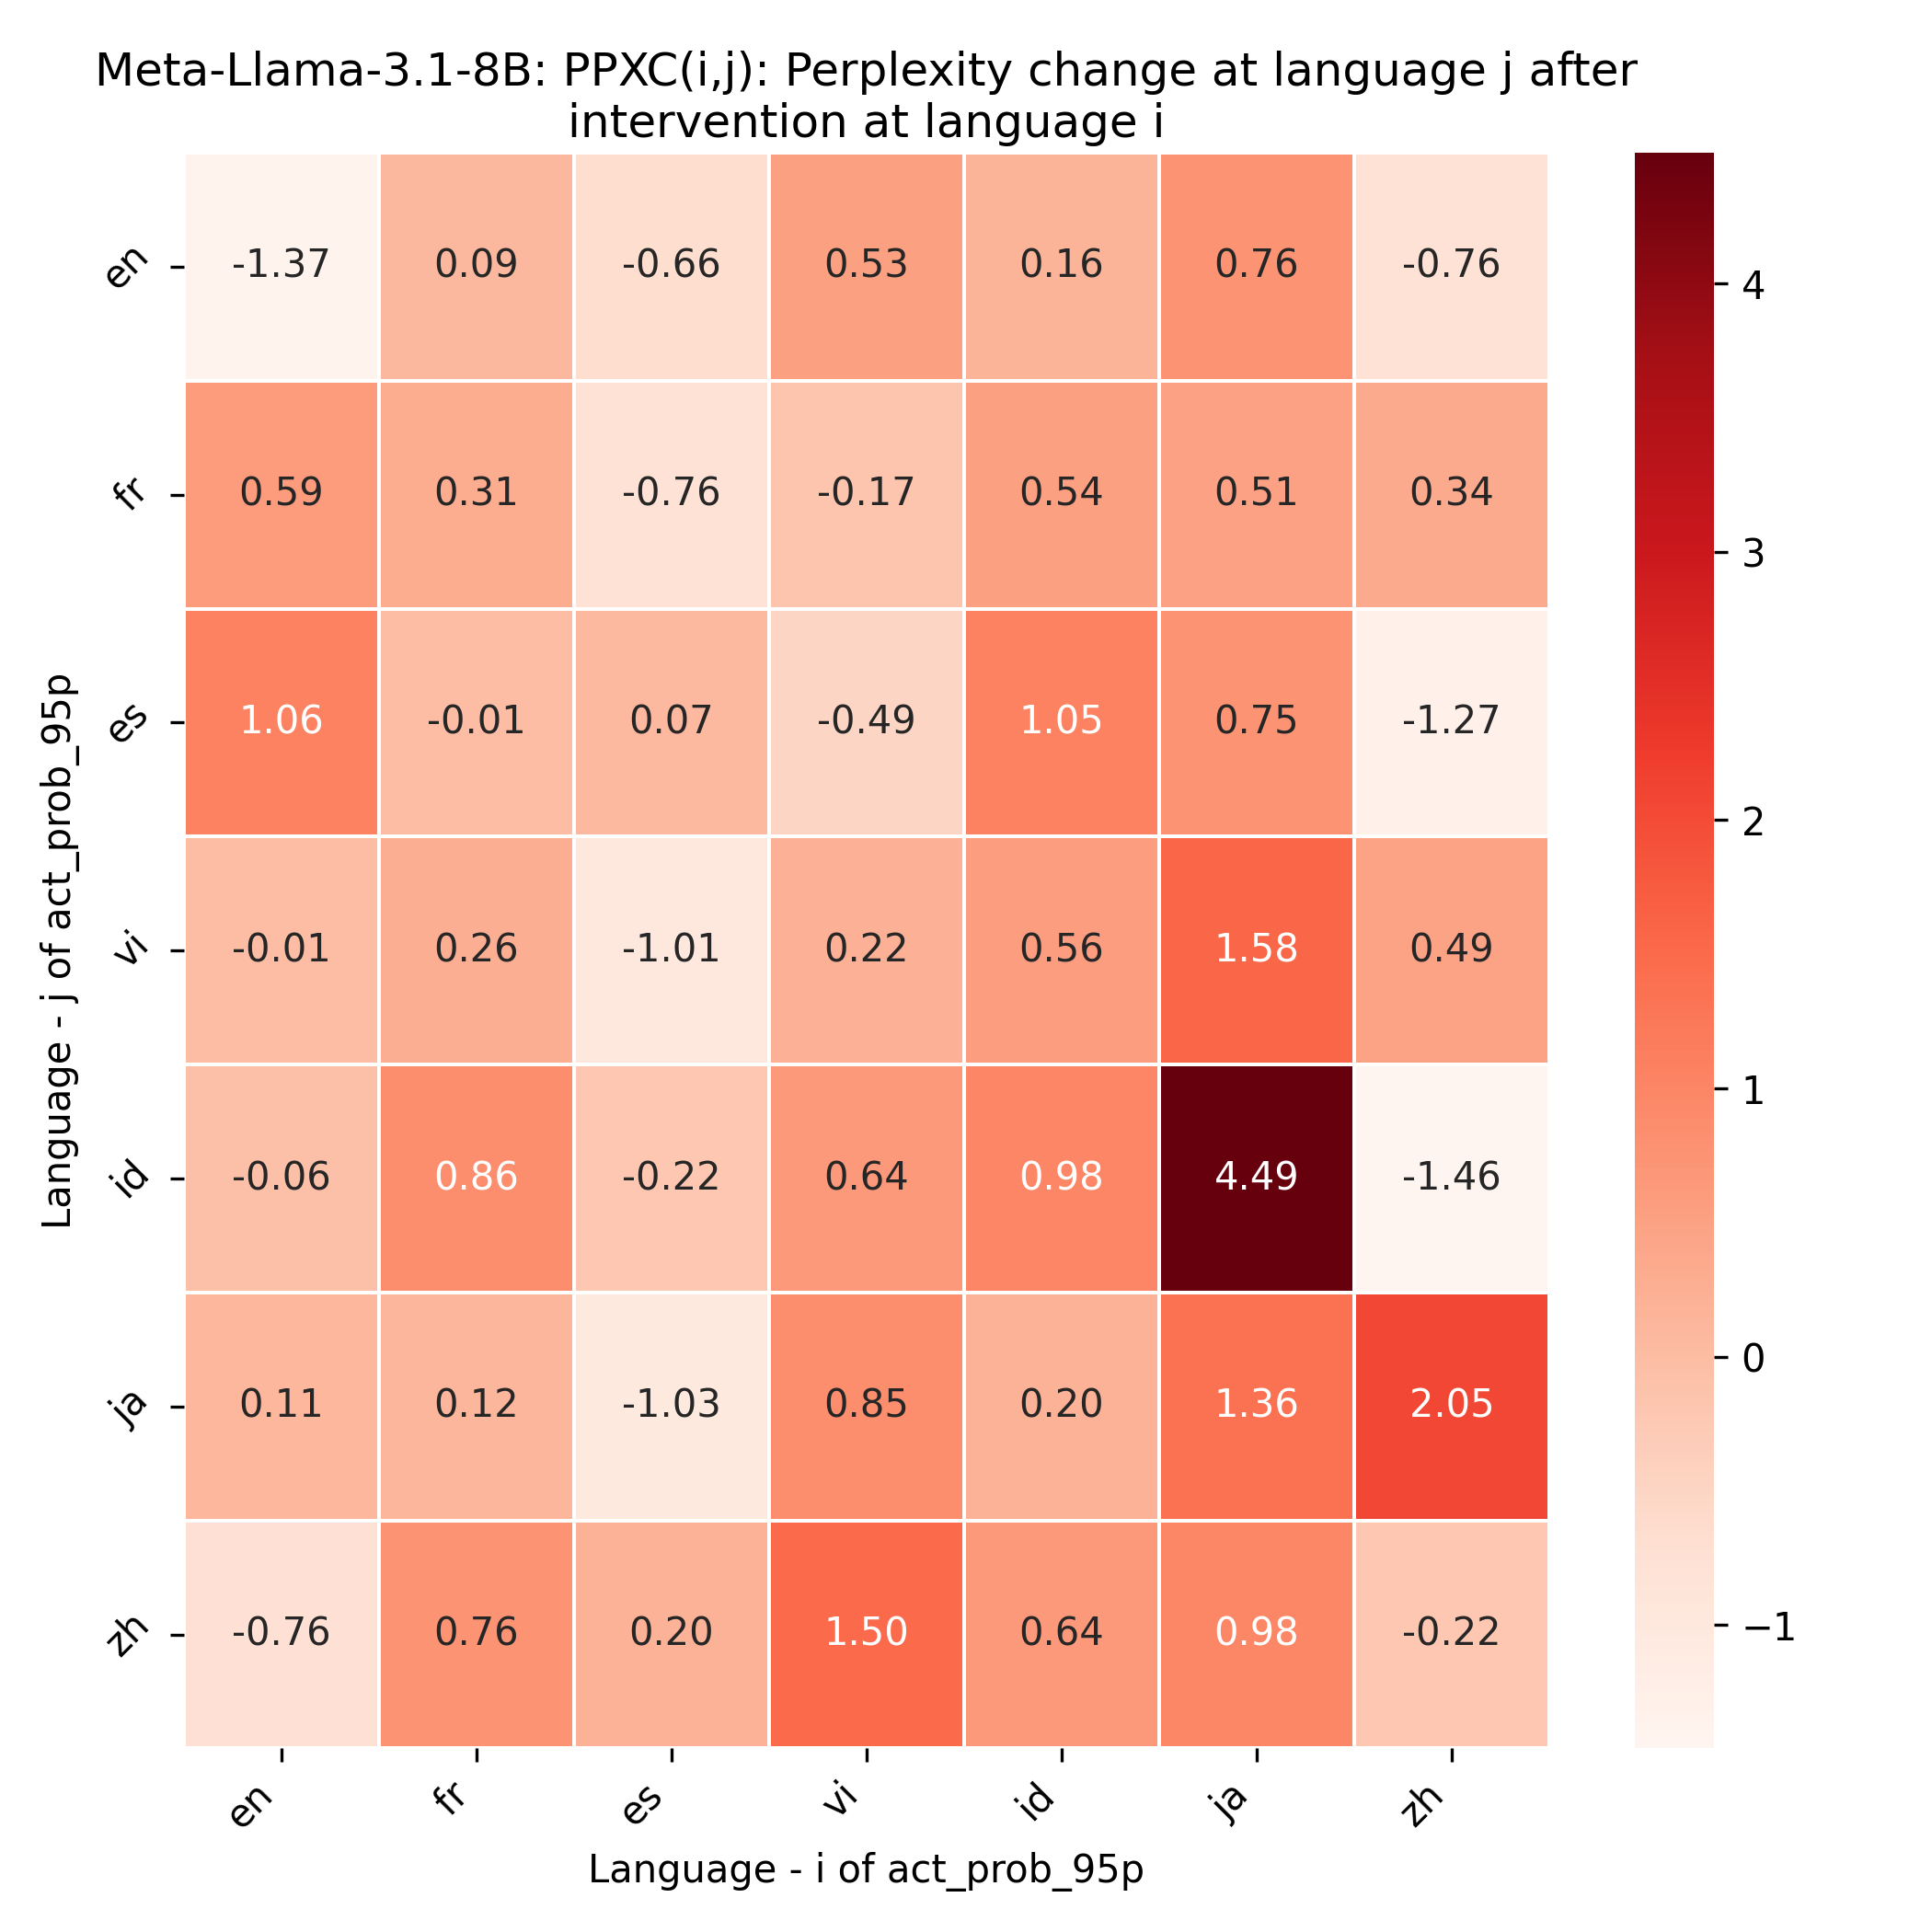
\includegraphics[width=0.45\textwidth]{Chapters/Chapter_5/perplexity/Meta-Llama-3.1-8B/act_prob_95p/ppx_change.png} \\
		\textbf{(a) PPXC for act\_prob\_zero} & \textbf{(b) PPXC for act\_prob\_90p}
	\end{tabular}
	\caption{Perplexity change $\text{PPXC}(i,j)$ for activation probability based methods.}
	\label{fig:ppxc_results}
\end{figure}

\textbf{Analysis:} From Figure \ref{fig:ppxc_results}, the following insights can be drawn:
\begin{itemize}
	\item \textbf{Non-Diagonal Behavior:} The perplexity change values are not strictly diagonal, indicating that interventions in one language (\textit{i}) can significantly influence the perplexity of another language (\textit{j}). This behavior suggests a complex interplay between the language representations within the model, where neurons may encode shared features across multiple languages.
	
	\item \textbf{Negative Values:} In some cases, the perplexity change values are negative, implying that deactivating certain neurons in one language can paradoxically improve the language capability of another. This counterintuitive result highlights the possibility that some neurons may act as bottlenecks, restricting the efficient representation of linguistic features in other languages.
	
	\item \textbf{Further Analysis Required:} The exact mechanisms underlying these phenomena are unclear and require further exploration. Factors such as the resource level of the languages, the layer-wise distribution of neurons, and the training dynamics of shared representations could play a critical role.
\end{itemize}










 
% Chapter Template

\chapter{Conclusions}\singlespacing % Main chapter title

\label{Chapter6} % Change X to a consecutive number; for referencing this chapter elsewhere, use \ref{ChapterX}

\lhead{Chapter 6. \emph{Conclusions}} % Change X to a consecutive number; this is for the header on each page - perhaps a shortened title

%----------------------------------------------------------------------------------------
%	SECTION 1
%----------------------------------------------------------------------------------------


\section{Conclusion and Future Work}

\subsection{Conclusion}
This study explored various configurations and methodologies for fine-tuning and evaluating the Meta-Llama-3.1-8B model on the XNLI task using both language-specific and task-specific neurons. The experiments leveraged LoRA (Low-Rank Adaptation) to efficiently fine-tune specific layers and subsets of neurons, ensuring minimal computational overhead while retaining robust performance. Key findings from this work include:

\begin{itemize}
	\item \textbf{Effectiveness of Statistical Interventions:} The use of statistical activation patterns, such as mean and higher quantiles (e.g., P75, P90, P95), demonstrated consistent improvements across multiple configurations. These interventions effectively optimized the performance of the model by modulating specific neurons' activation levels.
	
	\item \textbf{Language-Specific Neurons:} Results revealed that language-specific neurons computed using Wikipedia data provide strong baselines for zero-shot transfer to other languages. Fine-tuning targeted neurons, such as English-specific or Vietnamese-specific neurons, led to additional marginal improvements in performance.
	
	\item \textbf{Task-Specific Neurons:} By leveraging XNLI-specific neurons, a more task-aligned representation was achieved. The results highlighted that task-specific neurons are highly effective for fine-tuning, particularly when combined with statistical interventions on activation patterns.
	
	\item \textbf{Insights into Zero-Shot Transfer:} Unexpectedly, in some cases, the performance of zero-shot transfer models exceeded that of directly fine-tuned models. This behavior was notably observed in languages such as Urdu, suggesting the model's intrinsic robustness in certain linguistic domains.
	
	\item \textbf{Intervention with Lower Quantiles:} Activating neurons based on lower quantiles (e.g., P5, P10) provided incremental improvements, but higher quantile interventions were found to be more effective for optimizing performance across the XNLI task.
\end{itemize}

Overall, the integration of LoRA for efficient fine-tuning, combined with activation-based statistical interventions, demonstrates a promising avenue for enhancing multilingual natural language understanding. The results underline the importance of targeted neuron manipulation and its impact on language transferability and task alignment.

\subsection{Future Work}
While the results achieved in this study are promising, several avenues for future exploration remain:

\begin{itemize}
	\item \textbf{Dynamic Neuron Selection:} Future work could explore dynamic neuron selection mechanisms based on task requirements. For instance, using reinforcement learning or attention-based approaches to identify and activate neurons optimally during training and evaluation.
	
	\item \textbf{Cross-Lingual Generalization:} Investigating the impact of fine-tuning on low-resource languages and analyzing how neuron interventions affect cross-lingual generalization remains an open challenge. Additional experiments could focus on expanding the set of evaluation languages to include diverse linguistic families.
	
	\item \textbf{Integration with Larger Architectures:} Scaling the current methodologies to larger models (e.g., Meta-Llama-13B) or adapting them to more recent architectures could provide further insights into the scalability and generalization of the proposed approaches.
	
	\item \textbf{Fine-Tuning Granularity:} Exploring finer-grained levels of neuron manipulation, such as per-layer or per-head interventions, may yield better task alignment and performance across diverse benchmarks.
	
	\item \textbf{Human-Like Adaptation:} Incorporating methods inspired by human language acquisition, such as continual learning or curriculum-based fine-tuning, could enhance the model's ability to adapt to novel tasks and domains without catastrophic forgetting.
	
	\item \textbf{Interpretability and Explainability:} Further analysis is needed to understand the reasons behind certain surprising behaviors, such as why zero-shot transfer sometimes outperforms direct fine-tuning. Enhancing interpretability could shed light on the underlying mechanisms of neuron activations and their role in language understanding.
\end{itemize}

In conclusion, this study provides a strong foundation for further advancements in neuron-level fine-tuning for multilingual natural language processing. By combining efficient fine-tuning techniques with activation-based interventions, we pave the way for more adaptive and scalable language models in the future.




 
% \input{Chapters/Chapter7} 





\clearpage % Start a new page
%----------------------------------------------------------------------------------------
%	THESIS CONTENT - APPENDICES
%----------------------------------------------------------------------------------------

\addtocontents{toc}{\vspace{2em}} % Add a gap in the Contents, for aesthetics

\appendix % Cue to tell LaTeX that the following 'chapters' are Appendices

% Include the appendices of the thesis as separate files from the Appendices folder
% Uncomment the lines as you write the Appendices

% Appendix Template

\chapter{Appendix A Title} % Main appendix title

\label{AppendixA} % Change X to a consecutive letter; for referencing this appendix elsewhere, use \ref{AppendixX}

\lhead{Appendix A. \emph{Appendix A Header Title}} % Change X to a consecutive letter; this is for the header on each page - perhaps a shortened title


% Appendix Template

\chapter{Appendix B Title} % Main appendix title

\label{AppendixB} % Change X to a consecutive letter; for referencing this appendix elsewhere, use \ref{AppendixX}

\lhead{Appendix B. \emph{Appendix B Header Title}} % Change X to a consecutive letter; this is for the header on each page - perhaps a shortened title


% % Appendix Template

\chapter{APPENDIX CHAPTER TITLE} % Main appendix title

\label{AppendixC} % Change X to a consecutive letter; for referencing this appendix elsewhere, use \ref{AppendixX}

\lhead{Appendix C. \emph{APPENDIX CHAPTER TITLE}} % Change X to a consecutive letter; this is for the header on each page - perhaps a shortened title


%\input{Appendices/AppendixD}

\addtocontents{toc}{\vspace{2em}} % Add a gap in the Contents, for aesthetics

\backmatter

%----------------------------------------------------------------------------------------
%	BIBLIOGRAPHY
%----------------------------------------------------------------------------------------

\label{References}

\lhead{\emph{References}} % Change the page header to say "Bibliography"
%\usepackage{natbib}
%\renewcommand{\refname}{References}
\renewcommand\bibname{References}
\bibliographystyle{elsarticle-harv} % Use the "custom" BibTeX style for formatting the Bibliography
%\setcitestyle{authoryear,open={((},close={))}}

\bibliography{references} % The references (bibliography) information are stored in the file named "Bibliography.bib"

\newpage
% Appendix Template

\chapter{List of Publications} % Main appendix title

\label{LOP} % Change X to a consecutive letter; for referencing this appendix elsewhere, use \ref{AppendixX}

\lhead{\emph{List of Publications}} % Change X to a consecutive letter; this is for the header on each page - perhaps a shortened title

\textbf{Articles Published in International/National Journals}

\begin{enumerate}
    \item Article item 1

    \item Article item 2
\end{enumerate}

\textbf{Presentations and Proceedings in International/National Conferences}

\begin{enumerate}
    \item Conference item 1

    \item Conference item 2
\end{enumerate}
\newpage
\include{Biography}


\end{document}  
